% Options for packages loaded elsewhere
\PassOptionsToPackage{unicode}{hyperref}
\PassOptionsToPackage{hyphens}{url}
%
\documentclass[
]{article}
\usepackage{amsmath,amssymb}
\usepackage{iftex}
\ifPDFTeX
  \usepackage[T1]{fontenc}
  \usepackage[utf8]{inputenc}
  \usepackage{textcomp} % provide euro and other symbols
\else % if luatex or xetex
  \usepackage{unicode-math} % this also loads fontspec
  \defaultfontfeatures{Scale=MatchLowercase}
  \defaultfontfeatures[\rmfamily]{Ligatures=TeX,Scale=1}
\fi
\usepackage{lmodern}
\ifPDFTeX\else
  % xetex/luatex font selection
\fi
% Use upquote if available, for straight quotes in verbatim environments
\IfFileExists{upquote.sty}{\usepackage{upquote}}{}
\IfFileExists{microtype.sty}{% use microtype if available
  \usepackage[]{microtype}
  \UseMicrotypeSet[protrusion]{basicmath} % disable protrusion for tt fonts
}{}
\makeatletter
\@ifundefined{KOMAClassName}{% if non-KOMA class
  \IfFileExists{parskip.sty}{%
    \usepackage{parskip}
  }{% else
    \setlength{\parindent}{0pt}
    \setlength{\parskip}{6pt plus 2pt minus 1pt}}
}{% if KOMA class
  \KOMAoptions{parskip=half}}
\makeatother
\usepackage{xcolor}
\usepackage[margin=1in]{geometry}
\usepackage{color}
\usepackage{fancyvrb}
\newcommand{\VerbBar}{|}
\newcommand{\VERB}{\Verb[commandchars=\\\{\}]}
\DefineVerbatimEnvironment{Highlighting}{Verbatim}{commandchars=\\\{\}}
% Add ',fontsize=\small' for more characters per line
\usepackage{framed}
\definecolor{shadecolor}{RGB}{248,248,248}
\newenvironment{Shaded}{\begin{snugshade}}{\end{snugshade}}
\newcommand{\AlertTok}[1]{\textcolor[rgb]{0.94,0.16,0.16}{#1}}
\newcommand{\AnnotationTok}[1]{\textcolor[rgb]{0.56,0.35,0.01}{\textbf{\textit{#1}}}}
\newcommand{\AttributeTok}[1]{\textcolor[rgb]{0.13,0.29,0.53}{#1}}
\newcommand{\BaseNTok}[1]{\textcolor[rgb]{0.00,0.00,0.81}{#1}}
\newcommand{\BuiltInTok}[1]{#1}
\newcommand{\CharTok}[1]{\textcolor[rgb]{0.31,0.60,0.02}{#1}}
\newcommand{\CommentTok}[1]{\textcolor[rgb]{0.56,0.35,0.01}{\textit{#1}}}
\newcommand{\CommentVarTok}[1]{\textcolor[rgb]{0.56,0.35,0.01}{\textbf{\textit{#1}}}}
\newcommand{\ConstantTok}[1]{\textcolor[rgb]{0.56,0.35,0.01}{#1}}
\newcommand{\ControlFlowTok}[1]{\textcolor[rgb]{0.13,0.29,0.53}{\textbf{#1}}}
\newcommand{\DataTypeTok}[1]{\textcolor[rgb]{0.13,0.29,0.53}{#1}}
\newcommand{\DecValTok}[1]{\textcolor[rgb]{0.00,0.00,0.81}{#1}}
\newcommand{\DocumentationTok}[1]{\textcolor[rgb]{0.56,0.35,0.01}{\textbf{\textit{#1}}}}
\newcommand{\ErrorTok}[1]{\textcolor[rgb]{0.64,0.00,0.00}{\textbf{#1}}}
\newcommand{\ExtensionTok}[1]{#1}
\newcommand{\FloatTok}[1]{\textcolor[rgb]{0.00,0.00,0.81}{#1}}
\newcommand{\FunctionTok}[1]{\textcolor[rgb]{0.13,0.29,0.53}{\textbf{#1}}}
\newcommand{\ImportTok}[1]{#1}
\newcommand{\InformationTok}[1]{\textcolor[rgb]{0.56,0.35,0.01}{\textbf{\textit{#1}}}}
\newcommand{\KeywordTok}[1]{\textcolor[rgb]{0.13,0.29,0.53}{\textbf{#1}}}
\newcommand{\NormalTok}[1]{#1}
\newcommand{\OperatorTok}[1]{\textcolor[rgb]{0.81,0.36,0.00}{\textbf{#1}}}
\newcommand{\OtherTok}[1]{\textcolor[rgb]{0.56,0.35,0.01}{#1}}
\newcommand{\PreprocessorTok}[1]{\textcolor[rgb]{0.56,0.35,0.01}{\textit{#1}}}
\newcommand{\RegionMarkerTok}[1]{#1}
\newcommand{\SpecialCharTok}[1]{\textcolor[rgb]{0.81,0.36,0.00}{\textbf{#1}}}
\newcommand{\SpecialStringTok}[1]{\textcolor[rgb]{0.31,0.60,0.02}{#1}}
\newcommand{\StringTok}[1]{\textcolor[rgb]{0.31,0.60,0.02}{#1}}
\newcommand{\VariableTok}[1]{\textcolor[rgb]{0.00,0.00,0.00}{#1}}
\newcommand{\VerbatimStringTok}[1]{\textcolor[rgb]{0.31,0.60,0.02}{#1}}
\newcommand{\WarningTok}[1]{\textcolor[rgb]{0.56,0.35,0.01}{\textbf{\textit{#1}}}}
\usepackage{longtable,booktabs,array}
\usepackage{calc} % for calculating minipage widths
% Correct order of tables after \paragraph or \subparagraph
\usepackage{etoolbox}
\makeatletter
\patchcmd\longtable{\par}{\if@noskipsec\mbox{}\fi\par}{}{}
\makeatother
% Allow footnotes in longtable head/foot
\IfFileExists{footnotehyper.sty}{\usepackage{footnotehyper}}{\usepackage{footnote}}
\makesavenoteenv{longtable}
\usepackage{graphicx}
\makeatletter
\def\maxwidth{\ifdim\Gin@nat@width>\linewidth\linewidth\else\Gin@nat@width\fi}
\def\maxheight{\ifdim\Gin@nat@height>\textheight\textheight\else\Gin@nat@height\fi}
\makeatother
% Scale images if necessary, so that they will not overflow the page
% margins by default, and it is still possible to overwrite the defaults
% using explicit options in \includegraphics[width, height, ...]{}
\setkeys{Gin}{width=\maxwidth,height=\maxheight,keepaspectratio}
% Set default figure placement to htbp
\makeatletter
\def\fps@figure{htbp}
\makeatother
\setlength{\emergencystretch}{3em} % prevent overfull lines
\providecommand{\tightlist}{%
  \setlength{\itemsep}{0pt}\setlength{\parskip}{0pt}}
\setcounter{secnumdepth}{-\maxdimen} % remove section numbering
\ifLuaTeX
  \usepackage{selnolig}  % disable illegal ligatures
\fi
\usepackage{bookmark}
\IfFileExists{xurl.sty}{\usepackage{xurl}}{} % add URL line breaks if available
\urlstyle{same}
\hypersetup{
  hidelinks,
  pdfcreator={LaTeX via pandoc}}

\author{}
\date{\vspace{-2.5em}}

\begin{document}

\begin{Shaded}
\begin{Highlighting}[]
\FunctionTok{library}\NormalTok{(tidyverse)}
\end{Highlighting}
\end{Shaded}

\begin{verbatim}
## -- Attaching core tidyverse packages ------------------------ tidyverse 2.0.0 --
## v dplyr     1.1.3     v readr     2.1.4
## v forcats   1.0.0     v stringr   1.5.0
## v ggplot2   3.4.4     v tibble    3.2.1
## v lubridate 1.9.3     v tidyr     1.3.0
## v purrr     1.0.2     
## -- Conflicts ------------------------------------------ tidyverse_conflicts() --
## x dplyr::filter() masks stats::filter()
## x dplyr::lag()    masks stats::lag()
## i Use the conflicted package (<http://conflicted.r-lib.org/>) to force all conflicts to become errors
\end{verbatim}

\begin{Shaded}
\begin{Highlighting}[]
\FunctionTok{library}\NormalTok{(readxl)}
\FunctionTok{library}\NormalTok{(skimr)}
\FunctionTok{library}\NormalTok{(corrr)}
\end{Highlighting}
\end{Shaded}

\begin{verbatim}
## 
## Attache Paket: 'corrr'
## 
## Das folgende Objekt ist maskiert 'package:skimr':
## 
##     focus
\end{verbatim}

\begin{Shaded}
\begin{Highlighting}[]
\FunctionTok{library}\NormalTok{(rstanarm)}
\end{Highlighting}
\end{Shaded}

\begin{verbatim}
## Lade nötiges Paket: Rcpp
## This is rstanarm version 2.26.1
## - See https://mc-stan.org/rstanarm/articles/priors for changes to default priors!
## - Default priors may change, so it's safest to specify priors, even if equivalent to the defaults.
## - For execution on a local, multicore CPU with excess RAM we recommend calling
##   options(mc.cores = parallel::detectCores())
\end{verbatim}

\begin{Shaded}
\begin{Highlighting}[]
\FunctionTok{library}\NormalTok{(bayestestR)}
\FunctionTok{library}\NormalTok{(bayesplot)}
\end{Highlighting}
\end{Shaded}

\begin{verbatim}
## This is bayesplot version 1.10.0
## - Online documentation and vignettes at mc-stan.org/bayesplot
## - bayesplot theme set to bayesplot::theme_default()
##    * Does _not_ affect other ggplot2 plots
##    * See ?bayesplot_theme_set for details on theme setting
\end{verbatim}

\begin{Shaded}
\begin{Highlighting}[]
\FunctionTok{library}\NormalTok{(tidymodels)}
\end{Highlighting}
\end{Shaded}

\begin{verbatim}
## -- Attaching packages -------------------------------------- tidymodels 1.1.1 --
## v broom        1.0.5     v rsample      1.2.0
## v dials        1.2.0     v tune         1.1.2
## v infer        1.0.5     v workflows    1.1.3
## v modeldata    1.2.0     v workflowsets 1.0.1
## v parsnip      1.1.1     v yardstick    1.2.0
## v recipes      1.0.8     
## -- Conflicts ----------------------------------------- tidymodels_conflicts() --
## x scales::discard()   masks purrr::discard()
## x dplyr::filter()     masks stats::filter()
## x recipes::fixed()    masks stringr::fixed()
## x dplyr::lag()        masks stats::lag()
## x rsample::populate() masks Rcpp::populate()
## x yardstick::spec()   masks readr::spec()
## x recipes::step()     masks stats::step()
## * Search for functions across packages at https://www.tidymodels.org/find/
\end{verbatim}

\begin{Shaded}
\begin{Highlighting}[]
\FunctionTok{library}\NormalTok{(corrplot)}
\end{Highlighting}
\end{Shaded}

\begin{verbatim}
## corrplot 0.92 loaded
\end{verbatim}

\begin{Shaded}
\begin{Highlighting}[]
\FunctionTok{library}\NormalTok{(QuantPsyc)}
\end{Highlighting}
\end{Shaded}

\begin{verbatim}
## Warning: Paket 'QuantPsyc' wurde unter R Version 4.3.3 erstellt
\end{verbatim}

\begin{verbatim}
## Lade nötiges Paket: boot
## 
## Attache Paket: 'boot'
## 
## Das folgende Objekt ist maskiert 'package:rstanarm':
## 
##     logit
## 
## Lade nötiges Paket: MASS
## 
## Attache Paket: 'MASS'
## 
## Das folgende Objekt ist maskiert 'package:dplyr':
## 
##     select
## 
## 
## Attache Paket: 'QuantPsyc'
## 
## Das folgende Objekt ist maskiert 'package:base':
## 
##     norm
\end{verbatim}

\begin{Shaded}
\begin{Highlighting}[]
\FunctionTok{options}\NormalTok{(}\AttributeTok{mc.cores =}\NormalTok{ parallel}\SpecialCharTok{::}\FunctionTok{detectCores}\NormalTok{())}
\end{Highlighting}
\end{Shaded}

\begin{Shaded}
\begin{Highlighting}[]
\NormalTok{conflicted}\SpecialCharTok{::}\FunctionTok{conflict\_prefer}\NormalTok{(}\StringTok{"select"}\NormalTok{, }\StringTok{"dplyr"}\NormalTok{)}
\end{Highlighting}
\end{Shaded}

\begin{verbatim}
## [conflicted] Will prefer dplyr::select over any other package.
\end{verbatim}

\begin{Shaded}
\begin{Highlighting}[]
\NormalTok{conflicted}\SpecialCharTok{::}\FunctionTok{conflict\_prefer}\NormalTok{(}\StringTok{"filter"}\NormalTok{, }\StringTok{"dplyr"}\NormalTok{)}
\end{Highlighting}
\end{Shaded}

\begin{verbatim}
## [conflicted] Will prefer dplyr::filter over any other package.
\end{verbatim}

\section{1. Vorbereitung der Daten}\label{vorbereitung-der-daten}

\subsection{Daten einlesen}\label{daten-einlesen}

\begin{Shaded}
\begin{Highlighting}[]
\NormalTok{d\_raw }\OtherTok{\textless{}{-}} \FunctionTok{read\_excel}\NormalTok{(}\StringTok{"raw\_data.xlsx"}\NormalTok{)}
\end{Highlighting}
\end{Shaded}

\subsection{Unnötige Variablen
entfernen}\label{unnuxf6tige-variablen-entfernen}

\begin{Shaded}
\begin{Highlighting}[]
\NormalTok{raw1 }\OtherTok{\textless{}{-}}\NormalTok{ d\_raw }\SpecialCharTok{\%\textgreater{}\%} 
  \FunctionTok{select}\NormalTok{(}\SpecialCharTok{{-}}\FunctionTok{c}\NormalTok{(CASE, SERIAL, REF, QUESTNNR, MODE, STARTED, TIME001}\SpecialCharTok{:}\NormalTok{TIME012, MAILSENT, LASTDATA, FINISHED, Q\_VIEWER, LASTPAGE, MAXPAGE, MISSREL, MISSING))}
\end{Highlighting}
\end{Shaded}

\subsection{Variablenbeschreibung (Zeile)
entfernen}\label{variablenbeschreibung-zeile-entfernen}

\begin{Shaded}
\begin{Highlighting}[]
\NormalTok{raw1 }\OtherTok{=}\NormalTok{ raw1[}\SpecialCharTok{{-}}\DecValTok{1}\NormalTok{,]}
\end{Highlighting}
\end{Shaded}

\subsection{Spaltennamen umbenennen}\label{spaltennamen-umbenennen}

\begin{Shaded}
\begin{Highlighting}[]
\FunctionTok{names}\NormalTok{(raw1) }\OtherTok{\textless{}{-}} \FunctionTok{c}\NormalTok{(}\StringTok{"Alter"}\NormalTok{, }\StringTok{"Geschlecht"}\NormalTok{, }\StringTok{"Bildung"}\NormalTok{, }\StringTok{"Bildung\_sonstig"}\NormalTok{, }\StringTok{"BZG\_J"}\NormalTok{, }\StringTok{"BZG\_M"}\NormalTok{, }\StringTok{"Beschaeftigungsart"}\NormalTok{, }\StringTok{"Arbeitszeitmodell"}\NormalTok{, }\StringTok{"Gehalt"}\NormalTok{, }\StringTok{"Position\_im\_Unternehmen"}\NormalTok{, }\StringTok{"Remotarbeit"}\NormalTok{, }\StringTok{"IS\_K01"}\NormalTok{, }\StringTok{"IS\_K02"}\NormalTok{, }\StringTok{"IS\_K03"}\NormalTok{, }\StringTok{"IS\_K04"}\NormalTok{, }\StringTok{"IS\_E05"}\NormalTok{, }\StringTok{"IS\_E06"}\NormalTok{, }\StringTok{"IS\_E07"}\NormalTok{, }\StringTok{"IS\_E08"}\NormalTok{, }\StringTok{"OC\_A01"}\NormalTok{, }\StringTok{"OC\_A02"}\NormalTok{, }\StringTok{"OC\_A03"}\NormalTok{, }\StringTok{"OC\_A04"}\NormalTok{, }\StringTok{"OC\_A05"}\NormalTok{, }\StringTok{"CPE\_C01"}\NormalTok{, }\StringTok{"CPE\_C02"}\NormalTok{, }\StringTok{"CPE\_C03"}\NormalTok{, }\StringTok{"CPE\_C04"}\NormalTok{, }\StringTok{"CPE\_I05"}\NormalTok{, }\StringTok{"CPE\_I06"}\NormalTok{, }\StringTok{"CPE\_I07"}\NormalTok{, }\StringTok{"CPE\_I08"}\NormalTok{, }\StringTok{"CPE\_M09"}\NormalTok{, }\StringTok{"CPE\_M10"}\NormalTok{, }\StringTok{"CPE\_M11"}\NormalTok{, }\StringTok{"CPE\_M12"}\NormalTok{, }\StringTok{"CPE\_E13"}\NormalTok{, }\StringTok{"CPE\_E14"}\NormalTok{, }\StringTok{"CPE\_E15"}\NormalTok{, }\StringTok{"CPE\_E16"}\NormalTok{, }\StringTok{"PS\_01"}\NormalTok{, }\StringTok{"PS\_02"}\NormalTok{, }\StringTok{"PS\_03"}\NormalTok{, }\StringTok{"PS\_04"}\NormalTok{, }\StringTok{"PS\_05"}\NormalTok{, }\StringTok{"PS\_06"}\NormalTok{, }\StringTok{"PS\_07"}\NormalTok{, }\StringTok{"QQ\_01"}\NormalTok{, }\StringTok{"QQ\_02"}\NormalTok{, }\StringTok{"QQ\_03"}\NormalTok{, }\StringTok{"QQ\_04"}\NormalTok{, }\StringTok{"QQ\_05"}\NormalTok{, }\StringTok{"QQ\_06"}\NormalTok{, }\StringTok{"QQ\_07"}\NormalTok{, }\StringTok{"QQ\_N08"}\NormalTok{, }\StringTok{"QQ\_N09"}\NormalTok{, }\StringTok{"QQ\_N10"}\NormalTok{, }\StringTok{"QQ\_N11"}\NormalTok{, }\StringTok{"QQ\_N12"}\NormalTok{, }\StringTok{"QQ\_N13"}\NormalTok{, }\StringTok{"QQ\_N14"}\NormalTok{, }\StringTok{"SL\_01"}\NormalTok{, }\StringTok{"SL\_02"}\NormalTok{, }\StringTok{"SL\_03"}\NormalTok{, }\StringTok{"SL\_04"}\NormalTok{, }\StringTok{"SL\_05"}\NormalTok{, }\StringTok{"SL\_06"}\NormalTok{, }\StringTok{"SL\_07"}\NormalTok{, }\StringTok{"ZE01"}\NormalTok{, }\StringTok{"ZE04"}\NormalTok{, }\StringTok{"TIME\_SUM"}\NormalTok{, }\StringTok{"TIME\_RSI"}\NormalTok{)}
\end{Highlighting}
\end{Shaded}

\subsection{ID-Spalte einfügen}\label{id-spalte-einfuxfcgen}

\begin{Shaded}
\begin{Highlighting}[]
\NormalTok{raw2 }\OtherTok{\textless{}{-}}\NormalTok{ raw1 }\SpecialCharTok{\%\textgreater{}\%} 
  \FunctionTok{mutate}\NormalTok{(}\AttributeTok{ID =} \FunctionTok{row\_number}\NormalTok{()) }\SpecialCharTok{\%\textgreater{}\%} 
  \FunctionTok{select}\NormalTok{(ID, }\FunctionTok{everything}\NormalTok{())}
\end{Highlighting}
\end{Shaded}

\subsection{Kompletten Datensatz auf NA's
prüfen}\label{kompletten-datensatz-auf-nas-pruxfcfen}

\begin{Shaded}
\begin{Highlighting}[]
\FunctionTok{skim}\NormalTok{(raw2)}
\end{Highlighting}
\end{Shaded}

\begin{longtable}[]{@{}ll@{}}
\caption{Data summary}\tabularnewline
\toprule\noalign{}
\endfirsthead
\endhead
\bottomrule\noalign{}
\endlastfoot
Name & raw2 \\
Number of rows & 192 \\
Number of columns & 73 \\
\_\_\_\_\_\_\_\_\_\_\_\_\_\_\_\_\_\_\_\_\_\_\_ & \\
Column type frequency: & \\
character & 72 \\
numeric & 1 \\
\_\_\_\_\_\_\_\_\_\_\_\_\_\_\_\_\_\_\_\_\_\_\_\_ & \\
Group variables & None \\
\end{longtable}

\textbf{Variable type: character}

\begin{longtable}[]{@{}
  >{\raggedright\arraybackslash}p{(\columnwidth - 14\tabcolsep) * \real{0.2927}}
  >{\raggedleft\arraybackslash}p{(\columnwidth - 14\tabcolsep) * \real{0.1220}}
  >{\raggedleft\arraybackslash}p{(\columnwidth - 14\tabcolsep) * \real{0.1707}}
  >{\raggedleft\arraybackslash}p{(\columnwidth - 14\tabcolsep) * \real{0.0488}}
  >{\raggedleft\arraybackslash}p{(\columnwidth - 14\tabcolsep) * \real{0.0488}}
  >{\raggedleft\arraybackslash}p{(\columnwidth - 14\tabcolsep) * \real{0.0732}}
  >{\raggedleft\arraybackslash}p{(\columnwidth - 14\tabcolsep) * \real{0.1098}}
  >{\raggedleft\arraybackslash}p{(\columnwidth - 14\tabcolsep) * \real{0.1341}}@{}}
\toprule\noalign{}
\begin{minipage}[b]{\linewidth}\raggedright
skim\_variable
\end{minipage} & \begin{minipage}[b]{\linewidth}\raggedleft
n\_missing
\end{minipage} & \begin{minipage}[b]{\linewidth}\raggedleft
complete\_rate
\end{minipage} & \begin{minipage}[b]{\linewidth}\raggedleft
min
\end{minipage} & \begin{minipage}[b]{\linewidth}\raggedleft
max
\end{minipage} & \begin{minipage}[b]{\linewidth}\raggedleft
empty
\end{minipage} & \begin{minipage}[b]{\linewidth}\raggedleft
n\_unique
\end{minipage} & \begin{minipage}[b]{\linewidth}\raggedleft
whitespace
\end{minipage} \\
\midrule\noalign{}
\endhead
\bottomrule\noalign{}
\endlastfoot
Alter & 2 & 0.99 & 2 & 2 & 0 & 39 & 0 \\
Geschlecht & 0 & 1.00 & 1 & 1 & 0 & 2 & 0 \\
Bildung & 0 & 1.00 & 1 & 1 & 0 & 8 & 0 \\
Bildung\_sonstig & 189 & 0.02 & 12 & 17 & 0 & 3 & 0 \\
BZG\_J & 0 & 1.00 & 1 & 2 & 0 & 38 & 0 \\
BZG\_M & 5 & 0.97 & 1 & 2 & 0 & 12 & 0 \\
Beschaeftigungsart & 0 & 1.00 & 1 & 1 & 0 & 2 & 0 \\
Arbeitszeitmodell & 0 & 1.00 & 1 & 5 & 0 & 40 & 0 \\
Gehalt & 2 & 0.99 & 1 & 1 & 0 & 7 & 0 \\
Position\_im\_Unternehmen & 0 & 1.00 & 1 & 1 & 0 & 4 & 0 \\
Remotarbeit & 0 & 1.00 & 1 & 1 & 0 & 6 & 0 \\
IS\_K01 & 0 & 1.00 & 1 & 1 & 0 & 7 & 0 \\
IS\_K02 & 0 & 1.00 & 1 & 1 & 0 & 7 & 0 \\
IS\_K03 & 0 & 1.00 & 1 & 1 & 0 & 7 & 0 \\
IS\_K04 & 0 & 1.00 & 1 & 1 & 0 & 7 & 0 \\
IS\_E05 & 0 & 1.00 & 1 & 1 & 0 & 7 & 0 \\
IS\_E06 & 0 & 1.00 & 1 & 1 & 0 & 7 & 0 \\
IS\_E07 & 0 & 1.00 & 1 & 1 & 0 & 7 & 0 \\
IS\_E08 & 0 & 1.00 & 1 & 1 & 0 & 7 & 0 \\
OC\_A01 & 0 & 1.00 & 1 & 1 & 0 & 5 & 0 \\
OC\_A02 & 0 & 1.00 & 1 & 1 & 0 & 5 & 0 \\
OC\_A03 & 0 & 1.00 & 1 & 1 & 0 & 5 & 0 \\
OC\_A04 & 0 & 1.00 & 1 & 1 & 0 & 5 & 0 \\
OC\_A05 & 0 & 1.00 & 1 & 1 & 0 & 5 & 0 \\
CPE\_C01 & 0 & 1.00 & 1 & 1 & 0 & 7 & 0 \\
CPE\_C02 & 0 & 1.00 & 1 & 1 & 0 & 7 & 0 \\
CPE\_C03 & 0 & 1.00 & 1 & 1 & 0 & 7 & 0 \\
CPE\_C04 & 0 & 1.00 & 1 & 1 & 0 & 7 & 0 \\
CPE\_I05 & 0 & 1.00 & 1 & 1 & 0 & 7 & 0 \\
CPE\_I06 & 0 & 1.00 & 1 & 1 & 0 & 7 & 0 \\
CPE\_I07 & 0 & 1.00 & 1 & 1 & 0 & 7 & 0 \\
CPE\_I08 & 0 & 1.00 & 1 & 1 & 0 & 7 & 0 \\
CPE\_M09 & 0 & 1.00 & 1 & 1 & 0 & 7 & 0 \\
CPE\_M10 & 0 & 1.00 & 1 & 1 & 0 & 7 & 0 \\
CPE\_M11 & 1 & 0.99 & 1 & 1 & 0 & 7 & 0 \\
CPE\_M12 & 0 & 1.00 & 1 & 1 & 0 & 7 & 0 \\
CPE\_E13 & 0 & 1.00 & 1 & 1 & 0 & 7 & 0 \\
CPE\_E14 & 0 & 1.00 & 1 & 1 & 0 & 7 & 0 \\
CPE\_E15 & 0 & 1.00 & 1 & 1 & 0 & 7 & 0 \\
CPE\_E16 & 0 & 1.00 & 1 & 1 & 0 & 7 & 0 \\
PS\_01 & 0 & 1.00 & 1 & 1 & 0 & 7 & 0 \\
PS\_02 & 0 & 1.00 & 1 & 1 & 0 & 7 & 0 \\
PS\_03 & 0 & 1.00 & 1 & 1 & 0 & 7 & 0 \\
PS\_04 & 0 & 1.00 & 1 & 1 & 0 & 7 & 0 \\
PS\_05 & 0 & 1.00 & 1 & 1 & 0 & 7 & 0 \\
PS\_06 & 0 & 1.00 & 1 & 1 & 0 & 7 & 0 \\
PS\_07 & 0 & 1.00 & 1 & 1 & 0 & 7 & 0 \\
QQ\_01 & 0 & 1.00 & 1 & 1 & 0 & 5 & 0 \\
QQ\_02 & 0 & 1.00 & 1 & 1 & 0 & 5 & 0 \\
QQ\_03 & 0 & 1.00 & 1 & 1 & 0 & 5 & 0 \\
QQ\_04 & 0 & 1.00 & 1 & 1 & 0 & 5 & 0 \\
QQ\_05 & 0 & 1.00 & 1 & 1 & 0 & 5 & 0 \\
QQ\_06 & 0 & 1.00 & 1 & 1 & 0 & 5 & 0 \\
QQ\_07 & 0 & 1.00 & 1 & 1 & 0 & 5 & 0 \\
QQ\_N08 & 0 & 1.00 & 1 & 1 & 0 & 5 & 0 \\
QQ\_N09 & 0 & 1.00 & 1 & 1 & 0 & 5 & 0 \\
QQ\_N10 & 0 & 1.00 & 1 & 1 & 0 & 5 & 0 \\
QQ\_N11 & 0 & 1.00 & 1 & 1 & 0 & 5 & 0 \\
QQ\_N12 & 0 & 1.00 & 1 & 1 & 0 & 5 & 0 \\
QQ\_N13 & 0 & 1.00 & 1 & 1 & 0 & 5 & 0 \\
QQ\_N14 & 0 & 1.00 & 1 & 1 & 0 & 5 & 0 \\
SL\_01 & 0 & 1.00 & 1 & 1 & 0 & 7 & 0 \\
SL\_02 & 0 & 1.00 & 1 & 1 & 0 & 7 & 0 \\
SL\_03 & 0 & 1.00 & 1 & 1 & 0 & 7 & 0 \\
SL\_04 & 0 & 1.00 & 1 & 1 & 0 & 7 & 0 \\
SL\_05 & 1 & 0.99 & 1 & 1 & 0 & 7 & 0 \\
SL\_06 & 0 & 1.00 & 1 & 1 & 0 & 7 & 0 \\
SL\_07 & 0 & 1.00 & 1 & 1 & 0 & 7 & 0 \\
ZE01 & 0 & 1.00 & 1 & 1 & 0 & 1 & 0 \\
ZE04 & 0 & 1.00 & 1 & 1 & 0 & 1 & 0 \\
TIME\_SUM & 0 & 1.00 & 3 & 4 & 0 & 167 & 0 \\
TIME\_RSI & 0 & 1.00 & 1 & 4 & 0 & 111 & 0 \\
\end{longtable}

\textbf{Variable type: numeric}

\begin{longtable}[]{@{}
  >{\raggedright\arraybackslash}p{(\columnwidth - 20\tabcolsep) * \real{0.1728}}
  >{\raggedleft\arraybackslash}p{(\columnwidth - 20\tabcolsep) * \real{0.1235}}
  >{\raggedleft\arraybackslash}p{(\columnwidth - 20\tabcolsep) * \real{0.1728}}
  >{\raggedleft\arraybackslash}p{(\columnwidth - 20\tabcolsep) * \real{0.0617}}
  >{\raggedleft\arraybackslash}p{(\columnwidth - 20\tabcolsep) * \real{0.0741}}
  >{\raggedleft\arraybackslash}p{(\columnwidth - 20\tabcolsep) * \real{0.0370}}
  >{\raggedleft\arraybackslash}p{(\columnwidth - 20\tabcolsep) * \real{0.0741}}
  >{\raggedleft\arraybackslash}p{(\columnwidth - 20\tabcolsep) * \real{0.0617}}
  >{\raggedleft\arraybackslash}p{(\columnwidth - 20\tabcolsep) * \real{0.0864}}
  >{\raggedleft\arraybackslash}p{(\columnwidth - 20\tabcolsep) * \real{0.0617}}
  >{\raggedright\arraybackslash}p{(\columnwidth - 20\tabcolsep) * \real{0.0741}}@{}}
\toprule\noalign{}
\begin{minipage}[b]{\linewidth}\raggedright
skim\_variable
\end{minipage} & \begin{minipage}[b]{\linewidth}\raggedleft
n\_missing
\end{minipage} & \begin{minipage}[b]{\linewidth}\raggedleft
complete\_rate
\end{minipage} & \begin{minipage}[b]{\linewidth}\raggedleft
mean
\end{minipage} & \begin{minipage}[b]{\linewidth}\raggedleft
sd
\end{minipage} & \begin{minipage}[b]{\linewidth}\raggedleft
p0
\end{minipage} & \begin{minipage}[b]{\linewidth}\raggedleft
p25
\end{minipage} & \begin{minipage}[b]{\linewidth}\raggedleft
p50
\end{minipage} & \begin{minipage}[b]{\linewidth}\raggedleft
p75
\end{minipage} & \begin{minipage}[b]{\linewidth}\raggedleft
p100
\end{minipage} & \begin{minipage}[b]{\linewidth}\raggedright
hist
\end{minipage} \\
\midrule\noalign{}
\endhead
\bottomrule\noalign{}
\endlastfoot
ID & 0 & 1 & 96.5 & 55.57 & 1 & 48.75 & 96.5 & 144.25 & 192 & ▇▇▇▇▇ \\
\end{longtable}

\begin{quote}
NA bei CPE\_M11 \& SL\_05 --\textgreater{} wird als NA mit in die
Zeilenmittelwerte mit einberechnet!
\end{quote}

\section{2. Negative gepolte Items
prüfen}\label{negative-gepolte-items-pruxfcfen}

\subsection{Recodieren der Psychologische Sicherheit
Items}\label{recodieren-der-psychologische-sicherheit-items}

\begin{Shaded}
\begin{Highlighting}[]
\NormalTok{raw3 }\OtherTok{\textless{}{-}}\NormalTok{ raw2 }\SpecialCharTok{\%\textgreater{}\%} 
  \FunctionTok{mutate}\NormalTok{(}\FunctionTok{across}\NormalTok{(}
    \AttributeTok{.cols =} \FunctionTok{c}\NormalTok{(PS\_03, PS\_05, PS\_06),}
    \AttributeTok{.fns =} \SpecialCharTok{\textasciitilde{}}\NormalTok{ dplyr}\SpecialCharTok{::}\FunctionTok{recode}\NormalTok{(.,}
                    \StringTok{\textasciigrave{}}\AttributeTok{1}\StringTok{\textasciigrave{}} \OtherTok{=} \DecValTok{7}\NormalTok{,}
                    \StringTok{\textasciigrave{}}\AttributeTok{2}\StringTok{\textasciigrave{}} \OtherTok{=} \DecValTok{6}\NormalTok{,}
                    \StringTok{\textasciigrave{}}\AttributeTok{3}\StringTok{\textasciigrave{}} \OtherTok{=} \DecValTok{5}\NormalTok{,}
                    \StringTok{\textasciigrave{}}\AttributeTok{4}\StringTok{\textasciigrave{}} \OtherTok{=} \DecValTok{4}\NormalTok{,}
                    \StringTok{\textasciigrave{}}\AttributeTok{5}\StringTok{\textasciigrave{}} \OtherTok{=} \DecValTok{3}\NormalTok{,}
                    \StringTok{\textasciigrave{}}\AttributeTok{6}\StringTok{\textasciigrave{}} \OtherTok{=} \DecValTok{2}\NormalTok{,}
                    \StringTok{\textasciigrave{}}\AttributeTok{7}\StringTok{\textasciigrave{}} \OtherTok{=} \DecValTok{1}\NormalTok{)))}
\end{Highlighting}
\end{Shaded}

\subsection{Recodieren des organisationalen
Commitments}\label{recodieren-des-organisationalen-commitments}

\begin{Shaded}
\begin{Highlighting}[]
\NormalTok{raw4 }\OtherTok{\textless{}{-}}\NormalTok{ raw3 }\SpecialCharTok{\%\textgreater{}\%} 
  \FunctionTok{mutate}\NormalTok{(}\FunctionTok{across}\NormalTok{(}
    \AttributeTok{.cols =}\NormalTok{ OC\_A02,}
    \AttributeTok{.fns =} \SpecialCharTok{\textasciitilde{}}\NormalTok{dplyr}\SpecialCharTok{::}\FunctionTok{recode}\NormalTok{(.,}
                    \StringTok{\textasciigrave{}}\AttributeTok{1}\StringTok{\textasciigrave{}} \OtherTok{=} \DecValTok{5}\NormalTok{,}
                    \StringTok{\textasciigrave{}}\AttributeTok{2}\StringTok{\textasciigrave{}} \OtherTok{=} \DecValTok{4}\NormalTok{,}
                    \StringTok{\textasciigrave{}}\AttributeTok{3}\StringTok{\textasciigrave{}} \OtherTok{=} \DecValTok{3}\NormalTok{,}
                    \StringTok{\textasciigrave{}}\AttributeTok{4}\StringTok{\textasciigrave{}} \OtherTok{=} \DecValTok{2}\NormalTok{,}
                    \StringTok{\textasciigrave{}}\AttributeTok{5}\StringTok{\textasciigrave{}} \OtherTok{=} \DecValTok{1}\NormalTok{)))}
\end{Highlighting}
\end{Shaded}

\section{3. Variablen umkodieren}\label{variablen-umkodieren}

\begin{Shaded}
\begin{Highlighting}[]
\NormalTok{raw4}\SpecialCharTok{$}\NormalTok{Geschlecht }\OtherTok{\textless{}{-}} \FunctionTok{as.numeric}\NormalTok{(raw4}\SpecialCharTok{$}\NormalTok{Geschlecht)}
\NormalTok{raw4}\SpecialCharTok{$}\NormalTok{Alter }\OtherTok{\textless{}{-}} \FunctionTok{as.numeric}\NormalTok{(raw4}\SpecialCharTok{$}\NormalTok{Alter)}
\NormalTok{raw4}\SpecialCharTok{$}\NormalTok{Bildung }\OtherTok{\textless{}{-}} \FunctionTok{as.numeric}\NormalTok{(raw4}\SpecialCharTok{$}\NormalTok{Bildung)}
\NormalTok{raw4}\SpecialCharTok{$}\NormalTok{BZG\_J }\OtherTok{\textless{}{-}} \FunctionTok{as.numeric}\NormalTok{(raw4}\SpecialCharTok{$}\NormalTok{BZG\_J)}
\NormalTok{raw4}\SpecialCharTok{$}\NormalTok{BZG\_M }\OtherTok{\textless{}{-}} \FunctionTok{as.numeric}\NormalTok{(raw4}\SpecialCharTok{$}\NormalTok{BZG\_M)}
\NormalTok{raw4}\SpecialCharTok{$}\NormalTok{Arbeitszeitmodell }\OtherTok{\textless{}{-}} \FunctionTok{as.numeric}\NormalTok{(raw4}\SpecialCharTok{$}\NormalTok{Arbeitszeitmodell)}
\NormalTok{raw4}\SpecialCharTok{$}\NormalTok{Beschaeftigungsart }\OtherTok{\textless{}{-}} \FunctionTok{as.numeric}\NormalTok{(raw4}\SpecialCharTok{$}\NormalTok{Beschaeftigungsart)}
\NormalTok{raw4}\SpecialCharTok{$}\NormalTok{Gehalt }\OtherTok{\textless{}{-}} \FunctionTok{as.numeric}\NormalTok{(raw4}\SpecialCharTok{$}\NormalTok{Gehalt)}
\NormalTok{raw4}\SpecialCharTok{$}\NormalTok{Position\_im\_Unternehmen }\OtherTok{\textless{}{-}} \FunctionTok{as.numeric}\NormalTok{(raw4}\SpecialCharTok{$}\NormalTok{Position\_im\_Unternehmen)}
\NormalTok{raw4}\SpecialCharTok{$}\NormalTok{Remotarbeit }\OtherTok{\textless{}{-}} \FunctionTok{as.numeric}\NormalTok{(raw4}\SpecialCharTok{$}\NormalTok{Remotarbeit)}
\end{Highlighting}
\end{Shaded}

\begin{Shaded}
\begin{Highlighting}[]
\NormalTok{raw4}\SpecialCharTok{$}\NormalTok{IS\_K01 }\OtherTok{\textless{}{-}} \FunctionTok{as.numeric}\NormalTok{(raw4}\SpecialCharTok{$}\NormalTok{IS\_K01)}
\NormalTok{raw4}\SpecialCharTok{$}\NormalTok{IS\_K02 }\OtherTok{\textless{}{-}} \FunctionTok{as.numeric}\NormalTok{(raw4}\SpecialCharTok{$}\NormalTok{IS\_K02)}
\NormalTok{raw4}\SpecialCharTok{$}\NormalTok{IS\_K03 }\OtherTok{\textless{}{-}} \FunctionTok{as.numeric}\NormalTok{(raw4}\SpecialCharTok{$}\NormalTok{IS\_K03)}
\NormalTok{raw4}\SpecialCharTok{$}\NormalTok{IS\_K04 }\OtherTok{\textless{}{-}} \FunctionTok{as.numeric}\NormalTok{(raw4}\SpecialCharTok{$}\NormalTok{IS\_K04)}
\NormalTok{raw4}\SpecialCharTok{$}\NormalTok{IS\_E05 }\OtherTok{\textless{}{-}} \FunctionTok{as.numeric}\NormalTok{(raw4}\SpecialCharTok{$}\NormalTok{IS\_E05)}
\NormalTok{raw4}\SpecialCharTok{$}\NormalTok{IS\_E06 }\OtherTok{\textless{}{-}} \FunctionTok{as.numeric}\NormalTok{(raw4}\SpecialCharTok{$}\NormalTok{IS\_E06)}
\NormalTok{raw4}\SpecialCharTok{$}\NormalTok{IS\_E07 }\OtherTok{\textless{}{-}} \FunctionTok{as.numeric}\NormalTok{(raw4}\SpecialCharTok{$}\NormalTok{IS\_E07)}
\NormalTok{raw4}\SpecialCharTok{$}\NormalTok{IS\_E08 }\OtherTok{\textless{}{-}} \FunctionTok{as.numeric}\NormalTok{(raw4}\SpecialCharTok{$}\NormalTok{IS\_E08)}
\end{Highlighting}
\end{Shaded}

\begin{Shaded}
\begin{Highlighting}[]
\NormalTok{raw4}\SpecialCharTok{$}\NormalTok{OC\_A01 }\OtherTok{\textless{}{-}} \FunctionTok{as.numeric}\NormalTok{(raw4}\SpecialCharTok{$}\NormalTok{OC\_A01)}
\NormalTok{raw4}\SpecialCharTok{$}\NormalTok{OC\_A02 }\OtherTok{\textless{}{-}} \FunctionTok{as.numeric}\NormalTok{(raw4}\SpecialCharTok{$}\NormalTok{OC\_A02)}
\NormalTok{raw4}\SpecialCharTok{$}\NormalTok{OC\_A03 }\OtherTok{\textless{}{-}} \FunctionTok{as.numeric}\NormalTok{(raw4}\SpecialCharTok{$}\NormalTok{OC\_A03)}
\NormalTok{raw4}\SpecialCharTok{$}\NormalTok{OC\_A04 }\OtherTok{\textless{}{-}} \FunctionTok{as.numeric}\NormalTok{(raw4}\SpecialCharTok{$}\NormalTok{OC\_A04)}
\NormalTok{raw4}\SpecialCharTok{$}\NormalTok{OC\_A05 }\OtherTok{\textless{}{-}} \FunctionTok{as.numeric}\NormalTok{(raw4}\SpecialCharTok{$}\NormalTok{OC\_A05)}
\end{Highlighting}
\end{Shaded}

\begin{Shaded}
\begin{Highlighting}[]
\NormalTok{raw4}\SpecialCharTok{$}\NormalTok{CPE\_C01 }\OtherTok{\textless{}{-}} \FunctionTok{as.numeric}\NormalTok{(raw4}\SpecialCharTok{$}\NormalTok{CPE\_C01)}
\NormalTok{raw4}\SpecialCharTok{$}\NormalTok{CPE\_C02 }\OtherTok{\textless{}{-}} \FunctionTok{as.numeric}\NormalTok{(raw4}\SpecialCharTok{$}\NormalTok{CPE\_C02)}
\NormalTok{raw4}\SpecialCharTok{$}\NormalTok{CPE\_C03 }\OtherTok{\textless{}{-}} \FunctionTok{as.numeric}\NormalTok{(raw4}\SpecialCharTok{$}\NormalTok{CPE\_C03)}
\NormalTok{raw4}\SpecialCharTok{$}\NormalTok{CPE\_C04 }\OtherTok{\textless{}{-}} \FunctionTok{as.numeric}\NormalTok{(raw4}\SpecialCharTok{$}\NormalTok{CPE\_C04)}
\NormalTok{raw4}\SpecialCharTok{$}\NormalTok{CPE\_I05 }\OtherTok{\textless{}{-}} \FunctionTok{as.numeric}\NormalTok{(raw4}\SpecialCharTok{$}\NormalTok{CPE\_I05)}
\NormalTok{raw4}\SpecialCharTok{$}\NormalTok{CPE\_I06 }\OtherTok{\textless{}{-}} \FunctionTok{as.numeric}\NormalTok{(raw4}\SpecialCharTok{$}\NormalTok{CPE\_I06)}
\NormalTok{raw4}\SpecialCharTok{$}\NormalTok{CPE\_I07 }\OtherTok{\textless{}{-}} \FunctionTok{as.numeric}\NormalTok{(raw4}\SpecialCharTok{$}\NormalTok{CPE\_I07)}
\NormalTok{raw4}\SpecialCharTok{$}\NormalTok{CPE\_I08 }\OtherTok{\textless{}{-}} \FunctionTok{as.numeric}\NormalTok{(raw4}\SpecialCharTok{$}\NormalTok{CPE\_I08)}
\NormalTok{raw4}\SpecialCharTok{$}\NormalTok{CPE\_M09 }\OtherTok{\textless{}{-}} \FunctionTok{as.numeric}\NormalTok{(raw4}\SpecialCharTok{$}\NormalTok{CPE\_M09)}
\NormalTok{raw4}\SpecialCharTok{$}\NormalTok{CPE\_M10 }\OtherTok{\textless{}{-}} \FunctionTok{as.numeric}\NormalTok{(raw4}\SpecialCharTok{$}\NormalTok{CPE\_M10)}
\NormalTok{raw4}\SpecialCharTok{$}\NormalTok{CPE\_M11 }\OtherTok{\textless{}{-}} \FunctionTok{as.numeric}\NormalTok{(raw4}\SpecialCharTok{$}\NormalTok{CPE\_M11)}
\NormalTok{raw4}\SpecialCharTok{$}\NormalTok{CPE\_M12 }\OtherTok{\textless{}{-}} \FunctionTok{as.numeric}\NormalTok{(raw4}\SpecialCharTok{$}\NormalTok{CPE\_M12)}
\NormalTok{raw4}\SpecialCharTok{$}\NormalTok{CPE\_E13 }\OtherTok{\textless{}{-}} \FunctionTok{as.numeric}\NormalTok{(raw4}\SpecialCharTok{$}\NormalTok{CPE\_E13)}
\NormalTok{raw4}\SpecialCharTok{$}\NormalTok{CPE\_E14 }\OtherTok{\textless{}{-}} \FunctionTok{as.numeric}\NormalTok{(raw4}\SpecialCharTok{$}\NormalTok{CPE\_E14)}
\NormalTok{raw4}\SpecialCharTok{$}\NormalTok{CPE\_E15 }\OtherTok{\textless{}{-}} \FunctionTok{as.numeric}\NormalTok{(raw4}\SpecialCharTok{$}\NormalTok{CPE\_E15)}
\NormalTok{raw4}\SpecialCharTok{$}\NormalTok{CPE\_E16 }\OtherTok{\textless{}{-}} \FunctionTok{as.numeric}\NormalTok{(raw4}\SpecialCharTok{$}\NormalTok{CPE\_E16)}
\end{Highlighting}
\end{Shaded}

\begin{Shaded}
\begin{Highlighting}[]
\NormalTok{raw4}\SpecialCharTok{$}\NormalTok{PS\_01 }\OtherTok{\textless{}{-}} \FunctionTok{as.numeric}\NormalTok{(raw4}\SpecialCharTok{$}\NormalTok{PS\_01)}
\NormalTok{raw4}\SpecialCharTok{$}\NormalTok{PS\_02 }\OtherTok{\textless{}{-}} \FunctionTok{as.numeric}\NormalTok{(raw4}\SpecialCharTok{$}\NormalTok{PS\_02)}
\NormalTok{raw4}\SpecialCharTok{$}\NormalTok{PS\_03 }\OtherTok{\textless{}{-}} \FunctionTok{as.numeric}\NormalTok{(raw4}\SpecialCharTok{$}\NormalTok{PS\_03)}
\NormalTok{raw4}\SpecialCharTok{$}\NormalTok{PS\_04 }\OtherTok{\textless{}{-}} \FunctionTok{as.numeric}\NormalTok{(raw4}\SpecialCharTok{$}\NormalTok{PS\_04)}
\NormalTok{raw4}\SpecialCharTok{$}\NormalTok{PS\_05 }\OtherTok{\textless{}{-}} \FunctionTok{as.numeric}\NormalTok{(raw4}\SpecialCharTok{$}\NormalTok{PS\_05)}
\NormalTok{raw4}\SpecialCharTok{$}\NormalTok{PS\_06 }\OtherTok{\textless{}{-}} \FunctionTok{as.numeric}\NormalTok{(raw4}\SpecialCharTok{$}\NormalTok{PS\_06)}
\NormalTok{raw4}\SpecialCharTok{$}\NormalTok{PS\_07 }\OtherTok{\textless{}{-}} \FunctionTok{as.numeric}\NormalTok{(raw4}\SpecialCharTok{$}\NormalTok{PS\_07)}
\end{Highlighting}
\end{Shaded}

\begin{Shaded}
\begin{Highlighting}[]
\NormalTok{raw4}\SpecialCharTok{$}\NormalTok{QQ\_01 }\OtherTok{\textless{}{-}} \FunctionTok{as.numeric}\NormalTok{(raw4}\SpecialCharTok{$}\NormalTok{QQ\_01)}
\NormalTok{raw4}\SpecialCharTok{$}\NormalTok{QQ\_02 }\OtherTok{\textless{}{-}} \FunctionTok{as.numeric}\NormalTok{(raw4}\SpecialCharTok{$}\NormalTok{QQ\_02)}
\NormalTok{raw4}\SpecialCharTok{$}\NormalTok{QQ\_03 }\OtherTok{\textless{}{-}} \FunctionTok{as.numeric}\NormalTok{(raw4}\SpecialCharTok{$}\NormalTok{QQ\_03)}
\NormalTok{raw4}\SpecialCharTok{$}\NormalTok{QQ\_04 }\OtherTok{\textless{}{-}} \FunctionTok{as.numeric}\NormalTok{(raw4}\SpecialCharTok{$}\NormalTok{QQ\_04)}
\NormalTok{raw4}\SpecialCharTok{$}\NormalTok{QQ\_05 }\OtherTok{\textless{}{-}} \FunctionTok{as.numeric}\NormalTok{(raw4}\SpecialCharTok{$}\NormalTok{QQ\_05)}
\NormalTok{raw4}\SpecialCharTok{$}\NormalTok{QQ\_06 }\OtherTok{\textless{}{-}} \FunctionTok{as.numeric}\NormalTok{(raw4}\SpecialCharTok{$}\NormalTok{QQ\_06)}
\NormalTok{raw4}\SpecialCharTok{$}\NormalTok{QQ\_07 }\OtherTok{\textless{}{-}} \FunctionTok{as.numeric}\NormalTok{(raw4}\SpecialCharTok{$}\NormalTok{QQ\_07)}
\end{Highlighting}
\end{Shaded}

\begin{Shaded}
\begin{Highlighting}[]
\NormalTok{raw4}\SpecialCharTok{$}\NormalTok{QQ\_N08 }\OtherTok{\textless{}{-}} \FunctionTok{as.numeric}\NormalTok{(raw4}\SpecialCharTok{$}\NormalTok{QQ\_N08)}
\NormalTok{raw4}\SpecialCharTok{$}\NormalTok{QQ\_N09 }\OtherTok{\textless{}{-}} \FunctionTok{as.numeric}\NormalTok{(raw4}\SpecialCharTok{$}\NormalTok{QQ\_N09)}
\NormalTok{raw4}\SpecialCharTok{$}\NormalTok{QQ\_N10 }\OtherTok{\textless{}{-}} \FunctionTok{as.numeric}\NormalTok{(raw4}\SpecialCharTok{$}\NormalTok{QQ\_N10)}
\NormalTok{raw4}\SpecialCharTok{$}\NormalTok{QQ\_N11 }\OtherTok{\textless{}{-}} \FunctionTok{as.numeric}\NormalTok{(raw4}\SpecialCharTok{$}\NormalTok{QQ\_N11)}
\NormalTok{raw4}\SpecialCharTok{$}\NormalTok{QQ\_N12 }\OtherTok{\textless{}{-}} \FunctionTok{as.numeric}\NormalTok{(raw4}\SpecialCharTok{$}\NormalTok{QQ\_N12)}
\NormalTok{raw4}\SpecialCharTok{$}\NormalTok{QQ\_N13 }\OtherTok{\textless{}{-}} \FunctionTok{as.numeric}\NormalTok{(raw4}\SpecialCharTok{$}\NormalTok{QQ\_N13)}
\NormalTok{raw4}\SpecialCharTok{$}\NormalTok{QQ\_N14 }\OtherTok{\textless{}{-}} \FunctionTok{as.numeric}\NormalTok{(raw4}\SpecialCharTok{$}\NormalTok{QQ\_N14)}
\end{Highlighting}
\end{Shaded}

\begin{Shaded}
\begin{Highlighting}[]
\NormalTok{raw4}\SpecialCharTok{$}\NormalTok{SL\_01 }\OtherTok{\textless{}{-}} \FunctionTok{as.numeric}\NormalTok{(raw4}\SpecialCharTok{$}\NormalTok{SL\_01)}
\NormalTok{raw4}\SpecialCharTok{$}\NormalTok{SL\_02 }\OtherTok{\textless{}{-}} \FunctionTok{as.numeric}\NormalTok{(raw4}\SpecialCharTok{$}\NormalTok{SL\_02)}
\NormalTok{raw4}\SpecialCharTok{$}\NormalTok{SL\_03 }\OtherTok{\textless{}{-}} \FunctionTok{as.numeric}\NormalTok{(raw4}\SpecialCharTok{$}\NormalTok{SL\_03)}
\NormalTok{raw4}\SpecialCharTok{$}\NormalTok{SL\_04 }\OtherTok{\textless{}{-}} \FunctionTok{as.numeric}\NormalTok{(raw4}\SpecialCharTok{$}\NormalTok{SL\_04)}
\NormalTok{raw4}\SpecialCharTok{$}\NormalTok{SL\_05 }\OtherTok{\textless{}{-}} \FunctionTok{as.numeric}\NormalTok{(raw4}\SpecialCharTok{$}\NormalTok{SL\_05)}
\NormalTok{raw4}\SpecialCharTok{$}\NormalTok{SL\_06 }\OtherTok{\textless{}{-}} \FunctionTok{as.numeric}\NormalTok{(raw4}\SpecialCharTok{$}\NormalTok{SL\_06)}
\NormalTok{raw4}\SpecialCharTok{$}\NormalTok{SL\_07 }\OtherTok{\textless{}{-}} \FunctionTok{as.numeric}\NormalTok{(raw4}\SpecialCharTok{$}\NormalTok{SL\_07)}
\end{Highlighting}
\end{Shaded}

\begin{Shaded}
\begin{Highlighting}[]
\NormalTok{raw4}\SpecialCharTok{$}\NormalTok{ZE01 }\OtherTok{\textless{}{-}} \FunctionTok{as.numeric}\NormalTok{(raw4}\SpecialCharTok{$}\NormalTok{ZE01)}
\NormalTok{raw4}\SpecialCharTok{$}\NormalTok{ZE04 }\OtherTok{\textless{}{-}} \FunctionTok{as.numeric}\NormalTok{(raw4}\SpecialCharTok{$}\NormalTok{ZE04)}
\NormalTok{raw4}\SpecialCharTok{$}\NormalTok{TIME\_SUM }\OtherTok{\textless{}{-}} \FunctionTok{as.numeric}\NormalTok{(raw4}\SpecialCharTok{$}\NormalTok{TIME\_SUM)}
\NormalTok{raw4}\SpecialCharTok{$}\NormalTok{TIME\_RSI }\OtherTok{\textless{}{-}} \FunctionTok{as.numeric}\NormalTok{(raw4}\SpecialCharTok{$}\NormalTok{TIME\_RSI)}
\end{Highlighting}
\end{Shaded}

\subsection{Bearbeitungszeit}\label{bearbeitungszeit}

\begin{Shaded}
\begin{Highlighting}[]
\NormalTok{raw4\_1 }\OtherTok{\textless{}{-}}\NormalTok{ raw4 }\SpecialCharTok{\%\textgreater{}\%} 
  \FunctionTok{mutate}\NormalTok{(}\AttributeTok{Time\_sum\_m =}\NormalTok{ TIME\_SUM }\SpecialCharTok{/} \DecValTok{60}\NormalTok{)}
\end{Highlighting}
\end{Shaded}

\begin{Shaded}
\begin{Highlighting}[]
\NormalTok{raw4\_1 }\SpecialCharTok{\%\textgreater{}\%} 
  \FunctionTok{summarise}\NormalTok{(}\AttributeTok{median =} \FunctionTok{median}\NormalTok{(Time\_sum\_m),}
            \AttributeTok{sd =} \FunctionTok{sd}\NormalTok{(Time\_sum\_m))}
\end{Highlighting}
\end{Shaded}

\begin{verbatim}
## # A tibble: 1 x 2
##   median    sd
##    <dbl> <dbl>
## 1   9.99  2.77
\end{verbatim}

\begin{quote}
Alles was größer oder kleiner als 2 SD ist wird nochmal genauer
betrachtet!
\end{quote}

\begin{Shaded}
\begin{Highlighting}[]
\NormalTok{raw4\_1 }\SpecialCharTok{\%\textgreater{}\%} 
  \FunctionTok{filter}\NormalTok{(Time\_sum\_m }\SpecialCharTok{\textless{}} \FloatTok{4.450805} \SpecialCharTok{|}\NormalTok{ Time\_sum\_m }\SpecialCharTok{\textgreater{}} \FloatTok{15.53253}\NormalTok{) }\SpecialCharTok{\%\textgreater{}\%} 
  \FunctionTok{select}\NormalTok{(ID, Alter, Geschlecht, Bildung, Time\_sum\_m, }\FunctionTok{everything}\NormalTok{()) }\SpecialCharTok{\%\textgreater{}\%} 
  \FunctionTok{arrange}\NormalTok{(}\SpecialCharTok{{-}}\FunctionTok{desc}\NormalTok{(Time\_sum\_m))}
\end{Highlighting}
\end{Shaded}

\begin{verbatim}
## # A tibble: 7 x 74
##      ID Alter Geschlecht Bildung Time_sum_m Bildung_sonstig BZG_J BZG_M
##   <int> <dbl>      <dbl>   <dbl>      <dbl> <chr>           <dbl> <dbl>
## 1    15    26          2       2       2.43 <NA>                0     1
## 2   106    24          1       5       4.25 <NA>                6     4
## 3    42    55          1       2      15.5  <NA>                9    NA
## 4   185    55          2       3      15.7  <NA>               39     9
## 5    40    53          2       5      16.8  <NA>               15     0
## 6    91    48          2       5      16.8  <NA>                2     0
## 7    93    51          2       5      16.9  <NA>               17     8
## # i 66 more variables: Beschaeftigungsart <dbl>, Arbeitszeitmodell <dbl>,
## #   Gehalt <dbl>, Position_im_Unternehmen <dbl>, Remotarbeit <dbl>,
## #   IS_K01 <dbl>, IS_K02 <dbl>, IS_K03 <dbl>, IS_K04 <dbl>, IS_E05 <dbl>,
## #   IS_E06 <dbl>, IS_E07 <dbl>, IS_E08 <dbl>, OC_A01 <dbl>, OC_A02 <dbl>,
## #   OC_A03 <dbl>, OC_A04 <dbl>, OC_A05 <dbl>, CPE_C01 <dbl>, CPE_C02 <dbl>,
## #   CPE_C03 <dbl>, CPE_C04 <dbl>, CPE_I05 <dbl>, CPE_I06 <dbl>, CPE_I07 <dbl>,
## #   CPE_I08 <dbl>, CPE_M09 <dbl>, CPE_M10 <dbl>, CPE_M11 <dbl>, ...
\end{verbatim}

\begin{quote}
Wie sich zeigt, haben zwei Probanden den Fragebogen unter 2 SD vom
Median beantwortet, weswegen diese aus dem Datensatz entfernt werden. Da
weitere 5 Probanden länger als 2 SD vom Median zur Beantwortung benötigt
haben, diese jedoch alle um die 50 Jahre oder älter sind, wird es von
der gesamten Gruppe als logisch empfunden, dass diese Gruppe
gegebenenfalls eher länger benötigt.
\end{quote}

\subsubsection{Personen mit einer unterdurchschnittlichen
Bearbeitungsdauer
rausschmeißen}\label{personen-mit-einer-unterdurchschnittlichen-bearbeitungsdauer-rausschmeiuxdfen}

\begin{Shaded}
\begin{Highlighting}[]
\NormalTok{drops\_time }\OtherTok{\textless{}{-}}\FunctionTok{c}\NormalTok{(}\DecValTok{15}\NormalTok{, }\DecValTok{106}\NormalTok{)}
\end{Highlighting}
\end{Shaded}

\begin{Shaded}
\begin{Highlighting}[]
\NormalTok{raw4\_2 }\OtherTok{\textless{}{-}}\NormalTok{ raw4\_1[}\SpecialCharTok{{-}}\NormalTok{drops\_time,]}
\end{Highlighting}
\end{Shaded}

\subsubsection{Daten neu sortieren}\label{daten-neu-sortieren}

\begin{Shaded}
\begin{Highlighting}[]
\NormalTok{raw4\_3 }\OtherTok{\textless{}{-}}\NormalTok{ raw4\_2 }\SpecialCharTok{\%\textgreater{}\%} 
  \FunctionTok{select}\NormalTok{(}\SpecialCharTok{{-}}\NormalTok{ID) }\SpecialCharTok{\%\textgreater{}\%} 
  \FunctionTok{mutate}\NormalTok{(}\AttributeTok{ID =} \FunctionTok{row\_number}\NormalTok{()) }\SpecialCharTok{\%\textgreater{}\%} 
  \FunctionTok{select}\NormalTok{(ID, Alter, Geschlecht, Bildung, Bildung\_sonstig, BZG\_J, BZG\_M, Beschaeftigungsart, Arbeitszeitmodell, Gehalt, Position\_im\_Unternehmen, Remotarbeit, }\FunctionTok{everything}\NormalTok{())}
\end{Highlighting}
\end{Shaded}

\subsubsection{Daten checken}\label{daten-checken}

\begin{Shaded}
\begin{Highlighting}[]
\NormalTok{raw4\_3 }\SpecialCharTok{\%\textgreater{}\%} 
  \FunctionTok{filter}\NormalTok{(Time\_sum\_m }\SpecialCharTok{\textless{}} \FloatTok{4.450805} \SpecialCharTok{|}\NormalTok{ Time\_sum\_m }\SpecialCharTok{\textgreater{}} \FloatTok{15.53253}\NormalTok{) }\SpecialCharTok{\%\textgreater{}\%} 
  \FunctionTok{select}\NormalTok{(ID, Alter, Geschlecht, Bildung, Time\_sum\_m, }\FunctionTok{everything}\NormalTok{())}
\end{Highlighting}
\end{Shaded}

\begin{verbatim}
## # A tibble: 5 x 74
##      ID Alter Geschlecht Bildung Time_sum_m Bildung_sonstig BZG_J BZG_M
##   <int> <dbl>      <dbl>   <dbl>      <dbl> <chr>           <dbl> <dbl>
## 1    39    53          2       5       16.8 <NA>               15     0
## 2    41    55          1       2       15.5 <NA>                9    NA
## 3    90    48          2       5       16.8 <NA>                2     0
## 4    92    51          2       5       16.9 <NA>               17     8
## 5   183    55          2       3       15.7 <NA>               39     9
## # i 66 more variables: Beschaeftigungsart <dbl>, Arbeitszeitmodell <dbl>,
## #   Gehalt <dbl>, Position_im_Unternehmen <dbl>, Remotarbeit <dbl>,
## #   IS_K01 <dbl>, IS_K02 <dbl>, IS_K03 <dbl>, IS_K04 <dbl>, IS_E05 <dbl>,
## #   IS_E06 <dbl>, IS_E07 <dbl>, IS_E08 <dbl>, OC_A01 <dbl>, OC_A02 <dbl>,
## #   OC_A03 <dbl>, OC_A04 <dbl>, OC_A05 <dbl>, CPE_C01 <dbl>, CPE_C02 <dbl>,
## #   CPE_C03 <dbl>, CPE_C04 <dbl>, CPE_I05 <dbl>, CPE_I06 <dbl>, CPE_I07 <dbl>,
## #   CPE_I08 <dbl>, CPE_M09 <dbl>, CPE_M10 <dbl>, CPE_M11 <dbl>, ...
\end{verbatim}

\section{\texorpdfstring{4. \texttt{BZG\_J} und \texttt{BZG\_M}
zusammenrechnen}{4. BZG\_J und BZG\_M zusammenrechnen}}\label{bzg_j-und-bzg_m-zusammenrechnen}

\subsection{BZG\_M NA's mit Nullen
austauschen}\label{bzg_m-nas-mit-nullen-austauschen}

\begin{Shaded}
\begin{Highlighting}[]
\NormalTok{raw4\_3 }\SpecialCharTok{\%\textgreater{}\%} 
  \FunctionTok{filter}\NormalTok{(}\FunctionTok{is.na}\NormalTok{(BZG\_M))}
\end{Highlighting}
\end{Shaded}

\begin{verbatim}
## # A tibble: 5 x 74
##      ID Alter Geschlecht Bildung Bildung_sonstig BZG_J BZG_M Beschaeftigungsart
##   <int> <dbl>      <dbl>   <dbl> <chr>           <dbl> <dbl>              <dbl>
## 1    38    53          2       3 <NA>               33    NA                  2
## 2    41    55          1       2 <NA>                9    NA                  2
## 3   105    59          2       6 <NA>               32    NA                  2
## 4   147    56          1       2 <NA>               16    NA                  2
## 5   150    53          2       5 <NA>               30    NA                  2
## # i 66 more variables: Arbeitszeitmodell <dbl>, Gehalt <dbl>,
## #   Position_im_Unternehmen <dbl>, Remotarbeit <dbl>, IS_K01 <dbl>,
## #   IS_K02 <dbl>, IS_K03 <dbl>, IS_K04 <dbl>, IS_E05 <dbl>, IS_E06 <dbl>,
## #   IS_E07 <dbl>, IS_E08 <dbl>, OC_A01 <dbl>, OC_A02 <dbl>, OC_A03 <dbl>,
## #   OC_A04 <dbl>, OC_A05 <dbl>, CPE_C01 <dbl>, CPE_C02 <dbl>, CPE_C03 <dbl>,
## #   CPE_C04 <dbl>, CPE_I05 <dbl>, CPE_I06 <dbl>, CPE_I07 <dbl>, CPE_I08 <dbl>,
## #   CPE_M09 <dbl>, CPE_M10 <dbl>, CPE_M11 <dbl>, CPE_M12 <dbl>, ...
\end{verbatim}

\begin{Shaded}
\begin{Highlighting}[]
\NormalTok{raw4\_3}\SpecialCharTok{$}\NormalTok{BZG\_M[}\DecValTok{38}\NormalTok{] }\OtherTok{\textless{}{-}} \DecValTok{0}
\NormalTok{raw4\_3}\SpecialCharTok{$}\NormalTok{BZG\_M[}\DecValTok{41}\NormalTok{] }\OtherTok{\textless{}{-}} \DecValTok{0}
\NormalTok{raw4\_3}\SpecialCharTok{$}\NormalTok{BZG\_M[}\DecValTok{105}\NormalTok{] }\OtherTok{\textless{}{-}} \DecValTok{0}
\NormalTok{raw4\_3}\SpecialCharTok{$}\NormalTok{BZG\_M[}\DecValTok{147}\NormalTok{] }\OtherTok{\textless{}{-}} \DecValTok{0}
\NormalTok{raw4\_3}\SpecialCharTok{$}\NormalTok{BZG\_M[}\DecValTok{150}\NormalTok{] }\OtherTok{\textless{}{-}} \DecValTok{0}
\end{Highlighting}
\end{Shaded}

\begin{Shaded}
\begin{Highlighting}[]
\NormalTok{raw4\_3 }\SpecialCharTok{\%\textgreater{}\%} 
  \FunctionTok{filter}\NormalTok{(}\FunctionTok{is.na}\NormalTok{(BZG\_M))}
\end{Highlighting}
\end{Shaded}

\begin{verbatim}
## # A tibble: 0 x 74
## # i 74 variables: ID <int>, Alter <dbl>, Geschlecht <dbl>, Bildung <dbl>,
## #   Bildung_sonstig <chr>, BZG_J <dbl>, BZG_M <dbl>, Beschaeftigungsart <dbl>,
## #   Arbeitszeitmodell <dbl>, Gehalt <dbl>, Position_im_Unternehmen <dbl>,
## #   Remotarbeit <dbl>, IS_K01 <dbl>, IS_K02 <dbl>, IS_K03 <dbl>, IS_K04 <dbl>,
## #   IS_E05 <dbl>, IS_E06 <dbl>, IS_E07 <dbl>, IS_E08 <dbl>, OC_A01 <dbl>,
## #   OC_A02 <dbl>, OC_A03 <dbl>, OC_A04 <dbl>, OC_A05 <dbl>, CPE_C01 <dbl>,
## #   CPE_C02 <dbl>, CPE_C03 <dbl>, CPE_C04 <dbl>, CPE_I05 <dbl>, ...
\end{verbatim}

\subsection{BZG-Variablen umrechnen}\label{bzg-variablen-umrechnen}

\begin{Shaded}
\begin{Highlighting}[]
\NormalTok{raw4\_4 }\OtherTok{\textless{}{-}}\NormalTok{ raw4\_3 }\SpecialCharTok{\%\textgreater{}\%} 
  \FunctionTok{mutate}\NormalTok{(}\AttributeTok{BZG\_JM =}\NormalTok{ (BZG\_J}\SpecialCharTok{*}\DecValTok{12}\NormalTok{)) }\SpecialCharTok{\%\textgreater{}\%} 
  \FunctionTok{mutate}\NormalTok{(}\AttributeTok{BZG =}\NormalTok{ (BZG\_JM}\SpecialCharTok{+}\NormalTok{BZG\_M)}\SpecialCharTok{/}\DecValTok{12}\NormalTok{) }\SpecialCharTok{\%\textgreater{}\%} 
  \FunctionTok{select}\NormalTok{(}\SpecialCharTok{{-}}\FunctionTok{c}\NormalTok{(BZG\_J, BZG\_M, BZG\_JM)) }\SpecialCharTok{\%\textgreater{}\%} 
  \FunctionTok{select}\NormalTok{(ID, Alter, Geschlecht, Bildung, Bildung\_sonstig, BZG, }\FunctionTok{everything}\NormalTok{())}
\end{Highlighting}
\end{Shaded}

\subsection{BZG genauer betrachten}\label{bzg-genauer-betrachten}

\begin{Shaded}
\begin{Highlighting}[]
\NormalTok{raw4\_4 }\SpecialCharTok{\%\textgreater{}\%} 
  \FunctionTok{filter}\NormalTok{(BZG }\SpecialCharTok{\textless{}} \FloatTok{0.5}\NormalTok{) }
\end{Highlighting}
\end{Shaded}

\begin{verbatim}
## # A tibble: 14 x 73
##       ID Alter Geschlecht Bildung Bildung_sonstig    BZG Beschaeftigungsart
##    <int> <dbl>      <dbl>   <dbl> <chr>            <dbl>              <dbl>
##  1    12    27          1       6 <NA>            0.333                   1
##  2    30    27          2       6 <NA>            0.0833                  2
##  3    40    25          2       9 Staatsexamen    0.25                    1
##  4    43    23          2       5 <NA>            0.25                    1
##  5    48    23          1       4 <NA>            0.417                   1
##  6    59    23          2       4 <NA>            0.25                    1
##  7    72    23          2       6 <NA>            0.167                   2
##  8    75    23          2       6 <NA>            0.417                   2
##  9   103    23          2       6 <NA>            0.167                   1
## 10   113    30          2       6 <NA>            0.417                   2
## 11   131    26          1       6 <NA>            0.333                   1
## 12   153    24          2       3 <NA>            0.417                   1
## 13   182    22          2       6 <NA>            0.167                   2
## 14   189    26          1       6 <NA>            0.25                    2
## # i 66 more variables: Arbeitszeitmodell <dbl>, Gehalt <dbl>,
## #   Position_im_Unternehmen <dbl>, Remotarbeit <dbl>, IS_K01 <dbl>,
## #   IS_K02 <dbl>, IS_K03 <dbl>, IS_K04 <dbl>, IS_E05 <dbl>, IS_E06 <dbl>,
## #   IS_E07 <dbl>, IS_E08 <dbl>, OC_A01 <dbl>, OC_A02 <dbl>, OC_A03 <dbl>,
## #   OC_A04 <dbl>, OC_A05 <dbl>, CPE_C01 <dbl>, CPE_C02 <dbl>, CPE_C03 <dbl>,
## #   CPE_C04 <dbl>, CPE_I05 <dbl>, CPE_I06 <dbl>, CPE_I07 <dbl>, CPE_I08 <dbl>,
## #   CPE_M09 <dbl>, CPE_M10 <dbl>, CPE_M11 <dbl>, CPE_M12 <dbl>, ...
\end{verbatim}

\begin{quote}
14 Personen sind weniger als 0,5 Jahr bei ihrem aktuellen Unternehmen
beschäftigt. In Deutschland liegt die gesetzliche Probezeit bei 6
Monaten (0,5 Jahr), da in diesem Zeitraum jederzeit, von beiden Seiten
das Arbeitsverhältnis gekündigt werden kann, haben wir uns dazu
entschlossen, diese Personen aus der Stichprobe zu entfernen, da hier
eine tatsächliche Kündigung wahrscheinlicher wäre.
\end{quote}

\subsubsection{Personen die weniger als ein halbes Jahr im Unternehmen
sind, werden
rausgeworfen}\label{personen-die-weniger-als-ein-halbes-jahr-im-unternehmen-sind-werden-rausgeworfen}

\begin{Shaded}
\begin{Highlighting}[]
\NormalTok{drops\_4\_4 }\OtherTok{\textless{}{-}}\FunctionTok{c}\NormalTok{(}\DecValTok{12}\NormalTok{, }\DecValTok{30}\NormalTok{, }\DecValTok{40}\NormalTok{, }\DecValTok{43}\NormalTok{, }\DecValTok{48}\NormalTok{, }\DecValTok{59}\NormalTok{, }\DecValTok{72}\NormalTok{, }\DecValTok{75}\NormalTok{, }\DecValTok{103}\NormalTok{, }\DecValTok{113}\NormalTok{, }\DecValTok{131}\NormalTok{, }\DecValTok{153}\NormalTok{, }\DecValTok{182}\NormalTok{, }\DecValTok{189}\NormalTok{)}
\end{Highlighting}
\end{Shaded}

\begin{Shaded}
\begin{Highlighting}[]
\NormalTok{raw4\_5 }\OtherTok{\textless{}{-}}\NormalTok{ raw4\_4[}\SpecialCharTok{{-}}\NormalTok{drops\_4\_4,]}
\end{Highlighting}
\end{Shaded}

\begin{Shaded}
\begin{Highlighting}[]
\NormalTok{raw4\_6 }\OtherTok{\textless{}{-}}\NormalTok{ raw4\_5 }\SpecialCharTok{\%\textgreater{}\%} 
  \FunctionTok{select}\NormalTok{(}\SpecialCharTok{{-}}\NormalTok{ID) }\SpecialCharTok{\%\textgreater{}\%} 
  \FunctionTok{mutate}\NormalTok{(}\AttributeTok{ID =} \FunctionTok{row\_number}\NormalTok{()) }\SpecialCharTok{\%\textgreater{}\%} 
  \FunctionTok{select}\NormalTok{(ID, Alter, Geschlecht, Bildung, Bildung\_sonstig, BZG, Beschaeftigungsart, Arbeitszeitmodell, Gehalt, Position\_im\_Unternehmen, Remotarbeit, }\FunctionTok{everything}\NormalTok{())}
\end{Highlighting}
\end{Shaded}

\subsubsection{Deskriptive Werte von BZG
betrachten}\label{deskriptive-werte-von-bzg-betrachten}

\begin{Shaded}
\begin{Highlighting}[]
\NormalTok{raw4\_6 }\SpecialCharTok{\%\textgreater{}\%} 
  \FunctionTok{summarise}\NormalTok{(}\AttributeTok{mean =} \FunctionTok{mean}\NormalTok{(BZG),}
            \AttributeTok{median =} \FunctionTok{median}\NormalTok{(BZG),}
         \AttributeTok{sd =} \FunctionTok{sd}\NormalTok{(BZG),}
         \AttributeTok{max =} \FunctionTok{max}\NormalTok{(BZG),}
         \AttributeTok{min =} \FunctionTok{min}\NormalTok{(BZG))}
\end{Highlighting}
\end{Shaded}

\begin{verbatim}
## # A tibble: 1 x 5
##    mean median    sd   max   min
##   <dbl>  <dbl> <dbl> <dbl> <dbl>
## 1  11.2   5.62  12.2  45.7   0.5
\end{verbatim}

\begin{Shaded}
\begin{Highlighting}[]
\NormalTok{raw4\_6 }\SpecialCharTok{\%\textgreater{}\%} 
  \FunctionTok{ggplot}\NormalTok{()}\SpecialCharTok{+}
  \FunctionTok{aes}\NormalTok{(}\AttributeTok{x=}\NormalTok{BZG)}\SpecialCharTok{+}
  \FunctionTok{geom\_histogram}\NormalTok{(}\AttributeTok{fill =} \StringTok{"green4"}\NormalTok{)}\SpecialCharTok{+}
  \FunctionTok{theme\_minimal}\NormalTok{()}
\end{Highlighting}
\end{Shaded}

\begin{verbatim}
## `stat_bin()` using `bins = 30`. Pick better value with `binwidth`.
\end{verbatim}

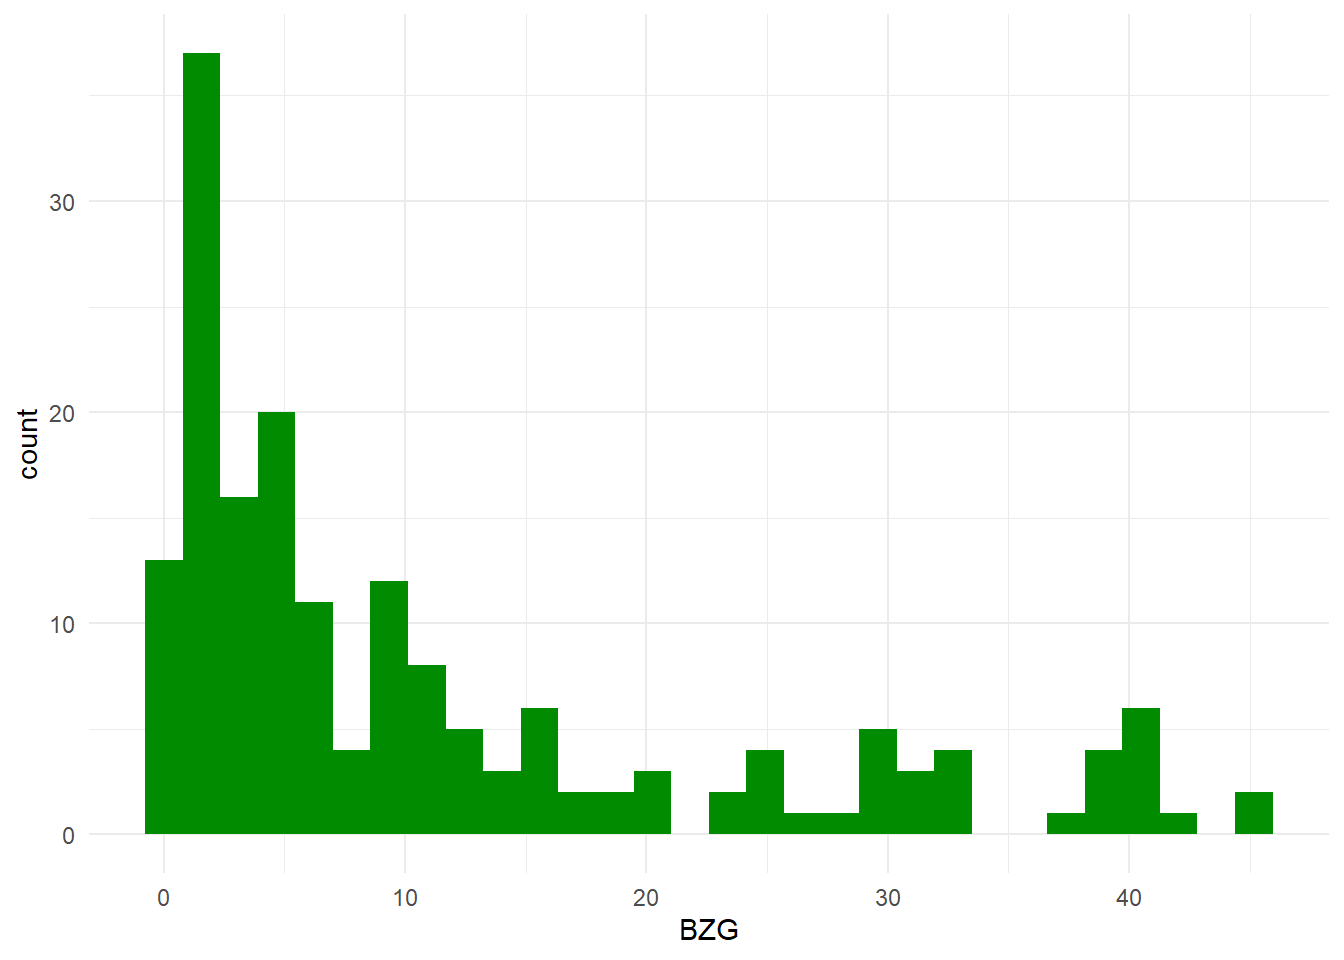
\includegraphics{0_Auswertung_files/figure-latex/unnamed-chunk-37-1.pdf}

\section{6. Verteilungen der
Soziodemografika}\label{verteilungen-der-soziodemografika}

\subsection{Geschlecht}\label{geschlecht}

\begin{Shaded}
\begin{Highlighting}[]
\NormalTok{raw4\_6 }\SpecialCharTok{\%\textgreater{}\%} 
  \FunctionTok{count}\NormalTok{(Geschlecht) }\SpecialCharTok{\%\textgreater{}\%} 
  \FunctionTok{mutate}\NormalTok{(}\AttributeTok{prob =}\NormalTok{ n}\SpecialCharTok{/}\FunctionTok{sum}\NormalTok{(n)) }\SpecialCharTok{\%\textgreater{}\%}
  \FunctionTok{round}\NormalTok{(}\DecValTok{2}\NormalTok{)}
\end{Highlighting}
\end{Shaded}

\begin{verbatim}
## # A tibble: 2 x 3
##   Geschlecht     n  prob
##        <dbl> <dbl> <dbl>
## 1          1    54  0.31
## 2          2   122  0.69
\end{verbatim}

\begin{quote}
1 = männlich 2 = weiblich
\end{quote}

\subsection{Alter}\label{alter}

\begin{Shaded}
\begin{Highlighting}[]
\NormalTok{raw4\_6 }\SpecialCharTok{\%\textgreater{}\%} 
  \FunctionTok{summarise}\NormalTok{(}\FunctionTok{mean}\NormalTok{(Alter, }\AttributeTok{na.rm=}\ConstantTok{TRUE}\NormalTok{),}
            \FunctionTok{median}\NormalTok{(Alter, }\AttributeTok{na.rm=}\ConstantTok{TRUE}\NormalTok{),}
         \FunctionTok{sd}\NormalTok{(Alter, }\AttributeTok{na.rm=}\ConstantTok{TRUE}\NormalTok{), }
         \FunctionTok{max}\NormalTok{(Alter, }\AttributeTok{na.rm =}\ConstantTok{TRUE}\NormalTok{),}
         \FunctionTok{min}\NormalTok{(Alter, }\AttributeTok{na.rm=}\ConstantTok{TRUE}\NormalTok{))}
\end{Highlighting}
\end{Shaded}

\begin{verbatim}
## # A tibble: 1 x 5
##   `mean(Alter, na.rm = TRUE)` median(Alter, na.rm = TRU~1 sd(Alter, na.rm = TR~2
##                         <dbl>                       <dbl>                  <dbl>
## 1                        40.3                          36                   13.4
## # i abbreviated names: 1: `median(Alter, na.rm = TRUE)`,
## #   2: `sd(Alter, na.rm = TRUE)`
## # i 2 more variables: `max(Alter, na.rm = TRUE)` <dbl>,
## #   `min(Alter, na.rm = TRUE)` <dbl>
\end{verbatim}

\begin{Shaded}
\begin{Highlighting}[]
\NormalTok{raw4\_6 }\SpecialCharTok{\%\textgreater{}\%} 
  \FunctionTok{filter}\NormalTok{(Alter }\SpecialCharTok{\textgreater{}} \DecValTok{60}\NormalTok{)}
\end{Highlighting}
\end{Shaded}

\begin{verbatim}
## # A tibble: 6 x 73
##      ID Alter Geschlecht Bildung Bildung_sonstig   BZG Beschaeftigungsart
##   <int> <dbl>      <dbl>   <dbl> <chr>           <dbl>              <dbl>
## 1     8    63          1       6 <NA>             41.5                  2
## 2    14    61          2       3 <NA>             23.2                  2
## 3    15    62          1       5 <NA>             44.5                  2
## 4    43    62          1       3 <NA>             45.7                  2
## 5   148    62          2       7 <NA>             15.7                  2
## 6   168    61          2       6 <NA>             11.3                  2
## # i 66 more variables: Arbeitszeitmodell <dbl>, Gehalt <dbl>,
## #   Position_im_Unternehmen <dbl>, Remotarbeit <dbl>, IS_K01 <dbl>,
## #   IS_K02 <dbl>, IS_K03 <dbl>, IS_K04 <dbl>, IS_E05 <dbl>, IS_E06 <dbl>,
## #   IS_E07 <dbl>, IS_E08 <dbl>, OC_A01 <dbl>, OC_A02 <dbl>, OC_A03 <dbl>,
## #   OC_A04 <dbl>, OC_A05 <dbl>, CPE_C01 <dbl>, CPE_C02 <dbl>, CPE_C03 <dbl>,
## #   CPE_C04 <dbl>, CPE_I05 <dbl>, CPE_I06 <dbl>, CPE_I07 <dbl>, CPE_I08 <dbl>,
## #   CPE_M09 <dbl>, CPE_M10 <dbl>, CPE_M11 <dbl>, CPE_M12 <dbl>, ...
\end{verbatim}

\subsubsection{visuelle Darstellung des
Alters}\label{visuelle-darstellung-des-alters}

\begin{Shaded}
\begin{Highlighting}[]
\NormalTok{mean\_value\_Alter }\OtherTok{\textless{}{-}} \FunctionTok{mean}\NormalTok{(raw4\_6}\SpecialCharTok{$}\NormalTok{Alter, }\AttributeTok{na.rm=}\ConstantTok{TRUE}\NormalTok{)}
\NormalTok{median\_value\_Alter }\OtherTok{\textless{}{-}} \FunctionTok{median}\NormalTok{(raw4\_6}\SpecialCharTok{$}\NormalTok{Alter, }\AttributeTok{na.rm=}\ConstantTok{TRUE}\NormalTok{)}
\NormalTok{sd\_value\_Alter }\OtherTok{\textless{}{-}} \FunctionTok{sd}\NormalTok{(raw4\_6}\SpecialCharTok{$}\NormalTok{Alter, }\AttributeTok{na.rm=}\ConstantTok{TRUE}\NormalTok{)}
\end{Highlighting}
\end{Shaded}

\begin{Shaded}
\begin{Highlighting}[]
\NormalTok{raw4\_6 }\SpecialCharTok{\%\textgreater{}\%} 
  \FunctionTok{filter}\NormalTok{(}\FunctionTok{is.na}\NormalTok{(Alter))}
\end{Highlighting}
\end{Shaded}

\begin{verbatim}
## # A tibble: 2 x 73
##      ID Alter Geschlecht Bildung Bildung_sonstig   BZG Beschaeftigungsart
##   <int> <dbl>      <dbl>   <dbl> <chr>           <dbl>              <dbl>
## 1   131    NA          2       7 <NA>               11                  2
## 2   142    NA          2       7 <NA>                7                  2
## # i 66 more variables: Arbeitszeitmodell <dbl>, Gehalt <dbl>,
## #   Position_im_Unternehmen <dbl>, Remotarbeit <dbl>, IS_K01 <dbl>,
## #   IS_K02 <dbl>, IS_K03 <dbl>, IS_K04 <dbl>, IS_E05 <dbl>, IS_E06 <dbl>,
## #   IS_E07 <dbl>, IS_E08 <dbl>, OC_A01 <dbl>, OC_A02 <dbl>, OC_A03 <dbl>,
## #   OC_A04 <dbl>, OC_A05 <dbl>, CPE_C01 <dbl>, CPE_C02 <dbl>, CPE_C03 <dbl>,
## #   CPE_C04 <dbl>, CPE_I05 <dbl>, CPE_I06 <dbl>, CPE_I07 <dbl>, CPE_I08 <dbl>,
## #   CPE_M09 <dbl>, CPE_M10 <dbl>, CPE_M11 <dbl>, CPE_M12 <dbl>, ...
\end{verbatim}

\begin{Shaded}
\begin{Highlighting}[]
\NormalTok{raw4\_6a }\OtherTok{\textless{}{-}}\NormalTok{ raw4\_6 }\SpecialCharTok{\%\textgreater{}\%} 
  \FunctionTok{drop\_na}\NormalTok{(Alter) }
\NormalTok{raw4\_6a}
\end{Highlighting}
\end{Shaded}

\begin{verbatim}
## # A tibble: 174 x 73
##       ID Alter Geschlecht Bildung Bildung_sonstig    BZG Beschaeftigungsart
##    <int> <dbl>      <dbl>   <dbl> <chr>            <dbl>              <dbl>
##  1     1    57          1       7 <NA>             0.833                  2
##  2     2    52          2       6 <NA>            26.7                    2
##  3     3    25          2       6 <NA>             2.25                   1
##  4     4    27          1       5 <NA>             4                      2
##  5     5    30          1       7 <NA>             6.75                   2
##  6     6    46          1       5 <NA>            15.9                    2
##  7     7    27          1       5 <NA>             6.75                   2
##  8     8    63          1       6 <NA>            41.5                    2
##  9     9    27          1       9 2. Staatsexamen  4                      2
## 10    10    26          1       4 <NA>             1.08                   1
## # i 164 more rows
## # i 66 more variables: Arbeitszeitmodell <dbl>, Gehalt <dbl>,
## #   Position_im_Unternehmen <dbl>, Remotarbeit <dbl>, IS_K01 <dbl>,
## #   IS_K02 <dbl>, IS_K03 <dbl>, IS_K04 <dbl>, IS_E05 <dbl>, IS_E06 <dbl>,
## #   IS_E07 <dbl>, IS_E08 <dbl>, OC_A01 <dbl>, OC_A02 <dbl>, OC_A03 <dbl>,
## #   OC_A04 <dbl>, OC_A05 <dbl>, CPE_C01 <dbl>, CPE_C02 <dbl>, CPE_C03 <dbl>,
## #   CPE_C04 <dbl>, CPE_I05 <dbl>, CPE_I06 <dbl>, CPE_I07 <dbl>, ...
\end{verbatim}

\begin{Shaded}
\begin{Highlighting}[]
\NormalTok{plot\_alter }\OtherTok{\textless{}{-}}\NormalTok{ raw4\_6a }\SpecialCharTok{\%\textgreater{}\%} 
  \FunctionTok{ggplot}\NormalTok{()}\SpecialCharTok{+}
  \FunctionTok{aes}\NormalTok{(}\AttributeTok{x=}\NormalTok{Alter)}\SpecialCharTok{+}
  \FunctionTok{geom\_histogram}\NormalTok{(}\AttributeTok{fill =} \StringTok{"grey71"}\NormalTok{,}
                 \AttributeTok{color =} \StringTok{"gray60"}\NormalTok{)}\SpecialCharTok{+}
  \FunctionTok{geom\_vline}\NormalTok{(}\AttributeTok{xintercept=}\NormalTok{mean\_value\_Alter , }\AttributeTok{color=}\StringTok{"turquoise3"}\NormalTok{, }\AttributeTok{size=}\DecValTok{2}\NormalTok{)}\SpecialCharTok{+}
  \FunctionTok{geom\_vline}\NormalTok{(}\AttributeTok{xintercept=}\NormalTok{mean\_value\_Alter}\SpecialCharTok{+}\NormalTok{sd\_value\_Alter, }\AttributeTok{color=}\StringTok{"coral1"}\NormalTok{, }\AttributeTok{size=}\FloatTok{1.5}\NormalTok{)}\SpecialCharTok{+}
  \FunctionTok{geom\_vline}\NormalTok{(}\AttributeTok{xintercept=}\NormalTok{mean\_value\_Alter}\SpecialCharTok{{-}}\NormalTok{sd\_value\_Alter, }\AttributeTok{color=}\StringTok{"coral1"}\NormalTok{, }\AttributeTok{size=}\FloatTok{1.5}\NormalTok{)}\SpecialCharTok{+}
  \FunctionTok{geom\_rect}\NormalTok{(}\AttributeTok{xmin =}\NormalTok{ mean\_value\_Alter }\SpecialCharTok{{-}}\NormalTok{ sd\_value\_Alter,}
            \AttributeTok{xmax=}\NormalTok{mean\_value\_Alter}\SpecialCharTok{+}\NormalTok{sd\_value\_Alter,}
            \AttributeTok{ymin=}\SpecialCharTok{{-}}\NormalTok{.}\DecValTok{1}\NormalTok{, }\AttributeTok{ymax=}\FloatTok{0.2}\NormalTok{, }\AttributeTok{fill=}\StringTok{"coral1"}\NormalTok{)}\SpecialCharTok{+}
  \FunctionTok{ylab}\NormalTok{(}\StringTok{"Anzahl"}\NormalTok{)}\SpecialCharTok{+}
  \FunctionTok{labs}\NormalTok{(}\AttributeTok{caption =} \StringTok{"N = 174,}
\StringTok{                  Türkis = Mittelwert, Rot = Standardabweichung"}\NormalTok{)}\SpecialCharTok{+}
  \FunctionTok{theme\_minimal}\NormalTok{()}
\end{Highlighting}
\end{Shaded}

\begin{verbatim}
## Warning: Using `size` aesthetic for lines was deprecated in ggplot2 3.4.0.
## i Please use `linewidth` instead.
## This warning is displayed once every 8 hours.
## Call `lifecycle::last_lifecycle_warnings()` to see where this warning was
## generated.
\end{verbatim}

\begin{Shaded}
\begin{Highlighting}[]
\NormalTok{plot\_alter}
\end{Highlighting}
\end{Shaded}

\begin{verbatim}
## `stat_bin()` using `bins = 30`. Pick better value with `binwidth`.
\end{verbatim}

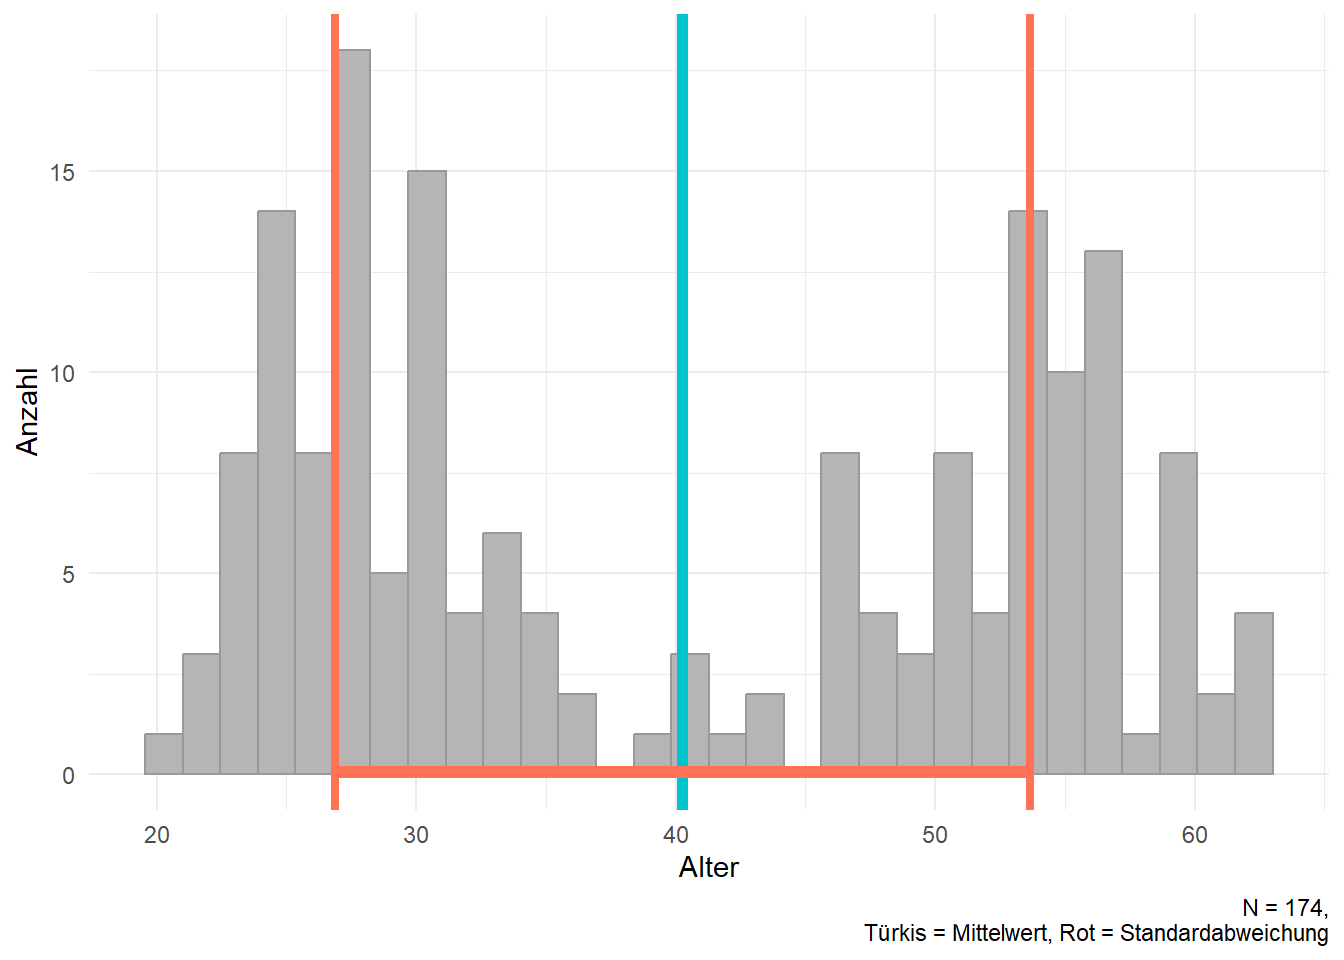
\includegraphics{0_Auswertung_files/figure-latex/unnamed-chunk-44-1.pdf}

\begin{Shaded}
\begin{Highlighting}[]
\FunctionTok{ggsave}\NormalTok{(}\AttributeTok{filename =} \StringTok{"Altersverteilung.png"}\NormalTok{, }\AttributeTok{plot =}\NormalTok{ plot\_alter, }\AttributeTok{width =} \DecValTok{8}\NormalTok{, }\AttributeTok{height =} \DecValTok{6}\NormalTok{, }\AttributeTok{dpi =} \DecValTok{300}\NormalTok{)}
\end{Highlighting}
\end{Shaded}

\begin{verbatim}
## `stat_bin()` using `bins = 30`. Pick better value with `binwidth`.
\end{verbatim}

\begin{Shaded}
\begin{Highlighting}[]
\FunctionTok{svg}\NormalTok{(}\StringTok{"Altersverteilung"}\NormalTok{, }\AttributeTok{width =} \DecValTok{7}\NormalTok{, }\AttributeTok{height =} \DecValTok{5}\NormalTok{)}
\FunctionTok{print}\NormalTok{(plot\_alter)}
\end{Highlighting}
\end{Shaded}

\begin{verbatim}
## `stat_bin()` using `bins = 30`. Pick better value with `binwidth`.
\end{verbatim}

\begin{Shaded}
\begin{Highlighting}[]
\FunctionTok{dev.off}\NormalTok{()}
\end{Highlighting}
\end{Shaded}

\begin{verbatim}
## pdf 
##   2
\end{verbatim}

\subsection{Bildung}\label{bildung}

\begin{Shaded}
\begin{Highlighting}[]
\NormalTok{raw4\_6 }\SpecialCharTok{\%\textgreater{}\%} 
  \FunctionTok{count}\NormalTok{(Bildung) }\SpecialCharTok{\%\textgreater{}\%} 
  \FunctionTok{mutate}\NormalTok{(}\AttributeTok{prob =}\NormalTok{ n}\SpecialCharTok{/}\FunctionTok{sum}\NormalTok{(n)) }\SpecialCharTok{\%\textgreater{}\%} 
  \FunctionTok{round}\NormalTok{(}\DecValTok{2}\NormalTok{)}
\end{Highlighting}
\end{Shaded}

\begin{verbatim}
## # A tibble: 8 x 3
##   Bildung     n  prob
##     <dbl> <dbl> <dbl>
## 1       2     7  0.04
## 2       3    20  0.11
## 3       4    19  0.11
## 4       5    32  0.18
## 5       6    53  0.3 
## 6       7    41  0.23
## 7       8     2  0.01
## 8       9     2  0.01
\end{verbatim}

\subsubsection{Visuelle Darstellung der
Bildung}\label{visuelle-darstellung-der-bildung}

\begin{Shaded}
\begin{Highlighting}[]
\NormalTok{raw4\_6 }\SpecialCharTok{\%\textgreater{}\%} 
  \FunctionTok{ggplot}\NormalTok{()}\SpecialCharTok{+}
  \FunctionTok{aes}\NormalTok{(}\AttributeTok{x=}\NormalTok{Bildung)}\SpecialCharTok{+}
  \FunctionTok{geom\_histogram}\NormalTok{(}\AttributeTok{fill =} \StringTok{"green4"}\NormalTok{)}\SpecialCharTok{+}
  \FunctionTok{theme\_minimal}\NormalTok{()}
\end{Highlighting}
\end{Shaded}

\begin{verbatim}
## `stat_bin()` using `bins = 30`. Pick better value with `binwidth`.
\end{verbatim}

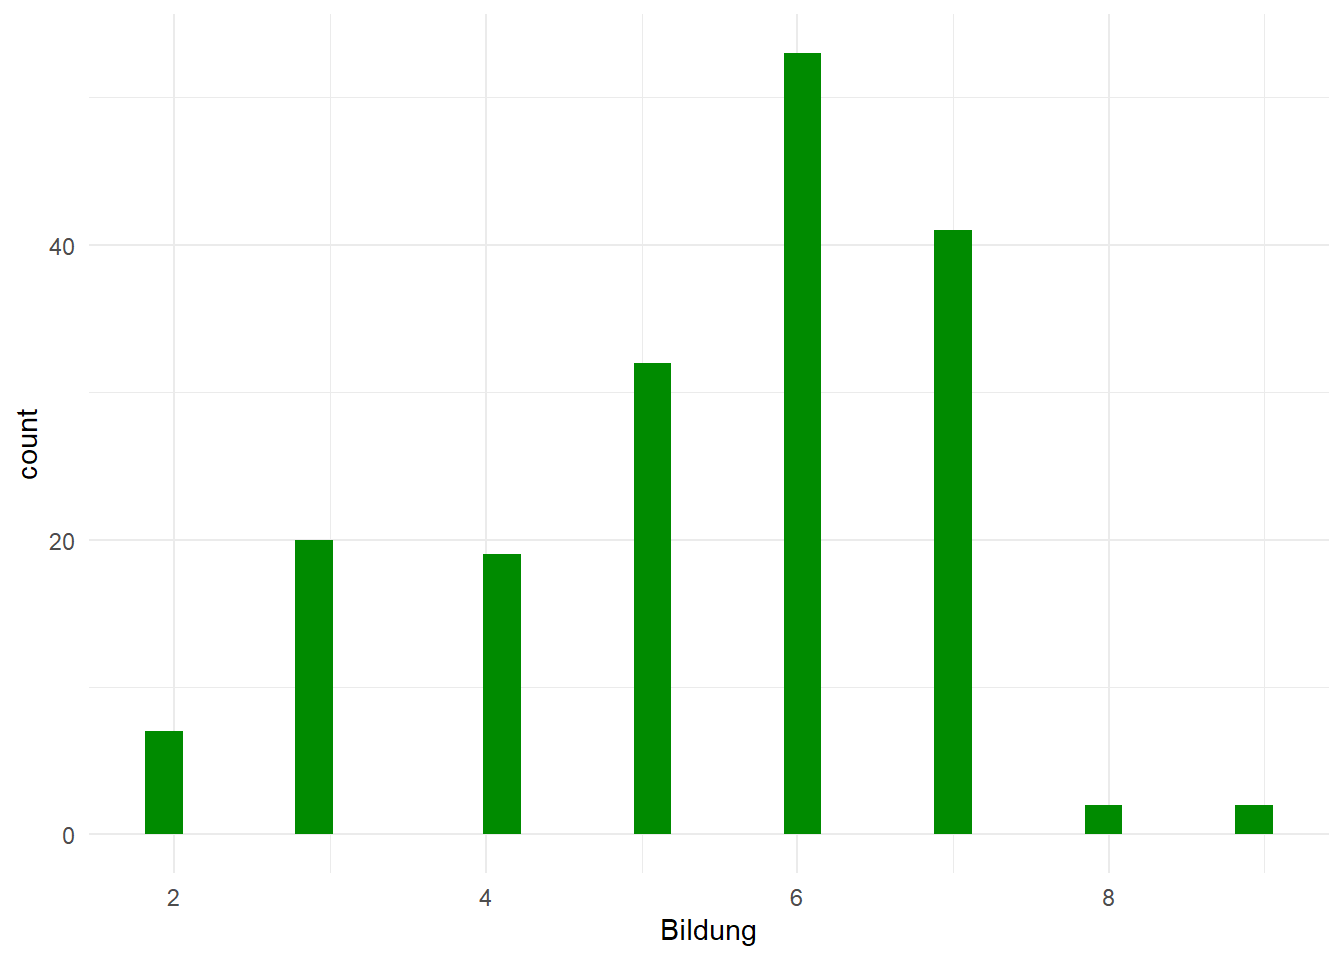
\includegraphics{0_Auswertung_files/figure-latex/unnamed-chunk-48-1.pdf}
\#\# Beschäftigungsart

\begin{Shaded}
\begin{Highlighting}[]
\NormalTok{raw4\_6 }\SpecialCharTok{\%\textgreater{}\%} 
  \FunctionTok{count}\NormalTok{(Beschaeftigungsart) }\SpecialCharTok{\%\textgreater{}\%} 
    \FunctionTok{mutate}\NormalTok{(}\AttributeTok{prob =}\NormalTok{ n}\SpecialCharTok{/}\FunctionTok{sum}\NormalTok{(n)) }\SpecialCharTok{\%\textgreater{}\%} 
  \FunctionTok{round}\NormalTok{(}\DecValTok{2}\NormalTok{)}
\end{Highlighting}
\end{Shaded}

\begin{verbatim}
## # A tibble: 2 x 3
##   Beschaeftigungsart     n  prob
##                <dbl> <dbl> <dbl>
## 1                  1    20  0.11
## 2                  2   156  0.89
\end{verbatim}

1 = befristet, 2 = unbefristet

\subsection{Arbeitszeitmodell =
Stunden/Woche}\label{arbeitszeitmodell-stundenwoche}

\begin{Shaded}
\begin{Highlighting}[]
\NormalTok{raw4\_6 }\SpecialCharTok{\%\textgreater{}\%} 
  \FunctionTok{summarise}\NormalTok{(}\AttributeTok{mean =} \FunctionTok{mean}\NormalTok{(Arbeitszeitmodell, }\AttributeTok{na.rm=}\ConstantTok{TRUE}\NormalTok{),}
            \AttributeTok{median =} \FunctionTok{median}\NormalTok{(Arbeitszeitmodell, }\AttributeTok{na.rm=}\ConstantTok{TRUE}\NormalTok{),}
         \AttributeTok{sd =} \FunctionTok{sd}\NormalTok{(Arbeitszeitmodell, }\AttributeTok{na.rm=}\ConstantTok{TRUE}\NormalTok{),}
         \AttributeTok{min =} \FunctionTok{min}\NormalTok{(Arbeitszeitmodell, }\AttributeTok{na.rm=}\ConstantTok{TRUE}\NormalTok{),}
         \AttributeTok{max =} \FunctionTok{max}\NormalTok{(Arbeitszeitmodell, }\AttributeTok{na.rm=}\ConstantTok{TRUE}\NormalTok{))}
\end{Highlighting}
\end{Shaded}

\begin{verbatim}
## # A tibble: 1 x 5
##    mean median    sd   min   max
##   <dbl>  <dbl> <dbl> <dbl> <dbl>
## 1  31.6     35  9.86     0    56
\end{verbatim}

\subsubsection{Visuelle Darstellung der verschiedenen
Arbeitsmodelle}\label{visuelle-darstellung-der-verschiedenen-arbeitsmodelle}

\begin{Shaded}
\begin{Highlighting}[]
\NormalTok{raw4\_6 }\SpecialCharTok{\%\textgreater{}\%} 
  \FunctionTok{ggplot}\NormalTok{()}\SpecialCharTok{+}
  \FunctionTok{aes}\NormalTok{(}\AttributeTok{x=}\NormalTok{Arbeitszeitmodell)}\SpecialCharTok{+}
  \FunctionTok{geom\_histogram}\NormalTok{(}\AttributeTok{fill =} \StringTok{"green4"}\NormalTok{)}\SpecialCharTok{+}
  \FunctionTok{theme\_minimal}\NormalTok{()}
\end{Highlighting}
\end{Shaded}

\begin{verbatim}
## `stat_bin()` using `bins = 30`. Pick better value with `binwidth`.
\end{verbatim}

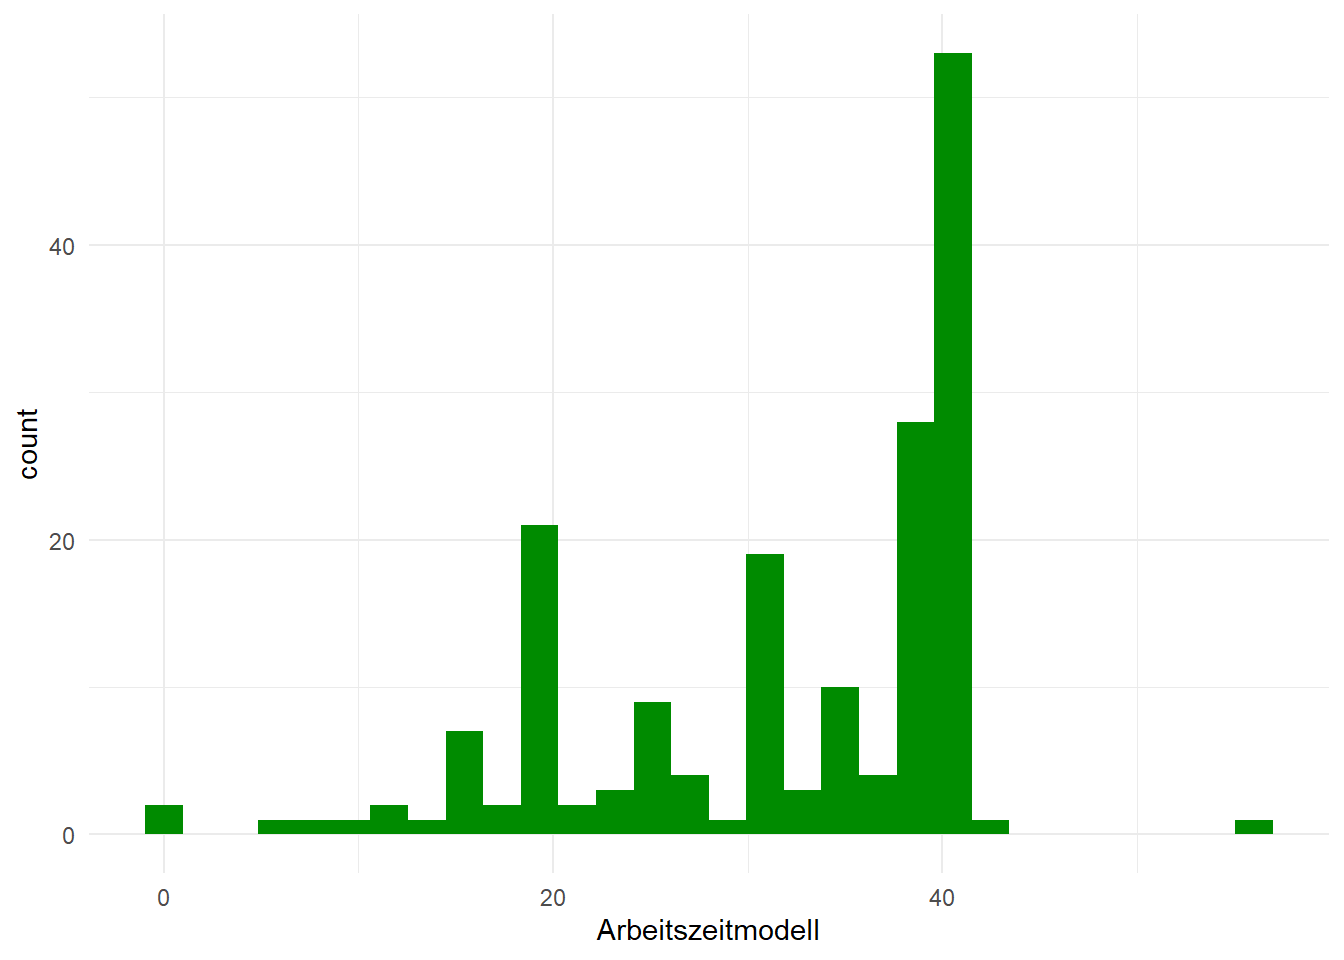
\includegraphics{0_Auswertung_files/figure-latex/unnamed-chunk-51-1.pdf}

\subsubsection{Arbeitszeitmodell Extremwerte
betrachten}\label{arbeitszeitmodell-extremwerte-betrachten}

\begin{Shaded}
\begin{Highlighting}[]
\NormalTok{raw4\_6 }\SpecialCharTok{\%\textgreater{}\%} 
  \FunctionTok{filter}\NormalTok{(Arbeitszeitmodell }\SpecialCharTok{\textless{}} \DecValTok{10} \SpecialCharTok{|}\NormalTok{ Arbeitszeitmodell }\SpecialCharTok{\textgreater{}} \DecValTok{45}\NormalTok{) }\SpecialCharTok{\%\textgreater{}\%} 
  \FunctionTok{arrange}\NormalTok{(}\FunctionTok{desc}\NormalTok{(Arbeitszeitmodell)) }\SpecialCharTok{\%\textgreater{}\%} 
  \FunctionTok{select}\NormalTok{(ID, Alter, Geschlecht, Bildung, Arbeitszeitmodell, }\FunctionTok{everything}\NormalTok{())}
\end{Highlighting}
\end{Shaded}

\begin{verbatim}
## # A tibble: 6 x 73
##      ID Alter Geschlecht Bildung Arbeitszeitmodell Bildung_sonstig    BZG
##   <int> <dbl>      <dbl>   <dbl>             <dbl> <chr>            <dbl>
## 1    93    29          1       5              56   <NA>             2.67 
## 2    47    24          1       6               9   <NA>             5    
## 3    57    23          1       6               7.5 <NA>             0.583
## 4    66    23          1       4               5   <NA>             0.583
## 5   124    46          1       7               0   <NA>             3.75 
## 6   155    59          2       6               0   <NA>            39.8  
## # i 66 more variables: Beschaeftigungsart <dbl>, Gehalt <dbl>,
## #   Position_im_Unternehmen <dbl>, Remotarbeit <dbl>, IS_K01 <dbl>,
## #   IS_K02 <dbl>, IS_K03 <dbl>, IS_K04 <dbl>, IS_E05 <dbl>, IS_E06 <dbl>,
## #   IS_E07 <dbl>, IS_E08 <dbl>, OC_A01 <dbl>, OC_A02 <dbl>, OC_A03 <dbl>,
## #   OC_A04 <dbl>, OC_A05 <dbl>, CPE_C01 <dbl>, CPE_C02 <dbl>, CPE_C03 <dbl>,
## #   CPE_C04 <dbl>, CPE_I05 <dbl>, CPE_I06 <dbl>, CPE_I07 <dbl>, CPE_I08 <dbl>,
## #   CPE_M09 <dbl>, CPE_M10 <dbl>, CPE_M11 <dbl>, CPE_M12 <dbl>, ...
\end{verbatim}

\subsection{Gehalt}\label{gehalt}

\begin{Shaded}
\begin{Highlighting}[]
\NormalTok{raw4\_6 }\SpecialCharTok{\%\textgreater{}\%} 
  \FunctionTok{count}\NormalTok{(Gehalt) }\SpecialCharTok{\%\textgreater{}\%} 
  \FunctionTok{mutate}\NormalTok{(}\AttributeTok{prob =}\NormalTok{ n}\SpecialCharTok{/}\FunctionTok{sum}\NormalTok{(n)) }\SpecialCharTok{\%\textgreater{}\%} 
  \FunctionTok{round}\NormalTok{(}\DecValTok{2}\NormalTok{)}
\end{Highlighting}
\end{Shaded}

\begin{verbatim}
## # A tibble: 8 x 3
##   Gehalt     n  prob
##    <dbl> <dbl> <dbl>
## 1      1    14  0.08
## 2      2    54  0.31
## 3      3    56  0.32
## 4      4    27  0.15
## 5      5     7  0.04
## 6      6     6  0.03
## 7      7    10  0.06
## 8     NA     2  0.01
\end{verbatim}

\subsubsection{Visuelle Darstellung des
Gehalts}\label{visuelle-darstellung-des-gehalts}

\begin{Shaded}
\begin{Highlighting}[]
\NormalTok{raw4\_6 }\SpecialCharTok{\%\textgreater{}\%} 
  \FunctionTok{ggplot}\NormalTok{()}\SpecialCharTok{+}
  \FunctionTok{aes}\NormalTok{(}\AttributeTok{x=}\NormalTok{Gehalt)}\SpecialCharTok{+}
  \FunctionTok{geom\_histogram}\NormalTok{(}\AttributeTok{fill =} \StringTok{"green4"}\NormalTok{)}\SpecialCharTok{+}
  \FunctionTok{theme\_minimal}\NormalTok{()}
\end{Highlighting}
\end{Shaded}

\begin{verbatim}
## `stat_bin()` using `bins = 30`. Pick better value with `binwidth`.
\end{verbatim}

\begin{verbatim}
## Warning: Removed 2 rows containing non-finite values (`stat_bin()`).
\end{verbatim}

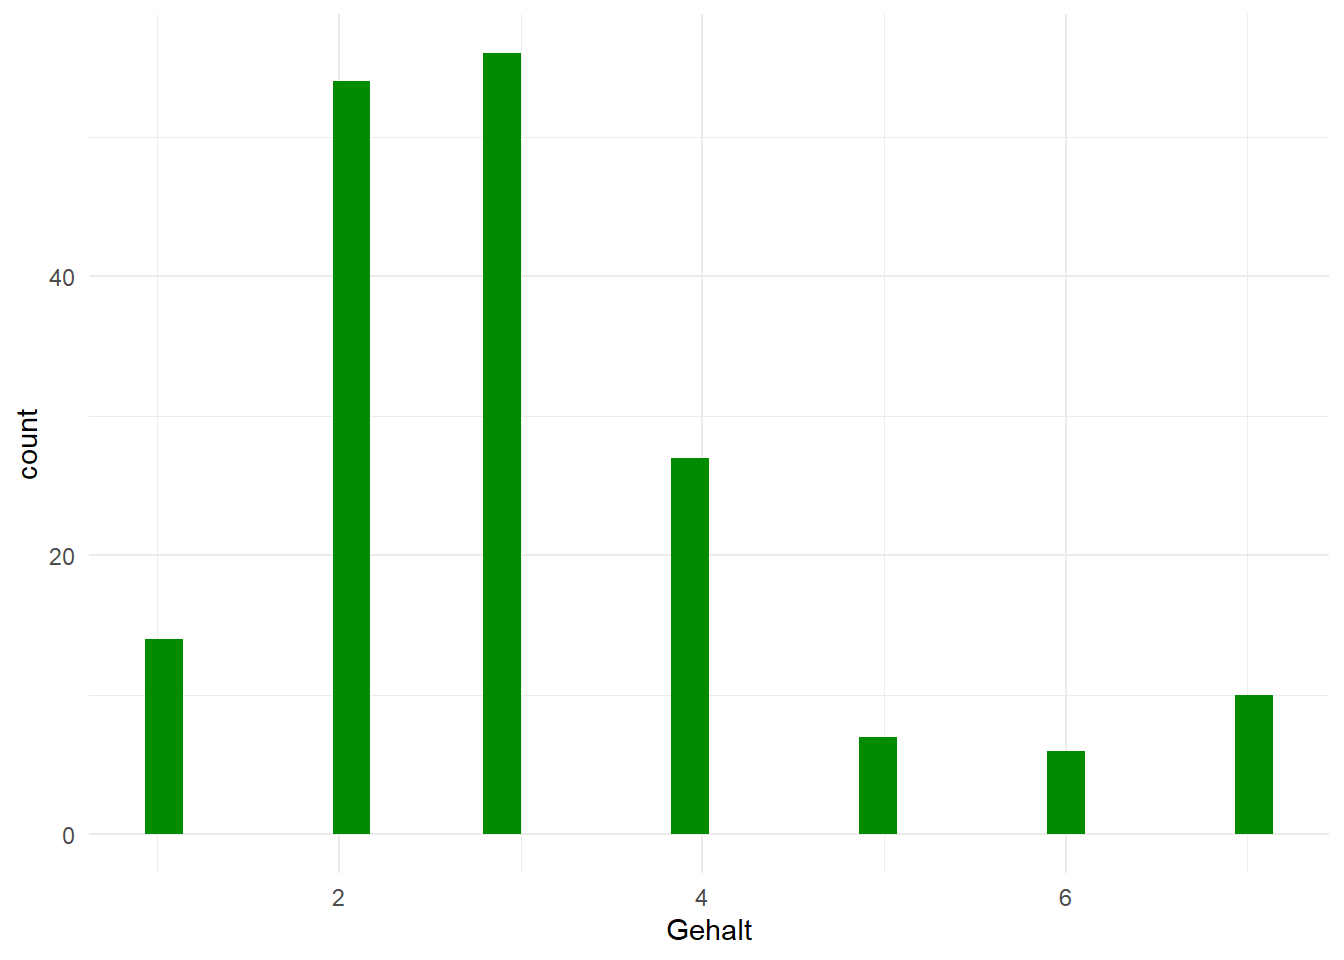
\includegraphics{0_Auswertung_files/figure-latex/unnamed-chunk-54-1.pdf}
\textgreater{} Nach Absprache mit Frau Sende werden die Gehaltsstufen
5-7 in einer Stufe zusammengefasst!

\paragraph{Gehaltsstufen 5-7
zusammenfassen}\label{gehaltsstufen-5-7-zusammenfassen}

\begin{Shaded}
\begin{Highlighting}[]
\NormalTok{raw4\_7 }\OtherTok{\textless{}{-}}\NormalTok{ raw4\_6 }\SpecialCharTok{\%\textgreater{}\%} 
  \FunctionTok{mutate}\NormalTok{(}\AttributeTok{Gehalt\_n =} \FunctionTok{case\_when}\NormalTok{(}
\NormalTok{    Gehalt }\SpecialCharTok{==} \DecValTok{1} \SpecialCharTok{\textasciitilde{}} \DecValTok{1}\NormalTok{,}
\NormalTok{    Gehalt }\SpecialCharTok{==} \DecValTok{2} \SpecialCharTok{\textasciitilde{}} \DecValTok{2}\NormalTok{,}
\NormalTok{    Gehalt }\SpecialCharTok{==} \DecValTok{3} \SpecialCharTok{\textasciitilde{}} \DecValTok{3}\NormalTok{,}
\NormalTok{    Gehalt }\SpecialCharTok{==} \DecValTok{4} \SpecialCharTok{\textasciitilde{}} \DecValTok{4}\NormalTok{,}
\NormalTok{    Gehalt }\SpecialCharTok{==} \DecValTok{5} \SpecialCharTok{\textasciitilde{}} \DecValTok{5}\NormalTok{,}
\NormalTok{    Gehalt }\SpecialCharTok{==} \DecValTok{6} \SpecialCharTok{\textasciitilde{}} \DecValTok{5}\NormalTok{,}
\NormalTok{    Gehalt }\SpecialCharTok{==} \DecValTok{7} \SpecialCharTok{\textasciitilde{}} \DecValTok{5}\NormalTok{))}
\end{Highlighting}
\end{Shaded}

\begin{Shaded}
\begin{Highlighting}[]
\NormalTok{raw4\_7 }\SpecialCharTok{\%\textgreater{}\%} 
  \FunctionTok{select}\NormalTok{(Gehalt, Gehalt\_n) }\SpecialCharTok{\%\textgreater{}\%} 
  \FunctionTok{arrange}\NormalTok{(}\FunctionTok{desc}\NormalTok{(Gehalt))}
\end{Highlighting}
\end{Shaded}

\begin{verbatim}
## # A tibble: 176 x 2
##    Gehalt Gehalt_n
##     <dbl>    <dbl>
##  1      7        5
##  2      7        5
##  3      7        5
##  4      7        5
##  5      7        5
##  6      7        5
##  7      7        5
##  8      7        5
##  9      7        5
## 10      7        5
## # i 166 more rows
\end{verbatim}

\begin{Shaded}
\begin{Highlighting}[]
\NormalTok{raw4\_8 }\OtherTok{\textless{}{-}}\NormalTok{ raw4\_7 }\SpecialCharTok{\%\textgreater{}\%} 
  \FunctionTok{select}\NormalTok{(}\SpecialCharTok{{-}}\NormalTok{Gehalt) }\SpecialCharTok{\%\textgreater{}\%} 
  \FunctionTok{select}\NormalTok{(ID, Alter, Geschlecht, Bildung, Bildung\_sonstig, BZG, Beschaeftigungsart, Arbeitszeitmodell, Gehalt\_n, Position\_im\_Unternehmen, Remotarbeit, }\FunctionTok{everything}\NormalTok{())}
\end{Highlighting}
\end{Shaded}

\begin{Shaded}
\begin{Highlighting}[]
\NormalTok{raw4\_8 }\SpecialCharTok{\%\textgreater{}\%} 
  \FunctionTok{ggplot}\NormalTok{()}\SpecialCharTok{+}
  \FunctionTok{aes}\NormalTok{(}\AttributeTok{x=}\NormalTok{Gehalt\_n)}\SpecialCharTok{+}
  \FunctionTok{geom\_histogram}\NormalTok{(}\AttributeTok{fill =} \StringTok{"green4"}\NormalTok{)}\SpecialCharTok{+}
  \FunctionTok{theme\_minimal}\NormalTok{()}
\end{Highlighting}
\end{Shaded}

\begin{verbatim}
## `stat_bin()` using `bins = 30`. Pick better value with `binwidth`.
\end{verbatim}

\begin{verbatim}
## Warning: Removed 2 rows containing non-finite values (`stat_bin()`).
\end{verbatim}

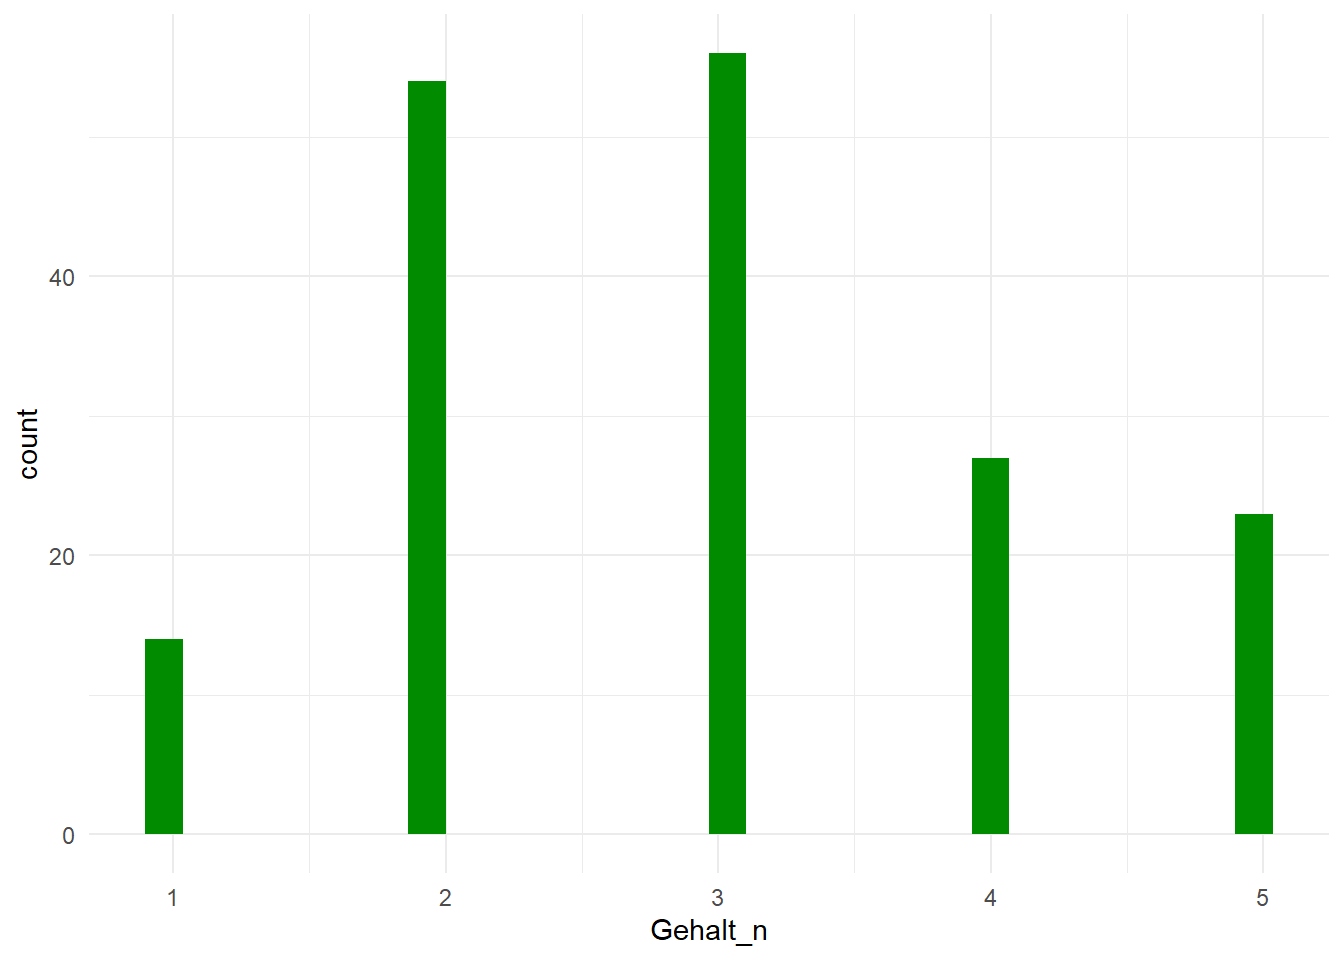
\includegraphics{0_Auswertung_files/figure-latex/unnamed-chunk-58-1.pdf}

\subsection{Position im Unternehmen}\label{position-im-unternehmen}

\begin{Shaded}
\begin{Highlighting}[]
\NormalTok{raw4\_8 }\SpecialCharTok{\%\textgreater{}\%} 
  \FunctionTok{count}\NormalTok{(Position\_im\_Unternehmen) }\SpecialCharTok{\%\textgreater{}\%} 
  \FunctionTok{mutate}\NormalTok{(}\AttributeTok{prob =}\NormalTok{ n}\SpecialCharTok{/}\FunctionTok{sum}\NormalTok{(n)) }\SpecialCharTok{\%\textgreater{}\%} 
  \FunctionTok{round}\NormalTok{(}\DecValTok{2}\NormalTok{)}
\end{Highlighting}
\end{Shaded}

\begin{verbatim}
## # A tibble: 4 x 3
##   Position_im_Unternehmen     n  prob
##                     <dbl> <dbl> <dbl>
## 1                       1   139  0.79
## 2                       2    20  0.11
## 3                       3    12  0.07
## 4                       4     5  0.03
\end{verbatim}

\subsubsection{Visuelle Darstellung der Position im
Unternehmen}\label{visuelle-darstellung-der-position-im-unternehmen}

\begin{Shaded}
\begin{Highlighting}[]
\NormalTok{raw4\_8 }\SpecialCharTok{\%\textgreater{}\%} 
  \FunctionTok{ggplot}\NormalTok{()}\SpecialCharTok{+}
  \FunctionTok{aes}\NormalTok{(}\AttributeTok{x=}\NormalTok{Position\_im\_Unternehmen)}\SpecialCharTok{+}
  \FunctionTok{geom\_histogram}\NormalTok{(}\AttributeTok{fill =} \StringTok{"green4"}\NormalTok{)}\SpecialCharTok{+}
  \FunctionTok{theme\_minimal}\NormalTok{()}
\end{Highlighting}
\end{Shaded}

\begin{verbatim}
## `stat_bin()` using `bins = 30`. Pick better value with `binwidth`.
\end{verbatim}

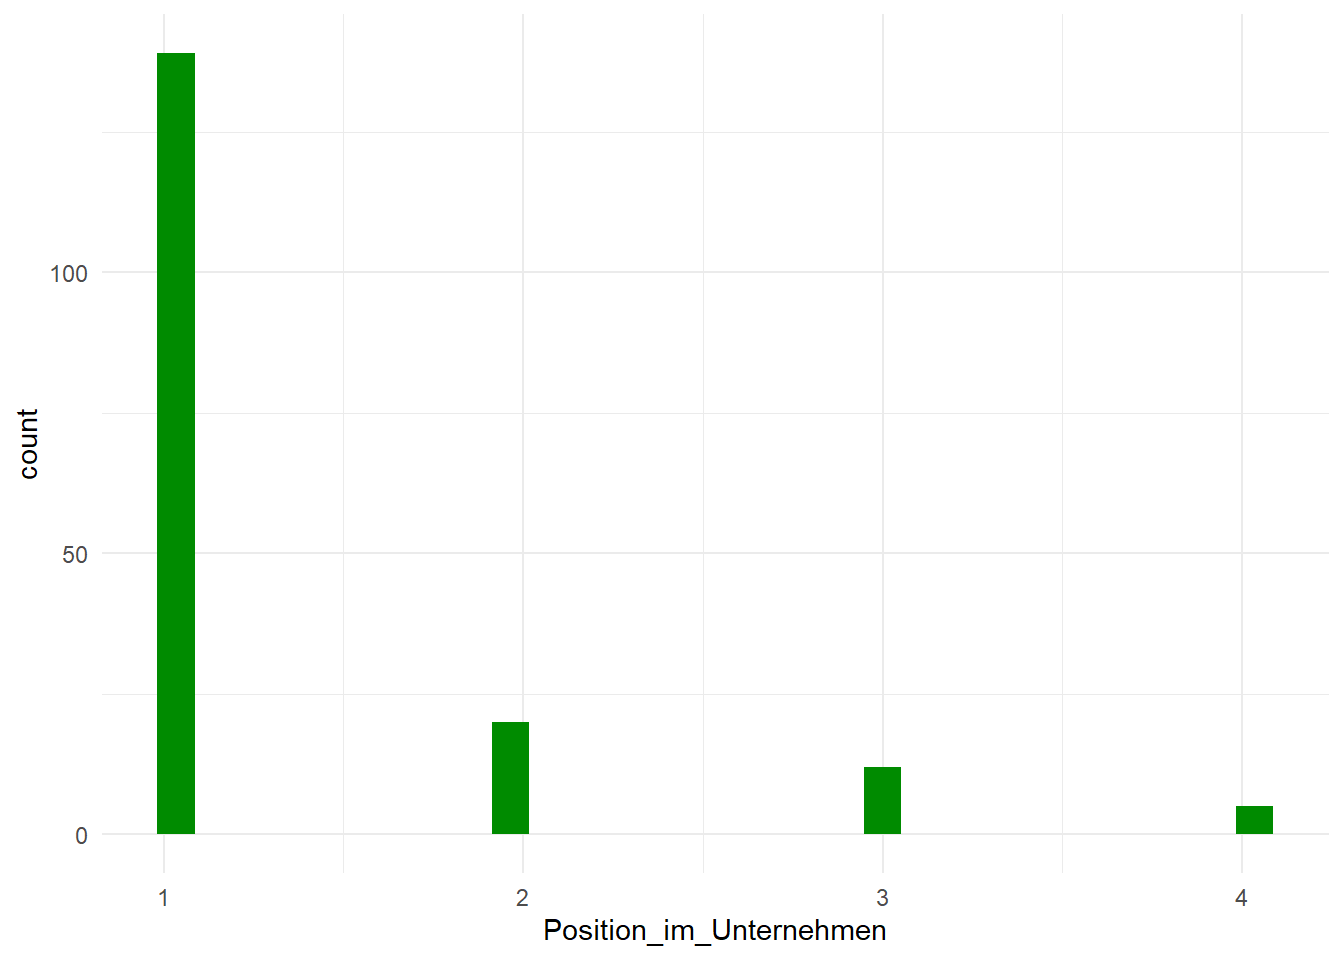
\includegraphics{0_Auswertung_files/figure-latex/unnamed-chunk-60-1.pdf}

\subsection{Remotearbeit}\label{remotearbeit}

\begin{Shaded}
\begin{Highlighting}[]
\NormalTok{raw4\_8 }\SpecialCharTok{\%\textgreater{}\%} 
  \FunctionTok{count}\NormalTok{(Remotarbeit) }\SpecialCharTok{\%\textgreater{}\%} 
  \FunctionTok{mutate}\NormalTok{(}\AttributeTok{prob =}\NormalTok{ n}\SpecialCharTok{/}\FunctionTok{sum}\NormalTok{(n)) }\SpecialCharTok{\%\textgreater{}\%} 
  \FunctionTok{round}\NormalTok{(}\DecValTok{2}\NormalTok{)}
\end{Highlighting}
\end{Shaded}

\begin{verbatim}
## # A tibble: 6 x 3
##   Remotarbeit     n  prob
##         <dbl> <dbl> <dbl>
## 1           1    85  0.48
## 2           2    26  0.15
## 3           3    26  0.15
## 4           4    22  0.12
## 5           5     9  0.05
## 6           6     8  0.05
\end{verbatim}

\subsubsection{Visuelle Darstellung der
Remotearbeit}\label{visuelle-darstellung-der-remotearbeit}

\begin{Shaded}
\begin{Highlighting}[]
\NormalTok{raw4\_8 }\SpecialCharTok{\%\textgreater{}\%} 
  \FunctionTok{ggplot}\NormalTok{()}\SpecialCharTok{+}
  \FunctionTok{aes}\NormalTok{(}\AttributeTok{x=}\NormalTok{Remotarbeit)}\SpecialCharTok{+}
  \FunctionTok{geom\_bar}\NormalTok{(}\AttributeTok{fill =} \StringTok{"green4"}\NormalTok{)}\SpecialCharTok{+}
  \FunctionTok{theme\_minimal}\NormalTok{()}
\end{Highlighting}
\end{Shaded}

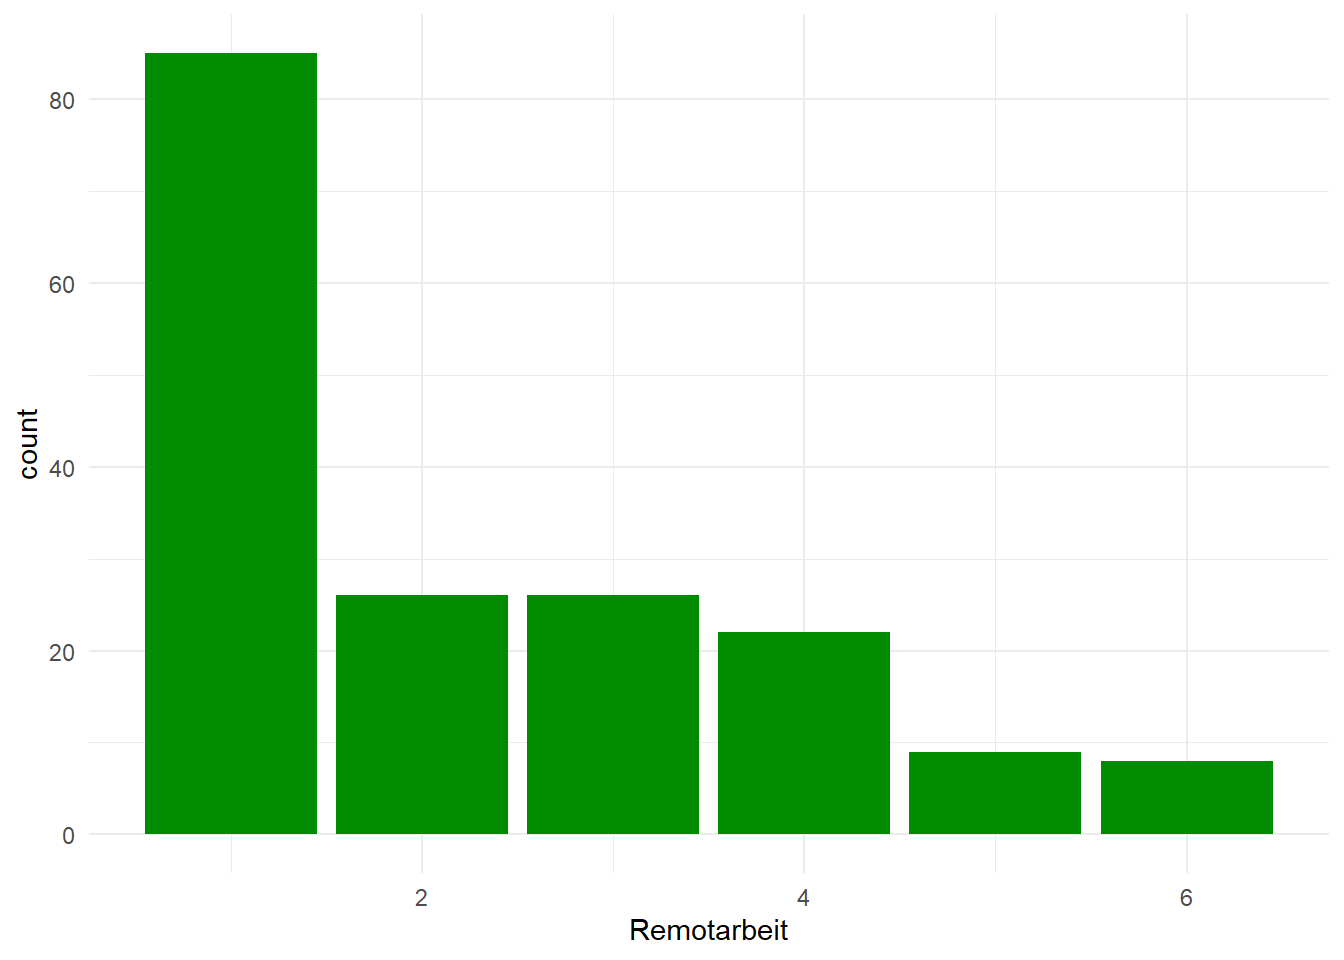
\includegraphics{0_Auswertung_files/figure-latex/unnamed-chunk-62-1.pdf}

\section{\texorpdfstring{7. Datensatz \texttt{raw\_8}
zwischenspeichern}{7. Datensatz raw\_8 zwischenspeichern}}\label{datensatz-raw_8-zwischenspeichern}

\begin{Shaded}
\begin{Highlighting}[]
\FunctionTok{write.csv}\NormalTok{(raw4\_8, }\AttributeTok{file=}\StringTok{"raw4.csv"}\NormalTok{)}
\end{Highlighting}
\end{Shaded}

\section{8. Cronbachs Alpha berechnen}\label{cronbachs-alpha-berechnen}

\subsection{Irritation}\label{irritation}

\begin{Shaded}
\begin{Highlighting}[]
\NormalTok{psych}\SpecialCharTok{::}\FunctionTok{alpha}\NormalTok{(}\FunctionTok{subset}\NormalTok{(raw4\_8, }\AttributeTok{select=}\FunctionTok{c}\NormalTok{(IS\_K01}\SpecialCharTok{:}\NormalTok{IS\_E08)), }\AttributeTok{check.keys=}\ConstantTok{TRUE}\NormalTok{)}
\end{Highlighting}
\end{Shaded}

\begin{verbatim}
## 
## Reliability analysis   
## Call: psych::alpha(x = subset(raw4_8, select = c(IS_K01:IS_E08)), check.keys = TRUE)
## 
##   raw_alpha std.alpha G6(smc) average_r S/N   ase mean  sd median_r
##       0.86      0.86    0.89      0.44 6.3 0.016  3.2 1.2     0.42
## 
##     95% confidence boundaries 
##          lower alpha upper
## Feldt     0.83  0.86  0.89
## Duhachek  0.83  0.86  0.89
## 
##  Reliability if an item is dropped:
##        raw_alpha std.alpha G6(smc) average_r S/N alpha se var.r med.r
## IS_K01      0.83      0.84    0.86      0.42 5.1    0.020 0.026  0.41
## IS_K02      0.84      0.85    0.87      0.44 5.6    0.018 0.021  0.43
## IS_K03      0.85      0.85    0.88      0.46 5.9    0.017 0.028  0.43
## IS_K04      0.85      0.85    0.87      0.44 5.6    0.018 0.023  0.43
## IS_E05      0.85      0.85    0.88      0.44 5.5    0.018 0.037  0.40
## IS_E06      0.85      0.85    0.88      0.44 5.5    0.018 0.033  0.41
## IS_E07      0.85      0.85    0.87      0.45 5.8    0.017 0.028  0.44
## IS_E08      0.84      0.84    0.87      0.42 5.1    0.020 0.035  0.37
## 
##  Item statistics 
##          n raw.r std.r r.cor r.drop mean  sd
## IS_K01 176  0.80  0.79  0.77   0.72  3.5 1.8
## IS_K02 176  0.72  0.70  0.68   0.61  4.2 1.8
## IS_K03 176  0.63  0.66  0.60   0.53  2.7 1.5
## IS_K04 176  0.72  0.70  0.67   0.61  3.4 2.0
## IS_E05 176  0.71  0.72  0.66   0.60  2.7 1.7
## IS_E06 176  0.69  0.71  0.66   0.59  3.1 1.7
## IS_E07 176  0.65  0.67  0.62   0.53  3.4 1.7
## IS_E08 176  0.77  0.78  0.73   0.70  2.6 1.6
## 
## Non missing response frequency for each item
##           1    2    3    4    5    6    7 miss
## IS_K01 0.15 0.23 0.20 0.10 0.15 0.10 0.07    0
## IS_K02 0.06 0.18 0.15 0.09 0.25 0.18 0.10    0
## IS_K03 0.22 0.34 0.23 0.08 0.10 0.02 0.03    0
## IS_K04 0.19 0.22 0.16 0.06 0.15 0.13 0.07    0
## IS_E05 0.34 0.23 0.14 0.09 0.11 0.06 0.02    0
## IS_E06 0.19 0.25 0.18 0.12 0.18 0.04 0.03    0
## IS_E07 0.15 0.24 0.18 0.11 0.22 0.07 0.03    0
## IS_E08 0.32 0.22 0.22 0.09 0.10 0.03 0.02    0
\end{verbatim}

\subsection{CPE}\label{cpe}

\begin{Shaded}
\begin{Highlighting}[]
\NormalTok{psych}\SpecialCharTok{::}\FunctionTok{alpha}\NormalTok{(}\FunctionTok{subset}\NormalTok{(raw4\_8, }\AttributeTok{select=}\FunctionTok{c}\NormalTok{(CPE\_C01}\SpecialCharTok{:}\NormalTok{CPE\_E16)), }\AttributeTok{check.keys=}\ConstantTok{TRUE}\NormalTok{)}
\end{Highlighting}
\end{Shaded}

\begin{verbatim}
## 
## Reliability analysis   
## Call: psych::alpha(x = subset(raw4_8, select = c(CPE_C01:CPE_E16)), 
##     check.keys = TRUE)
## 
##   raw_alpha std.alpha G6(smc) average_r S/N    ase mean  sd median_r
##       0.95      0.95    0.96      0.55  20 0.0053  4.8 1.1     0.57
## 
##     95% confidence boundaries 
##          lower alpha upper
## Feldt     0.94  0.95  0.96
## Duhachek  0.94  0.95  0.96
## 
##  Reliability if an item is dropped:
##         raw_alpha std.alpha G6(smc) average_r S/N alpha se  var.r med.r
## CPE_C01      0.95      0.95    0.96      0.54  18   0.0058 0.0139  0.57
## CPE_C02      0.95      0.95    0.96      0.56  19   0.0055 0.0131  0.57
## CPE_C03      0.95      0.95    0.96      0.54  18   0.0058 0.0140  0.57
## CPE_C04      0.95      0.95    0.96      0.54  18   0.0058 0.0134  0.57
## CPE_I05      0.95      0.95    0.96      0.54  18   0.0058 0.0140  0.57
## CPE_I06      0.95      0.95    0.96      0.55  18   0.0057 0.0143  0.57
## CPE_I07      0.95      0.95    0.96      0.58  21   0.0051 0.0049  0.58
## CPE_I08      0.95      0.95    0.96      0.55  18   0.0056 0.0144  0.57
## CPE_M09      0.95      0.95    0.96      0.55  18   0.0057 0.0135  0.57
## CPE_M10      0.95      0.95    0.96      0.55  18   0.0057 0.0134  0.57
## CPE_M11      0.95      0.95    0.96      0.55  18   0.0057 0.0138  0.57
## CPE_M12      0.95      0.95    0.96      0.55  18   0.0057 0.0141  0.57
## CPE_E13      0.95      0.95    0.95      0.54  18   0.0059 0.0131  0.56
## CPE_E14      0.95      0.95    0.96      0.55  18   0.0058 0.0133  0.57
## CPE_E15      0.95      0.95    0.96      0.55  18   0.0057 0.0140  0.57
## CPE_E16      0.95      0.95    0.96      0.56  19   0.0055 0.0135  0.57
## 
##  Item statistics 
##           n raw.r std.r r.cor r.drop mean  sd
## CPE_C01 176  0.82  0.81  0.80   0.78  4.9 1.5
## CPE_C02 176  0.71  0.70  0.68   0.66  4.9 1.6
## CPE_C03 176  0.80  0.80  0.79   0.77  5.1 1.5
## CPE_C04 176  0.81  0.80  0.79   0.77  4.7 1.5
## CPE_I05 176  0.81  0.82  0.81   0.78  5.1 1.4
## CPE_I06 176  0.78  0.78  0.77   0.75  4.8 1.4
## CPE_I07 176  0.46  0.46  0.41   0.39  5.3 1.4
## CPE_I08 176  0.76  0.76  0.74   0.72  4.8 1.5
## CPE_M09 176  0.78  0.78  0.76   0.74  4.2 1.6
## CPE_M10 176  0.77  0.77  0.76   0.73  4.7 1.6
## CPE_M11 175  0.78  0.78  0.77   0.75  4.6 1.4
## CPE_M12 176  0.76  0.76  0.75   0.72  5.2 1.4
## CPE_E13 176  0.84  0.84  0.83   0.81  4.6 1.6
## CPE_E14 176  0.80  0.80  0.79   0.77  4.9 1.5
## CPE_E15 176  0.79  0.79  0.78   0.76  4.9 1.4
## CPE_E16 176  0.71  0.70  0.68   0.66  4.8 1.6
## 
## Non missing response frequency for each item
##            1    2    3    4    5    6    7 miss
## CPE_C01 0.03 0.06 0.13 0.11 0.29 0.26 0.13 0.00
## CPE_C02 0.04 0.06 0.11 0.13 0.26 0.25 0.15 0.00
## CPE_C03 0.03 0.02 0.09 0.18 0.24 0.27 0.16 0.00
## CPE_C04 0.04 0.05 0.14 0.14 0.29 0.26 0.09 0.00
## CPE_I05 0.02 0.02 0.10 0.22 0.19 0.31 0.15 0.00
## CPE_I06 0.03 0.03 0.12 0.20 0.27 0.26 0.09 0.00
## CPE_I07 0.01 0.03 0.06 0.16 0.20 0.32 0.21 0.00
## CPE_I08 0.02 0.06 0.15 0.17 0.22 0.27 0.11 0.00
## CPE_M09 0.08 0.07 0.18 0.21 0.22 0.19 0.05 0.00
## CPE_M10 0.05 0.06 0.10 0.17 0.27 0.25 0.10 0.00
## CPE_M11 0.02 0.03 0.16 0.21 0.31 0.21 0.07 0.01
## CPE_M12 0.02 0.03 0.08 0.16 0.25 0.31 0.16 0.00
## CPE_E13 0.05 0.05 0.15 0.18 0.27 0.18 0.13 0.00
## CPE_E14 0.03 0.03 0.12 0.16 0.25 0.28 0.12 0.00
## CPE_E15 0.02 0.05 0.11 0.15 0.27 0.30 0.11 0.00
## CPE_E16 0.05 0.06 0.10 0.15 0.27 0.25 0.12 0.00
\end{verbatim}

\subsection{PS}\label{ps}

\begin{Shaded}
\begin{Highlighting}[]
\NormalTok{psych}\SpecialCharTok{::}\FunctionTok{alpha}\NormalTok{(}\FunctionTok{subset}\NormalTok{(raw4\_8, }\AttributeTok{select=}\FunctionTok{c}\NormalTok{(PS\_01}\SpecialCharTok{:}\NormalTok{PS\_07)), }\AttributeTok{check.keys=}\ConstantTok{TRUE}\NormalTok{)}
\end{Highlighting}
\end{Shaded}

\begin{verbatim}
## 
## Reliability analysis   
## Call: psych::alpha(x = subset(raw4_8, select = c(PS_01:PS_07)), check.keys = TRUE)
## 
##   raw_alpha std.alpha G6(smc) average_r S/N   ase mean  sd median_r
##       0.88      0.88    0.87      0.52 7.5 0.014  5.4 1.2     0.53
## 
##     95% confidence boundaries 
##          lower alpha upper
## Feldt     0.85  0.88  0.90
## Duhachek  0.85  0.88  0.91
## 
##  Reliability if an item is dropped:
##       raw_alpha std.alpha G6(smc) average_r S/N alpha se  var.r med.r
## PS_01      0.85      0.85    0.84      0.49 5.9    0.017 0.0055  0.49
## PS_02      0.88      0.88    0.86      0.55 7.2    0.014 0.0030  0.56
## PS_03      0.85      0.86    0.84      0.50 6.0    0.017 0.0060  0.51
## PS_04      0.86      0.86    0.85      0.51 6.3    0.016 0.0058  0.53
## PS_05      0.87      0.87    0.85      0.52 6.6    0.016 0.0043  0.53
## PS_06      0.87      0.87    0.86      0.53 6.7    0.016 0.0057  0.56
## PS_07      0.86      0.87    0.85      0.52 6.4    0.016 0.0065  0.53
## 
##  Item statistics 
##         n raw.r std.r r.cor r.drop mean  sd
## PS_01 176  0.82  0.83  0.80   0.76  5.5 1.4
## PS_02 176  0.70  0.69  0.61   0.56  5.9 1.7
## PS_03 176  0.82  0.81  0.78   0.73  5.4 1.7
## PS_04 176  0.77  0.78  0.74   0.69  4.9 1.5
## PS_05 176  0.76  0.75  0.70   0.65  5.2 1.7
## PS_06 176  0.73  0.73  0.67   0.63  5.9 1.5
## PS_07 176  0.76  0.77  0.71   0.67  5.5 1.4
## 
## Non missing response frequency for each item
##          1    2    3    4    5    6    7 miss
## PS_01 0.02 0.02 0.10 0.03 0.16 0.45 0.20    0
## PS_02 0.05 0.02 0.07 0.05 0.04 0.20 0.57    0
## PS_03 0.03 0.05 0.09 0.07 0.20 0.23 0.34    0
## PS_04 0.03 0.02 0.11 0.20 0.22 0.29 0.11    0
## PS_05 0.03 0.06 0.15 0.06 0.15 0.30 0.26    0
## PS_06 0.02 0.03 0.06 0.01 0.16 0.27 0.45    0
## PS_07 0.02 0.03 0.06 0.10 0.16 0.41 0.22    0
\end{verbatim}

\subsection{OCA}\label{oca}

\begin{Shaded}
\begin{Highlighting}[]
\NormalTok{psych}\SpecialCharTok{::}\FunctionTok{alpha}\NormalTok{(}\FunctionTok{subset}\NormalTok{(raw4\_8, }\AttributeTok{select=}\FunctionTok{c}\NormalTok{(OC\_A01}\SpecialCharTok{:}\NormalTok{OC\_A05)), }\AttributeTok{check.keys=}\ConstantTok{TRUE}\NormalTok{)}
\end{Highlighting}
\end{Shaded}

\begin{verbatim}
## 
## Reliability analysis   
## Call: psych::alpha(x = subset(raw4_8, select = c(OC_A01:OC_A05)), check.keys = TRUE)
## 
##   raw_alpha std.alpha G6(smc) average_r S/N   ase mean   sd median_r
##       0.91      0.91     0.9      0.67  10 0.011  3.6 0.97     0.65
## 
##     95% confidence boundaries 
##          lower alpha upper
## Feldt     0.88  0.91  0.93
## Duhachek  0.89  0.91  0.93
## 
##  Reliability if an item is dropped:
##        raw_alpha std.alpha G6(smc) average_r S/N alpha se  var.r med.r
## OC_A01      0.90      0.90    0.88      0.70 9.1    0.012 0.0077  0.70
## OC_A02      0.90      0.90    0.88      0.68 8.6    0.013 0.0064  0.65
## OC_A03      0.87      0.87    0.84      0.63 6.7    0.016 0.0034  0.63
## OC_A04      0.87      0.88    0.85      0.64 7.0    0.016 0.0038  0.64
## OC_A05      0.90      0.90    0.88      0.69 8.8    0.013 0.0090  0.69
## 
##  Item statistics 
##          n raw.r std.r r.cor r.drop mean  sd
## OC_A01 176  0.81  0.81  0.74   0.70  3.6 1.1
## OC_A02 176  0.84  0.83  0.77   0.73  3.4 1.2
## OC_A03 176  0.91  0.91  0.90   0.85  3.6 1.1
## OC_A04 176  0.90  0.90  0.88   0.83  3.5 1.1
## OC_A05 176  0.81  0.82  0.76   0.72  3.6 1.0
## 
## Non missing response frequency for each item
##           1    2    3    4    5 miss
## OC_A01 0.07 0.07 0.27 0.33 0.26    0
## OC_A02 0.08 0.20 0.13 0.38 0.21    0
## OC_A03 0.05 0.11 0.24 0.38 0.22    0
## OC_A04 0.07 0.12 0.20 0.41 0.19    0
## OC_A05 0.05 0.09 0.24 0.47 0.15    0
\end{verbatim}

\subsection{QQ}\label{qq}

\subsubsection{QQ-Anand}\label{qq-anand}

\begin{Shaded}
\begin{Highlighting}[]
\NormalTok{psych}\SpecialCharTok{::}\FunctionTok{alpha}\NormalTok{(}\FunctionTok{subset}\NormalTok{(raw4\_8, }\AttributeTok{select=}\FunctionTok{c}\NormalTok{(QQ\_01}\SpecialCharTok{:}\NormalTok{QQ\_07), }\AttributeTok{check.keys=}\ConstantTok{TRUE}\NormalTok{))}
\end{Highlighting}
\end{Shaded}

\begin{verbatim}
## Warning: In subset.data.frame(raw4_8, select = c(QQ_01:QQ_07), check.keys = TRUE) :
##  zusätzliches Argument 'check.keys' wird verworfen
\end{verbatim}

\begin{verbatim}
## 
## Reliability analysis   
## Call: psych::alpha(x = subset(raw4_8, select = c(QQ_01:QQ_07), check.keys = TRUE))
## 
##   raw_alpha std.alpha G6(smc) average_r S/N   ase mean   sd median_r
##       0.76      0.77    0.78      0.33 3.4 0.028  2.3 0.73     0.33
## 
##     95% confidence boundaries 
##          lower alpha upper
## Feldt      0.7  0.76  0.81
## Duhachek   0.7  0.76  0.81
## 
##  Reliability if an item is dropped:
##       raw_alpha std.alpha G6(smc) average_r S/N alpha se var.r med.r
## QQ_01      0.75      0.76    0.76      0.35 3.2    0.029 0.018  0.35
## QQ_02      0.72      0.73    0.72      0.32 2.8    0.032 0.012  0.32
## QQ_03      0.71      0.73    0.73      0.31 2.7    0.034 0.022  0.29
## QQ_04      0.71      0.72    0.72      0.30 2.6    0.034 0.018  0.32
## QQ_05      0.75      0.77    0.77      0.36 3.3    0.029 0.019  0.37
## QQ_06      0.70      0.71    0.72      0.29 2.5    0.035 0.017  0.29
## QQ_07      0.75      0.77    0.75      0.35 3.3    0.030 0.016  0.36
## 
##  Item statistics 
##         n raw.r std.r r.cor r.drop mean   sd
## QQ_01 176  0.60  0.57  0.46   0.38  2.6 1.38
## QQ_02 176  0.64  0.68  0.64   0.53  1.5 0.83
## QQ_03 176  0.71  0.70  0.64   0.56  2.6 1.19
## QQ_04 176  0.71  0.73  0.68   0.58  2.1 1.03
## QQ_05 176  0.56  0.55  0.42   0.36  2.4 1.19
## QQ_06 176  0.74  0.75  0.72   0.61  2.1 1.09
## QQ_07 176  0.58  0.56  0.46   0.39  2.5 1.22
## 
## Non missing response frequency for each item
##          1    2    3    4    5 miss
## QQ_01 0.26 0.27 0.15 0.18 0.13    0
## QQ_02 0.65 0.28 0.02 0.03 0.02    0
## QQ_03 0.18 0.41 0.16 0.18 0.07    0
## QQ_04 0.29 0.44 0.16 0.08 0.03    0
## QQ_05 0.26 0.36 0.22 0.09 0.08    0
## QQ_06 0.33 0.41 0.12 0.10 0.04    0
## QQ_07 0.22 0.36 0.20 0.13 0.09    0
\end{verbatim}

\subsubsection{QQ-Neu}\label{qq-neu}

\begin{Shaded}
\begin{Highlighting}[]
\NormalTok{psych}\SpecialCharTok{::}\FunctionTok{alpha}\NormalTok{(}\FunctionTok{subset}\NormalTok{(raw4\_8, }\AttributeTok{select=}\FunctionTok{c}\NormalTok{(QQ\_N08}\SpecialCharTok{:}\NormalTok{QQ\_N14), }\AttributeTok{check.keys=}\ConstantTok{TRUE}\NormalTok{))}
\end{Highlighting}
\end{Shaded}

\begin{verbatim}
## Warning: In subset.data.frame(raw4_8, select = c(QQ_N08:QQ_N14), check.keys = TRUE) :
##  zusätzliches Argument 'check.keys' wird verworfen
\end{verbatim}

\begin{verbatim}
## 
## Reliability analysis   
## Call: psych::alpha(x = subset(raw4_8, select = c(QQ_N08:QQ_N14), check.keys = TRUE))
## 
##   raw_alpha std.alpha G6(smc) average_r S/N   ase mean   sd median_r
##       0.75      0.76    0.75      0.31 3.1 0.028  2.2 0.67     0.35
## 
##     95% confidence boundaries 
##          lower alpha upper
## Feldt     0.69  0.75  0.80
## Duhachek  0.70  0.75  0.81
## 
##  Reliability if an item is dropped:
##        raw_alpha std.alpha G6(smc) average_r S/N alpha se  var.r med.r
## QQ_N08      0.76      0.76    0.75      0.35 3.2    0.028 0.0064  0.36
## QQ_N09      0.71      0.71    0.70      0.29 2.5    0.034 0.0137  0.31
## QQ_N10      0.71      0.71    0.69      0.29 2.5    0.034 0.0114  0.30
## QQ_N11      0.73      0.73    0.72      0.32 2.8    0.031 0.0111  0.35
## QQ_N12      0.70      0.71    0.70      0.29 2.4    0.035 0.0136  0.31
## QQ_N13      0.71      0.71    0.70      0.29 2.5    0.033 0.0159  0.31
## QQ_N14      0.73      0.73    0.72      0.31 2.7    0.032 0.0146  0.35
## 
##  Item statistics 
##          n raw.r std.r r.cor r.drop mean   sd
## QQ_N08 176  0.49  0.48  0.34   0.29  2.8 1.07
## QQ_N09 176  0.68  0.68  0.61   0.52  2.1 1.09
## QQ_N10 176  0.69  0.69  0.63   0.54  2.2 1.07
## QQ_N11 176  0.59  0.60  0.51   0.42  2.2 0.97
## QQ_N12 176  0.72  0.69  0.63   0.55  2.1 1.22
## QQ_N13 176  0.66  0.68  0.61   0.53  1.7 0.84
## QQ_N14 176  0.62  0.63  0.53   0.45  2.3 1.04
## 
## Non missing response frequency for each item
##           1    2    3    4    5 miss
## QQ_N08 0.13 0.30 0.27 0.27 0.02    0
## QQ_N09 0.37 0.37 0.13 0.10 0.03    0
## QQ_N10 0.24 0.46 0.16 0.09 0.05    0
## QQ_N11 0.22 0.51 0.16 0.07 0.03    0
## QQ_N12 0.39 0.36 0.06 0.12 0.06    0
## QQ_N13 0.46 0.43 0.05 0.06 0.01    0
## QQ_N14 0.18 0.52 0.14 0.11 0.05    0
\end{verbatim}

\subsubsection{QQ-Gesamt}\label{qq-gesamt}

\begin{Shaded}
\begin{Highlighting}[]
\NormalTok{psych}\SpecialCharTok{::}\FunctionTok{alpha}\NormalTok{(}\FunctionTok{subset}\NormalTok{(raw4\_8, }\AttributeTok{select=}\FunctionTok{c}\NormalTok{(QQ\_01}\SpecialCharTok{:}\NormalTok{QQ\_N14), }\AttributeTok{check.keys=}\ConstantTok{TRUE}\NormalTok{))}
\end{Highlighting}
\end{Shaded}

\begin{verbatim}
## Warning: In subset.data.frame(raw4_8, select = c(QQ_01:QQ_N14), check.keys = TRUE) :
##  zusätzliches Argument 'check.keys' wird verworfen
\end{verbatim}

\begin{verbatim}
## 
## Reliability analysis   
## Call: psych::alpha(x = subset(raw4_8, select = c(QQ_01:QQ_N14), check.keys = TRUE))
## 
##   raw_alpha std.alpha G6(smc) average_r S/N   ase mean   sd median_r
##       0.85      0.86    0.88       0.3 5.9 0.017  2.2 0.64      0.3
## 
##     95% confidence boundaries 
##          lower alpha upper
## Feldt     0.81  0.85  0.88
## Duhachek  0.82  0.85  0.88
## 
##  Reliability if an item is dropped:
##        raw_alpha std.alpha G6(smc) average_r S/N alpha se var.r med.r
## QQ_01       0.84      0.85    0.87      0.30 5.7    0.017 0.019  0.31
## QQ_02       0.83      0.84    0.86      0.28 5.1    0.019 0.016  0.29
## QQ_03       0.84      0.84    0.86      0.29 5.4    0.018 0.020  0.30
## QQ_04       0.84      0.84    0.86      0.29 5.4    0.018 0.018  0.31
## QQ_05       0.84      0.85    0.87      0.31 5.7    0.017 0.018  0.32
## QQ_06       0.83      0.83    0.86      0.28 5.0    0.019 0.017  0.28
## QQ_07       0.85      0.86    0.87      0.31 5.9    0.017 0.017  0.34
## QQ_N08      0.85      0.86    0.88      0.32 6.2    0.016 0.014  0.34
## QQ_N09      0.84      0.85    0.87      0.30 5.5    0.018 0.019  0.30
## QQ_N10      0.83      0.84    0.86      0.29 5.3    0.018 0.019  0.29
## QQ_N11      0.84      0.85    0.87      0.30 5.6    0.018 0.019  0.31
## QQ_N12      0.83      0.84    0.86      0.29 5.2    0.019 0.019  0.29
## QQ_N13      0.84      0.84    0.86      0.29 5.3    0.018 0.019  0.29
## QQ_N14      0.84      0.84    0.87      0.30 5.4    0.018 0.020  0.30
## 
##  Item statistics 
##          n raw.r std.r r.cor r.drop mean   sd
## QQ_01  176  0.55  0.53  0.47   0.43  2.6 1.38
## QQ_02  176  0.70  0.72  0.71   0.65  1.5 0.83
## QQ_03  176  0.63  0.61  0.57   0.53  2.6 1.19
## QQ_04  176  0.61  0.62  0.59   0.53  2.1 1.03
## QQ_05  176  0.52  0.51  0.46   0.41  2.4 1.19
## QQ_06  176  0.75  0.75  0.74   0.69  2.1 1.09
## QQ_07  176  0.46  0.44  0.38   0.34  2.5 1.22
## QQ_N08 176  0.33  0.33  0.26   0.22  2.8 1.07
## QQ_N09 176  0.59  0.60  0.56   0.51  2.1 1.09
## QQ_N10 176  0.65  0.66  0.63   0.58  2.2 1.07
## QQ_N11 176  0.54  0.55  0.51   0.46  2.2 0.97
## QQ_N12 176  0.69  0.68  0.65   0.60  2.1 1.22
## QQ_N13 176  0.62  0.65  0.61   0.56  1.7 0.84
## QQ_N14 176  0.59  0.60  0.56   0.51  2.3 1.04
## 
## Non missing response frequency for each item
##           1    2    3    4    5 miss
## QQ_01  0.26 0.27 0.15 0.18 0.13    0
## QQ_02  0.65 0.28 0.02 0.03 0.02    0
## QQ_03  0.18 0.41 0.16 0.18 0.07    0
## QQ_04  0.29 0.44 0.16 0.08 0.03    0
## QQ_05  0.26 0.36 0.22 0.09 0.08    0
## QQ_06  0.33 0.41 0.12 0.10 0.04    0
## QQ_07  0.22 0.36 0.20 0.13 0.09    0
## QQ_N08 0.13 0.30 0.27 0.27 0.02    0
## QQ_N09 0.37 0.37 0.13 0.10 0.03    0
## QQ_N10 0.24 0.46 0.16 0.09 0.05    0
## QQ_N11 0.22 0.51 0.16 0.07 0.03    0
## QQ_N12 0.39 0.36 0.06 0.12 0.06    0
## QQ_N13 0.46 0.43 0.05 0.06 0.01    0
## QQ_N14 0.18 0.52 0.14 0.11 0.05    0
\end{verbatim}

\begin{quote}
Wie bereits im der oberen Analyse der neuen Fragen bereits gesehen,
fällt auch in der Gesamtbetrachtung auf, dass gerade das Item
\texttt{QQ\_N08} eine Item-Rest-Korrelation von 0.207 hat, weswegen
dieses Item aus dem Fragebogen fällt
\end{quote}

\subsubsection{QQ\_N08 aus dem Datensatz
werfen}\label{qq_n08-aus-dem-datensatz-werfen}

\begin{Shaded}
\begin{Highlighting}[]
\NormalTok{raw4\_9 }\OtherTok{\textless{}{-}}\NormalTok{ raw4\_8 }\SpecialCharTok{\%\textgreater{}\%} 
  \FunctionTok{select}\NormalTok{(}\SpecialCharTok{{-}}\NormalTok{QQ\_N08)}
\end{Highlighting}
\end{Shaded}

\paragraph{QQ\_Gesamt prüfen}\label{qq_gesamt-pruxfcfen}

\begin{Shaded}
\begin{Highlighting}[]
\NormalTok{psych}\SpecialCharTok{::}\FunctionTok{alpha}\NormalTok{(}\FunctionTok{subset}\NormalTok{(raw4\_9, }\AttributeTok{select=}\FunctionTok{c}\NormalTok{(QQ\_01}\SpecialCharTok{:}\NormalTok{QQ\_N14), }\AttributeTok{check.keys=}\ConstantTok{TRUE}\NormalTok{))}
\end{Highlighting}
\end{Shaded}

\begin{verbatim}
## Warning: In subset.data.frame(raw4_9, select = c(QQ_01:QQ_N14), check.keys = TRUE) :
##  zusätzliches Argument 'check.keys' wird verworfen
\end{verbatim}

\begin{verbatim}
## 
## Reliability analysis   
## Call: psych::alpha(x = subset(raw4_9, select = c(QQ_01:QQ_N14), check.keys = TRUE))
## 
##   raw_alpha std.alpha G6(smc) average_r S/N   ase mean   sd median_r
##       0.85      0.86    0.88      0.32 6.2 0.016  2.2 0.66     0.34
## 
##     95% confidence boundaries 
##          lower alpha upper
## Feldt     0.82  0.85  0.88
## Duhachek  0.82  0.85  0.89
## 
##  Reliability if an item is dropped:
##        raw_alpha std.alpha G6(smc) average_r S/N alpha se var.r med.r
## QQ_01       0.85      0.86    0.87      0.33 6.0    0.016 0.014  0.35
## QQ_02       0.84      0.84    0.86      0.31 5.4    0.018 0.012  0.32
## QQ_03       0.84      0.85    0.87      0.32 5.7    0.018 0.016  0.35
## QQ_04       0.84      0.85    0.86      0.32 5.7    0.018 0.015  0.35
## QQ_05       0.85      0.86    0.87      0.33 6.0    0.017 0.015  0.35
## QQ_06       0.83      0.84    0.86      0.31 5.3    0.019 0.013  0.31
## QQ_07       0.86      0.86    0.87      0.34 6.3    0.016 0.011  0.36
## QQ_N09      0.85      0.85    0.87      0.33 5.9    0.017 0.014  0.34
## QQ_N10      0.84      0.85    0.86      0.32 5.6    0.018 0.015  0.33
## QQ_N11      0.85      0.86    0.87      0.33 5.9    0.017 0.014  0.35
## QQ_N12      0.84      0.85    0.87      0.32 5.5    0.018 0.015  0.32
## QQ_N13      0.84      0.85    0.87      0.32 5.7    0.018 0.014  0.32
## QQ_N14      0.84      0.85    0.87      0.32 5.8    0.017 0.015  0.34
## 
##  Item statistics 
##          n raw.r std.r r.cor r.drop mean   sd
## QQ_01  176  0.55  0.53  0.47   0.43  2.6 1.38
## QQ_02  176  0.70  0.72  0.72   0.65  1.5 0.83
## QQ_03  176  0.63  0.62  0.58   0.54  2.6 1.19
## QQ_04  176  0.63  0.63  0.60   0.55  2.1 1.03
## QQ_05  176  0.55  0.54  0.49   0.44  2.4 1.19
## QQ_06  176  0.75  0.76  0.75   0.69  2.1 1.09
## QQ_07  176  0.46  0.44  0.38   0.34  2.5 1.22
## QQ_N09 176  0.57  0.57  0.53   0.47  2.1 1.09
## QQ_N10 176  0.66  0.67  0.64   0.58  2.2 1.07
## QQ_N11 176  0.55  0.56  0.52   0.46  2.2 0.97
## QQ_N12 176  0.68  0.67  0.64   0.59  2.1 1.22
## QQ_N13 176  0.61  0.64  0.60   0.55  1.7 0.84
## QQ_N14 176  0.60  0.60  0.56   0.51  2.3 1.04
## 
## Non missing response frequency for each item
##           1    2    3    4    5 miss
## QQ_01  0.26 0.27 0.15 0.18 0.13    0
## QQ_02  0.65 0.28 0.02 0.03 0.02    0
## QQ_03  0.18 0.41 0.16 0.18 0.07    0
## QQ_04  0.29 0.44 0.16 0.08 0.03    0
## QQ_05  0.26 0.36 0.22 0.09 0.08    0
## QQ_06  0.33 0.41 0.12 0.10 0.04    0
## QQ_07  0.22 0.36 0.20 0.13 0.09    0
## QQ_N09 0.37 0.37 0.13 0.10 0.03    0
## QQ_N10 0.24 0.46 0.16 0.09 0.05    0
## QQ_N11 0.22 0.51 0.16 0.07 0.03    0
## QQ_N12 0.39 0.36 0.06 0.12 0.06    0
## QQ_N13 0.46 0.43 0.05 0.06 0.01    0
## QQ_N14 0.18 0.52 0.14 0.11 0.05    0
\end{verbatim}

\subsection{SL}\label{sl}

\begin{Shaded}
\begin{Highlighting}[]
\NormalTok{psych}\SpecialCharTok{::}\FunctionTok{alpha}\NormalTok{(}\FunctionTok{subset}\NormalTok{(raw4\_9, }\AttributeTok{select=}\FunctionTok{c}\NormalTok{(SL\_01}\SpecialCharTok{:}\NormalTok{SL\_07)), }\AttributeTok{check.keys=}\ConstantTok{TRUE}\NormalTok{)}
\end{Highlighting}
\end{Shaded}

\begin{verbatim}
## 
## Reliability analysis   
## Call: psych::alpha(x = subset(raw4_9, select = c(SL_01:SL_07)), check.keys = TRUE)
## 
##   raw_alpha std.alpha G6(smc) average_r S/N   ase mean  sd median_r
##       0.85      0.85    0.84      0.45 5.8 0.017  4.5 1.3     0.44
## 
##     95% confidence boundaries 
##          lower alpha upper
## Feldt     0.82  0.85  0.88
## Duhachek  0.82  0.85  0.88
## 
##  Reliability if an item is dropped:
##       raw_alpha std.alpha G6(smc) average_r S/N alpha se  var.r med.r
## SL_01      0.83      0.83    0.82      0.45 5.0    0.019 0.0083  0.44
## SL_02      0.82      0.82    0.80      0.44 4.6    0.020 0.0042  0.41
## SL_03      0.82      0.83    0.81      0.44 4.7    0.020 0.0063  0.42
## SL_04      0.83      0.84    0.82      0.46 5.2    0.019 0.0074  0.46
## SL_05      0.82      0.82    0.80      0.44 4.6    0.020 0.0044  0.41
## SL_06      0.84      0.84    0.83      0.47 5.3    0.018 0.0080  0.46
## SL_07      0.85      0.85    0.83      0.48 5.6    0.017 0.0064  0.47
## 
##  Item statistics 
##         n raw.r std.r r.cor r.drop mean  sd
## SL_01 176  0.73  0.73  0.67   0.62  4.6 1.7
## SL_02 176  0.78  0.78  0.75   0.68  3.9 1.8
## SL_03 176  0.79  0.77  0.73   0.67  4.5 2.1
## SL_04 176  0.71  0.71  0.63   0.59  4.1 1.8
## SL_05 175  0.78  0.78  0.75   0.69  3.4 1.6
## SL_06 176  0.66  0.69  0.60   0.56  5.5 1.4
## SL_07 176  0.64  0.65  0.55   0.51  5.3 1.7
## 
## Non missing response frequency for each item
##          1    2    3    4    5    6    7 miss
## SL_01 0.07 0.07 0.12 0.09 0.28 0.27 0.10 0.00
## SL_02 0.12 0.12 0.16 0.16 0.26 0.10 0.08 0.00
## SL_03 0.15 0.07 0.11 0.10 0.16 0.17 0.24 0.00
## SL_04 0.11 0.12 0.12 0.21 0.18 0.17 0.09 0.00
## SL_05 0.18 0.10 0.23 0.26 0.11 0.08 0.03 0.01
## SL_06 0.03 0.03 0.06 0.06 0.22 0.38 0.23 0.00
## SL_07 0.05 0.02 0.09 0.14 0.15 0.21 0.34 0.00
\end{verbatim}

\section{9.Spearman-Brown-Formel zum Berechnen der Reliabilität bei
Testverlängerung}\label{spearman-brown-formel-zum-berechnen-der-reliabilituxe4t-bei-testverluxe4ngerung}

\begin{Shaded}
\begin{Highlighting}[]
\FunctionTok{library}\NormalTok{(CTT)}
\FunctionTok{spearman.brown}\NormalTok{(}\FloatTok{0.7522749}\NormalTok{, }\AttributeTok{input =} \DecValTok{13}\SpecialCharTok{/}\DecValTok{7}\NormalTok{ ,}\AttributeTok{n.or.r =} \StringTok{"n"}\NormalTok{)}
\end{Highlighting}
\end{Shaded}

\begin{verbatim}
## $r.new
## [1] 0.8493896
\end{verbatim}

\begin{quote}
Aufgrund dessen, dass eine Verlängerung der Anand-Skala eine
Reliabilität von 0.8493896 vorweisen würde und diese die Relibilität der
von uns verlängerten Skala 0.8540333 beträgt (-0.0046437). Da sich
hierdurch nur eine geringe Verbesserung zeigt und dies unverhältnismäßig
zur Komplexität der Skala beitragen würde, wird im Folgenden mit der
Originalskala gerechnet.
\end{quote}

\section{10. Skalen zusammenfassen}\label{skalen-zusammenfassen}

\subsection{Irriation (IS)}\label{irriation-is}

\begin{Shaded}
\begin{Highlighting}[]
\NormalTok{d\_work }\OtherTok{\textless{}{-}}\NormalTok{ raw4\_9}
\NormalTok{d\_work}\SpecialCharTok{$}\NormalTok{IS\_mean }\OtherTok{\textless{}{-}} \FunctionTok{rowMeans}\NormalTok{(}\FunctionTok{subset}\NormalTok{(raw4\_9, }\AttributeTok{select =} \FunctionTok{c}\NormalTok{(IS\_K01, IS\_K02, IS\_K03, IS\_K04, IS\_E05, IS\_E06, IS\_E07, IS\_E08)))}
\NormalTok{d\_work}\SpecialCharTok{$}\NormalTok{IS\_K\_mean }\OtherTok{\textless{}{-}} \FunctionTok{rowMeans}\NormalTok{(}\FunctionTok{subset}\NormalTok{(raw4\_9, }\AttributeTok{select =} \FunctionTok{c}\NormalTok{(IS\_K01, IS\_K02, IS\_K03, IS\_K04)))}
\NormalTok{d\_work}\SpecialCharTok{$}\NormalTok{IS\_E\_mean }\OtherTok{\textless{}{-}} \FunctionTok{rowMeans}\NormalTok{(}\FunctionTok{subset}\NormalTok{(raw4\_9, }\AttributeTok{select =} \FunctionTok{c}\NormalTok{(IS\_E05, IS\_E06, IS\_E07, IS\_E08)))}
\end{Highlighting}
\end{Shaded}

\subsection{Kultur für psychologisches Empowerment in Organisationen
(CPE)}\label{kultur-fuxfcr-psychologisches-empowerment-in-organisationen-cpe}

\begin{Shaded}
\begin{Highlighting}[]
\NormalTok{d\_work}\SpecialCharTok{$}\NormalTok{CPE\_mean }\OtherTok{\textless{}{-}} \FunctionTok{rowMeans}\NormalTok{(}\FunctionTok{subset}\NormalTok{(raw4\_9, }\AttributeTok{select =} \FunctionTok{c}\NormalTok{(CPE\_C01, CPE\_C02, CPE\_C03, CPE\_C04, CPE\_I05, CPE\_I06, CPE\_I07, CPE\_I08, CPE\_M09, CPE\_M10, CPE\_M11, CPE\_M12, CPE\_E13, CPE\_E14, CPE\_E15, CPE\_E16)), }\AttributeTok{na.rm=}\ConstantTok{TRUE}\NormalTok{)}
\NormalTok{d\_work}\SpecialCharTok{$}\NormalTok{CPE\_C\_mean }\OtherTok{\textless{}{-}} \FunctionTok{rowMeans}\NormalTok{(}\FunctionTok{subset}\NormalTok{(raw4\_9, }\AttributeTok{select =} \FunctionTok{c}\NormalTok{(CPE\_C01, CPE\_C02, CPE\_C03, CPE\_C04)))}
\NormalTok{d\_work}\SpecialCharTok{$}\NormalTok{CPE\_I\_mean }\OtherTok{\textless{}{-}} \FunctionTok{rowMeans}\NormalTok{(}\FunctionTok{subset}\NormalTok{(raw4\_9, }\AttributeTok{select =} \FunctionTok{c}\NormalTok{(CPE\_I05, CPE\_I06, CPE\_I07, CPE\_I08)))}
\NormalTok{d\_work}\SpecialCharTok{$}\NormalTok{CPE\_M\_mean }\OtherTok{\textless{}{-}} \FunctionTok{rowMeans}\NormalTok{(}\FunctionTok{subset}\NormalTok{(raw4\_9, }\AttributeTok{select =} \FunctionTok{c}\NormalTok{(CPE\_M09, CPE\_M10, CPE\_M11, CPE\_M12)), }\AttributeTok{na.rm =} \ConstantTok{TRUE}\NormalTok{)}
\NormalTok{d\_work}\SpecialCharTok{$}\NormalTok{CPE\_E\_mean }\OtherTok{\textless{}{-}} \FunctionTok{rowMeans}\NormalTok{(}\FunctionTok{subset}\NormalTok{(raw4\_9, }\AttributeTok{select =} \FunctionTok{c}\NormalTok{(CPE\_E13, CPE\_E14, CPE\_E15, CPE\_E16)))}
\end{Highlighting}
\end{Shaded}

\subsection{Psychologische Sicherheit
(PS)}\label{psychologische-sicherheit-ps}

\begin{Shaded}
\begin{Highlighting}[]
\NormalTok{d\_work}\SpecialCharTok{$}\NormalTok{PS\_mean }\OtherTok{\textless{}{-}} \FunctionTok{rowMeans}\NormalTok{(}\FunctionTok{subset}\NormalTok{(raw4\_9, }\AttributeTok{select =} \FunctionTok{c}\NormalTok{(PS\_01, PS\_02, PS\_03, PS\_04, PS\_05, PS\_06, PS\_07)))}
\end{Highlighting}
\end{Shaded}

\subsection{Organisationelles Commitment
(OCA)}\label{organisationelles-commitment-oca}

\begin{Shaded}
\begin{Highlighting}[]
\NormalTok{d\_work}\SpecialCharTok{$}\NormalTok{OC\_A\_mean }\OtherTok{\textless{}{-}} \FunctionTok{rowMeans}\NormalTok{(}\FunctionTok{subset}\NormalTok{(raw4\_9, }\AttributeTok{select =} \FunctionTok{c}\NormalTok{(OC\_A01, OC\_A02, OC\_A03, OC\_A04, OC\_A05)))}
\end{Highlighting}
\end{Shaded}

\subsection{Quiet Quitting}\label{quiet-quitting}

\begin{Shaded}
\begin{Highlighting}[]
\NormalTok{d\_work}\SpecialCharTok{$}\NormalTok{QQ\_Anand\_mean }\OtherTok{\textless{}{-}} \FunctionTok{rowMeans}\NormalTok{(}\FunctionTok{subset}\NormalTok{(raw4\_9, }\AttributeTok{select =} \FunctionTok{c}\NormalTok{(QQ\_01, QQ\_02, QQ\_03, QQ\_04, QQ\_05, QQ\_06, QQ\_07)))}
\NormalTok{d\_work}\SpecialCharTok{$}\NormalTok{QQ\_Eigene\_mean }\OtherTok{\textless{}{-}} \FunctionTok{rowMeans}\NormalTok{(}\FunctionTok{subset}\NormalTok{(raw4\_9, }\AttributeTok{select =} \FunctionTok{c}\NormalTok{(QQ\_N09, QQ\_N10, QQ\_N11, QQ\_N12, QQ\_N13, QQ\_N14)))}
\NormalTok{d\_work}\SpecialCharTok{$}\NormalTok{QQ\_Gesamt\_mean }\OtherTok{\textless{}{-}} \FunctionTok{rowMeans}\NormalTok{(}\FunctionTok{subset}\NormalTok{(raw4\_9, }\AttributeTok{select =} \FunctionTok{c}\NormalTok{(QQ\_01, QQ\_02, QQ\_03, QQ\_04, QQ\_05, QQ\_06, QQ\_07, QQ\_N09, QQ\_N10, QQ\_N11, QQ\_N12, QQ\_N13, QQ\_N14)))}
\end{Highlighting}
\end{Shaded}

\subsection{Servant Leadership}\label{servant-leadership}

\begin{Shaded}
\begin{Highlighting}[]
\NormalTok{d\_work}\SpecialCharTok{$}\NormalTok{SL\_mean }\OtherTok{\textless{}{-}} \FunctionTok{rowMeans}\NormalTok{(}\FunctionTok{subset}\NormalTok{(raw4\_9, }\AttributeTok{select =} \FunctionTok{c}\NormalTok{(SL\_01, SL\_02, SL\_03, SL\_04, SL\_05, SL\_06, SL\_07)), }\AttributeTok{na.rm =} \ConstantTok{TRUE}\NormalTok{)}
\end{Highlighting}
\end{Shaded}

\subsection{Einzelne Items aus dem Datensatz
entfernen}\label{einzelne-items-aus-dem-datensatz-entfernen}

\begin{Shaded}
\begin{Highlighting}[]
\NormalTok{d\_work\_s }\OtherTok{\textless{}{-}}\NormalTok{ d\_work }\SpecialCharTok{\%\textgreater{}\%} 
  \FunctionTok{select}\NormalTok{(}\SpecialCharTok{{-}}\FunctionTok{c}\NormalTok{(IS\_K01}\SpecialCharTok{:}\NormalTok{IS\_E08, OC\_A01}\SpecialCharTok{:}\NormalTok{OC\_A05, CPE\_C01}\SpecialCharTok{:}\NormalTok{CPE\_E16, PS\_01}\SpecialCharTok{:}\NormalTok{PS\_07, QQ\_01}\SpecialCharTok{:}\NormalTok{QQ\_07, QQ\_N09}\SpecialCharTok{:}\NormalTok{QQ\_N14, SL\_01}\SpecialCharTok{:}\NormalTok{SL\_07, TIME\_SUM, TIME\_RSI)) }\SpecialCharTok{\%\textgreater{}\%} 
  \FunctionTok{select}\NormalTok{(ID, }\FunctionTok{everything}\NormalTok{())}
\end{Highlighting}
\end{Shaded}

\section{\texorpdfstring{11. Kurzen Datensatz \texttt{d\_work}
abspeichern}{11. Kurzen Datensatz d\_work abspeichern}}\label{kurzen-datensatz-d_work-abspeichern}

\begin{Shaded}
\begin{Highlighting}[]
\FunctionTok{write.csv}\NormalTok{(d\_work\_s, }\AttributeTok{file=}\StringTok{"d\_work\_s.csv"}\NormalTok{)}
\end{Highlighting}
\end{Shaded}

\subsection{Auf NA's im Datensatz
prüfen}\label{auf-nas-im-datensatz-pruxfcfen}

\begin{Shaded}
\begin{Highlighting}[]
\FunctionTok{skim}\NormalTok{(d\_work\_s)}
\end{Highlighting}
\end{Shaded}

\begin{longtable}[]{@{}ll@{}}
\caption{Data summary}\tabularnewline
\toprule\noalign{}
\endfirsthead
\endhead
\bottomrule\noalign{}
\endlastfoot
Name & d\_work\_s \\
Number of rows & 176 \\
Number of columns & 28 \\
\_\_\_\_\_\_\_\_\_\_\_\_\_\_\_\_\_\_\_\_\_\_\_ & \\
Column type frequency: & \\
character & 1 \\
numeric & 27 \\
\_\_\_\_\_\_\_\_\_\_\_\_\_\_\_\_\_\_\_\_\_\_\_\_ & \\
Group variables & None \\
\end{longtable}

\textbf{Variable type: character}

\begin{longtable}[]{@{}
  >{\raggedright\arraybackslash}p{(\columnwidth - 14\tabcolsep) * \real{0.2162}}
  >{\raggedleft\arraybackslash}p{(\columnwidth - 14\tabcolsep) * \real{0.1351}}
  >{\raggedleft\arraybackslash}p{(\columnwidth - 14\tabcolsep) * \real{0.1892}}
  >{\raggedleft\arraybackslash}p{(\columnwidth - 14\tabcolsep) * \real{0.0541}}
  >{\raggedleft\arraybackslash}p{(\columnwidth - 14\tabcolsep) * \real{0.0541}}
  >{\raggedleft\arraybackslash}p{(\columnwidth - 14\tabcolsep) * \real{0.0811}}
  >{\raggedleft\arraybackslash}p{(\columnwidth - 14\tabcolsep) * \real{0.1216}}
  >{\raggedleft\arraybackslash}p{(\columnwidth - 14\tabcolsep) * \real{0.1486}}@{}}
\toprule\noalign{}
\begin{minipage}[b]{\linewidth}\raggedright
skim\_variable
\end{minipage} & \begin{minipage}[b]{\linewidth}\raggedleft
n\_missing
\end{minipage} & \begin{minipage}[b]{\linewidth}\raggedleft
complete\_rate
\end{minipage} & \begin{minipage}[b]{\linewidth}\raggedleft
min
\end{minipage} & \begin{minipage}[b]{\linewidth}\raggedleft
max
\end{minipage} & \begin{minipage}[b]{\linewidth}\raggedleft
empty
\end{minipage} & \begin{minipage}[b]{\linewidth}\raggedleft
n\_unique
\end{minipage} & \begin{minipage}[b]{\linewidth}\raggedleft
whitespace
\end{minipage} \\
\midrule\noalign{}
\endhead
\bottomrule\noalign{}
\endlastfoot
Bildung\_sonstig & 174 & 0.01 & 15 & 17 & 0 & 2 & 0 \\
\end{longtable}

\textbf{Variable type: numeric}

\begin{longtable}[]{@{}
  >{\raggedright\arraybackslash}p{(\columnwidth - 20\tabcolsep) * \real{0.2449}}
  >{\raggedleft\arraybackslash}p{(\columnwidth - 20\tabcolsep) * \real{0.1020}}
  >{\raggedleft\arraybackslash}p{(\columnwidth - 20\tabcolsep) * \real{0.1429}}
  >{\raggedleft\arraybackslash}p{(\columnwidth - 20\tabcolsep) * \real{0.0612}}
  >{\raggedleft\arraybackslash}p{(\columnwidth - 20\tabcolsep) * \real{0.0612}}
  >{\raggedleft\arraybackslash}p{(\columnwidth - 20\tabcolsep) * \real{0.0612}}
  >{\raggedleft\arraybackslash}p{(\columnwidth - 20\tabcolsep) * \real{0.0612}}
  >{\raggedleft\arraybackslash}p{(\columnwidth - 20\tabcolsep) * \real{0.0612}}
  >{\raggedleft\arraybackslash}p{(\columnwidth - 20\tabcolsep) * \real{0.0714}}
  >{\raggedleft\arraybackslash}p{(\columnwidth - 20\tabcolsep) * \real{0.0714}}
  >{\raggedright\arraybackslash}p{(\columnwidth - 20\tabcolsep) * \real{0.0612}}@{}}
\toprule\noalign{}
\begin{minipage}[b]{\linewidth}\raggedright
skim\_variable
\end{minipage} & \begin{minipage}[b]{\linewidth}\raggedleft
n\_missing
\end{minipage} & \begin{minipage}[b]{\linewidth}\raggedleft
complete\_rate
\end{minipage} & \begin{minipage}[b]{\linewidth}\raggedleft
mean
\end{minipage} & \begin{minipage}[b]{\linewidth}\raggedleft
sd
\end{minipage} & \begin{minipage}[b]{\linewidth}\raggedleft
p0
\end{minipage} & \begin{minipage}[b]{\linewidth}\raggedleft
p25
\end{minipage} & \begin{minipage}[b]{\linewidth}\raggedleft
p50
\end{minipage} & \begin{minipage}[b]{\linewidth}\raggedleft
p75
\end{minipage} & \begin{minipage}[b]{\linewidth}\raggedleft
p100
\end{minipage} & \begin{minipage}[b]{\linewidth}\raggedright
hist
\end{minipage} \\
\midrule\noalign{}
\endhead
\bottomrule\noalign{}
\endlastfoot
ID & 0 & 1.00 & 88.50 & 50.95 & 1.00 & 44.75 & 88.50 & 132.25 & 176.00 &
▇▇▇▇▇ \\
Alter & 2 & 0.99 & 40.26 & 13.38 & 21.00 & 27.00 & 36.00 & 53.00 & 63.00
& ▇▅▂▅▅ \\
Geschlecht & 0 & 1.00 & 1.69 & 0.46 & 1.00 & 1.00 & 2.00 & 2.00 & 2.00 &
▃▁▁▁▇ \\
Bildung & 0 & 1.00 & 5.39 & 1.52 & 2.00 & 4.00 & 6.00 & 7.00 & 9.00 &
▂▂▇▃▁ \\
BZG & 0 & 1.00 & 11.20 & 12.22 & 0.50 & 2.00 & 5.62 & 15.29 & 45.67 &
▇▂▁▁▁ \\
Beschaeftigungsart & 0 & 1.00 & 1.89 & 0.32 & 1.00 & 2.00 & 2.00 & 2.00
& 2.00 & ▁▁▁▁▇ \\
Arbeitszeitmodell & 0 & 1.00 & 31.64 & 9.86 & 0.00 & 25.00 & 35.00 &
40.00 & 56.00 & ▁▃▃▇▁ \\
Gehalt\_n & 2 & 0.99 & 2.95 & 1.15 & 1.00 & 2.00 & 3.00 & 4.00 & 5.00 &
▂▇▇▃▃ \\
Position\_im\_Unternehmen & 0 & 1.00 & 1.34 & 0.73 & 1.00 & 1.00 & 1.00
& 1.00 & 4.00 & ▇▁▁▁▁ \\
Remotarbeit & 0 & 1.00 & 2.25 & 1.51 & 1.00 & 1.00 & 2.00 & 3.00 & 6.00
& ▇▂▂▁▁ \\
ZE01 & 0 & 1.00 & 1.00 & 0.00 & 1.00 & 1.00 & 1.00 & 1.00 & 1.00 &
▁▁▇▁▁ \\
ZE04 & 0 & 1.00 & 1.00 & 0.00 & 1.00 & 1.00 & 1.00 & 1.00 & 1.00 &
▁▁▇▁▁ \\
Time\_sum\_m & 0 & 1.00 & 10.24 & 2.67 & 4.78 & 8.15 & 10.19 & 12.03 &
16.93 & ▃▇▇▅▂ \\
IS\_mean & 0 & 1.00 & 3.19 & 1.23 & 1.12 & 2.25 & 3.00 & 4.00 & 7.00 &
▇▇▇▃▁ \\
IS\_K\_mean & 0 & 1.00 & 3.45 & 1.40 & 1.00 & 2.25 & 3.25 & 4.50 & 7.00
& ▆▇▆▅▁ \\
IS\_E\_mean & 0 & 1.00 & 2.93 & 1.30 & 1.00 & 1.94 & 2.75 & 3.81 & 7.00
& ▇▇▅▂▁ \\
CPE\_mean & 0 & 1.00 & 4.84 & 1.13 & 1.06 & 4.05 & 5.00 & 5.64 & 7.00 &
▁▂▅▇▃ \\
CPE\_C\_mean & 0 & 1.00 & 4.88 & 1.33 & 1.00 & 4.19 & 5.00 & 6.00 & 7.00
& ▁▂▆▇▆ \\
CPE\_I\_mean & 0 & 1.00 & 4.99 & 1.15 & 1.00 & 4.25 & 5.25 & 6.00 & 7.00
& ▁▂▆▇▆ \\
CPE\_M\_mean & 0 & 1.00 & 4.68 & 1.27 & 1.00 & 3.75 & 4.75 & 5.75 & 7.00
& ▁▃▇▇▅ \\
CPE\_E\_mean & 0 & 1.00 & 4.82 & 1.32 & 1.00 & 4.00 & 5.00 & 5.75 & 7.00
& ▁▂▆▇▅ \\
PS\_mean & 0 & 1.00 & 5.45 & 1.19 & 1.29 & 4.86 & 5.71 & 6.43 & 7.00 &
▁▁▂▇▇ \\
OC\_A\_mean & 0 & 1.00 & 3.56 & 0.97 & 1.00 & 3.00 & 3.80 & 4.20 & 5.00
& ▁▃▃▇▃ \\
QQ\_Anand\_mean & 0 & 1.00 & 2.26 & 0.73 & 1.00 & 1.86 & 2.14 & 2.57 &
4.57 & ▅▇▃▁▁ \\
QQ\_Eigene\_mean & 0 & 1.00 & 2.10 & 0.71 & 1.00 & 1.67 & 2.00 & 2.33 &
4.50 & ▅▇▂▁▁ \\
QQ\_Gesamt\_mean & 0 & 1.00 & 2.18 & 0.66 & 1.08 & 1.77 & 2.08 & 2.46 &
4.46 & ▃▇▃▁▁ \\
SL\_mean & 0 & 1.00 & 4.47 & 1.28 & 1.00 & 3.82 & 4.62 & 5.29 & 7.00 &
▁▃▇▇▃ \\
\end{longtable}

\section{12. Korrelationen zwischen den
Skalen}\label{korrelationen-zwischen-den-skalen}

\begin{Shaded}
\begin{Highlighting}[]
\NormalTok{d\_work\_s1 }\OtherTok{\textless{}{-}}\NormalTok{ d\_work\_s }\SpecialCharTok{\%\textgreater{}\%} 
  \FunctionTok{select}\NormalTok{(ID, IS\_mean, IS\_K\_mean, IS\_E\_mean, CPE\_mean, CPE\_C\_mean, CPE\_I\_mean, CPE\_M\_mean, CPE\_E\_mean, PS\_mean, OC\_A\_mean, QQ\_Anand\_mean, QQ\_Eigene\_mean, QQ\_Gesamt\_mean, SL\_mean)}
\end{Highlighting}
\end{Shaded}

\begin{Shaded}
\begin{Highlighting}[]
\NormalTok{d\_work\_s1 }\SpecialCharTok{\%\textgreater{}\%} 
  \FunctionTok{select}\NormalTok{(}\FunctionTok{where}\NormalTok{(is.numeric)) }\SpecialCharTok{\%\textgreater{}\%} 
  \FunctionTok{correlate}\NormalTok{() }\SpecialCharTok{\%\textgreater{}\%} 
  \FunctionTok{shave}\NormalTok{()}
\end{Highlighting}
\end{Shaded}

\begin{verbatim}
## Correlation computed with
## * Method: 'pearson'
## * Missing treated using: 'pairwise.complete.obs'
\end{verbatim}

\begin{verbatim}
## # A tibble: 15 x 16
##    term            ID IS_mean IS_K_mean IS_E_mean CPE_mean CPE_C_mean CPE_I_mean
##    <chr>        <dbl>   <dbl>     <dbl>     <dbl>    <dbl>      <dbl>      <dbl>
##  1 ID         NA       NA      NA          NA       NA         NA         NA    
##  2 IS_mean    -0.0379  NA      NA          NA       NA         NA         NA    
##  3 IS_K_mean   0.0289   0.914  NA          NA       NA         NA         NA    
##  4 IS_E_mean  -0.102    0.900   0.646      NA       NA         NA         NA    
##  5 CPE_mean    0.121   -0.187  -0.101      -0.243   NA         NA         NA    
##  6 CPE_C_mean  0.0586  -0.219  -0.149      -0.251    0.903     NA         NA    
##  7 CPE_I_mean  0.0952  -0.164  -0.100      -0.201    0.873      0.733     NA    
##  8 CPE_M_mean  0.162   -0.160  -0.0674     -0.229    0.898      0.758      0.691
##  9 CPE_E_mean  0.119   -0.123  -0.0429     -0.186    0.897      0.721      0.719
## 10 PS_mean     0.0766  -0.397  -0.323      -0.399    0.597      0.580      0.520
## 11 OC_A_mean   0.0904  -0.232  -0.178      -0.245    0.665      0.599      0.577
## 12 QQ_Anand_~ -0.0283   0.206   0.0963      0.284   -0.614     -0.605     -0.506
## 13 QQ_Eigene~ -0.0514   0.153  -0.00166     0.290   -0.351     -0.341     -0.294
## 14 QQ_Gesamt~ -0.0420   0.197   0.0563      0.311   -0.537     -0.527     -0.445
## 15 SL_mean     0.0593  -0.283  -0.272      -0.240    0.669      0.617      0.530
## # i 8 more variables: CPE_M_mean <dbl>, CPE_E_mean <dbl>, PS_mean <dbl>,
## #   OC_A_mean <dbl>, QQ_Anand_mean <dbl>, QQ_Eigene_mean <dbl>,
## #   QQ_Gesamt_mean <dbl>, SL_mean <dbl>
\end{verbatim}

\subsection{Subser \#1 erstellen}\label{subser-1-erstellen}

\begin{Shaded}
\begin{Highlighting}[]
\NormalTok{subset\_cor }\OtherTok{\textless{}{-}} \FunctionTok{subset}\NormalTok{(d\_work,}
                     \AttributeTok{select =} \FunctionTok{c}\NormalTok{(ID, Alter, Geschlecht, Bildung, BZG, Beschaeftigungsart, Arbeitszeitmodell, Gehalt\_n, Position\_im\_Unternehmen, Remotarbeit, IS\_mean, CPE\_mean, PS\_mean, OC\_A\_mean, QQ\_Anand\_mean, QQ\_Gesamt\_mean, SL\_mean))}
\end{Highlighting}
\end{Shaded}

\begin{Shaded}
\begin{Highlighting}[]
\FunctionTok{library}\NormalTok{(apaTables)}
\end{Highlighting}
\end{Shaded}

\begin{verbatim}
## Warning: Paket 'apaTables' wurde unter R Version 4.3.2 erstellt
\end{verbatim}

\begin{Shaded}
\begin{Highlighting}[]
\FunctionTok{apa.cor.table}\NormalTok{(subset\_cor, }\AttributeTok{filename =} \StringTok{"corr{-}com.doc"}\NormalTok{, }\AttributeTok{table.number =} \DecValTok{2}\NormalTok{)}
\end{Highlighting}
\end{Shaded}

\begin{verbatim}
## 
## 
## Table 2 
## 
## Means, standard deviations, and correlations with confidence intervals
##  
## 
##   Variable                   M     SD    1           2            3           
##   1. ID                      88.50 50.95                                      
##                                                                               
##   2. Alter                   40.26 13.38 .23**                                
##                                          [.09, .37]                           
##                                                                               
##   3. Geschlecht              1.69  0.46  .13         -.01                     
##                                          [-.02, .27] [-.16, .14]              
##                                                                               
##   4. Bildung                 5.39  1.52  .01         -.14         .00         
##                                          [-.14, .15] [-.28, .01]  [-.15, .15] 
##                                                                               
##   5. BZG                     11.20 12.22 .09         .66**        -.13        
##                                          [-.06, .23] [.56, .73]   [-.27, .02] 
##                                                                               
##   6. Beschaeftigungsart      1.89  0.32  .11         .39**        -.01        
##                                          [-.04, .26] [.25, .51]   [-.15, .14] 
##                                                                               
##   7. Arbeitszeitmodell       31.64 9.86  .02         -.09         -.14        
##                                          [-.13, .17] [-.24, .06]  [-.28, .01] 
##                                                                               
##   8. Gehalt_n                2.95  1.15  .10         .26**        -.32**      
##                                          [-.05, .25] [.12, .39]   [-.45, -.18]
##                                                                               
##   9. Position_im_Unternehmen 1.34  0.73  .04         .19*         -.20**      
##                                          [-.11, .19] [.05, .33]   [-.34, -.06]
##                                                                               
##   10. Remotarbeit            2.25  1.51  .08         -.06         .14         
##                                          [-.07, .22] [-.21, .09]  [-.00, .29] 
##                                                                               
##   11. IS_mean                3.19  1.23  -.04        -.09         .08         
##                                          [-.18, .11] [-.24, .06]  [-.07, .23] 
##                                                                               
##   12. CPE_mean               4.84  1.13  .12         -.01         -.04        
##                                          [-.03, .26] [-.16, .14]  [-.19, .11] 
##                                                                               
##   13. PS_mean                5.45  1.19  .08         .01          -.02        
##                                          [-.07, .22] [-.14, .16]  [-.17, .13] 
##                                                                               
##   14. OC_A_mean              3.56  0.97  .09         .10          -.03        
##                                          [-.06, .24] [-.05, .24]  [-.18, .12] 
##                                                                               
##   15. QQ_Anand_mean          2.26  0.73  -.03        -.19*        -.00        
##                                          [-.18, .12] [-.33, -.04] [-.15, .15] 
##                                                                               
##   16. QQ_Gesamt_mean         2.18  0.66  -.04        -.20**       .04         
##                                          [-.19, .11] [-.34, -.06] [-.11, .18] 
##                                                                               
##   17. SL_mean                4.47  1.28  .06         -.03         -.01        
##                                          [-.09, .21] [-.18, .12]  [-.16, .14] 
##                                                                               
##   4            5            6            7           8            9           
##                                                                               
##                                                                               
##                                                                               
##                                                                               
##                                                                               
##                                                                               
##                                                                               
##                                                                               
##                                                                               
##                                                                               
##                                                                               
##   -.23**                                                                      
##   [-.36, -.08]                                                                
##                                                                               
##   -.01         .29**                                                          
##   [-.16, .13]  [.15, .42]                                                     
##                                                                               
##   .22**        .02          .23**                                             
##   [.07, .36]   [-.13, .17]  [.08, .36]                                        
##                                                                               
##   .24**        .33**        .30**        .64**                                
##   [.10, .38]   [.19, .45]   [.16, .43]   [.55, .72]                           
##                                                                               
##   .11          .12          .12          .12         .34**                    
##   [-.04, .25]  [-.03, .26]  [-.03, .26]  [-.03, .26] [.21, .47]               
##                                                                               
##   .22**        -.05         -.14         .02         .15          -.15*       
##   [.07, .35]   [-.19, .10]  [-.28, .00]  [-.13, .17] [-.00, .29]  [-.30, -.01]
##                                                                               
##   .12          -.04         .07          .09         -.04         .18*        
##   [-.03, .27]  [-.19, .11]  [-.08, .22]  [-.06, .23] [-.19, .11]  [.03, .32]  
##                                                                               
##   .04          -.03         -.17*        -.06        .07          .22**       
##   [-.11, .18]  [-.18, .12]  [-.31, -.02] [-.21, .09] [-.08, .21]  [.07, .35]  
##                                                                               
##   .13          .02          -.13         -.06        .07          -.04        
##   [-.02, .27]  [-.13, .16]  [-.27, .02]  [-.21, .09] [-.08, .22]  [-.18, .11] 
##                                                                               
##   .07          .09          -.07         -.02        .06          .20**       
##   [-.08, .21]  [-.06, .23]  [-.22, .08]  [-.16, .13] [-.09, .21]  [.05, .34]  
##                                                                               
##   -.06         -.15*        .01          -.06        -.22**       -.17*       
##   [-.20, .09]  [-.29, -.00] [-.14, .15]  [-.21, .09] [-.36, -.07] [-.31, -.02]
##                                                                               
##   -.10         -.14         -.03         -.08        -.25**       -.17*       
##   [-.25, .04]  [-.28, .01]  [-.18, .12]  [-.23, .07] [-.38, -.10] [-.31, -.02]
##                                                                               
##   .01          .06          -.15         .08         .07          .08         
##   [-.14, .16]  [-.09, .21]  [-.29, .00]  [-.07, .23] [-.07, .22]  [-.07, .22] 
##                                                                               
##   10          11           12           13           14           15          
##                                                                               
##                                                                               
##                                                                               
##                                                                               
##                                                                               
##                                                                               
##                                                                               
##                                                                               
##                                                                               
##                                                                               
##                                                                               
##                                                                               
##                                                                               
##                                                                               
##                                                                               
##                                                                               
##                                                                               
##                                                                               
##                                                                               
##                                                                               
##                                                                               
##                                                                               
##                                                                               
##                                                                               
##                                                                               
##                                                                               
##                                                                               
##                                                                               
##                                                                               
##   -.03                                                                        
##   [-.18, .11]                                                                 
##                                                                               
##   .08         -.19*                                                           
##   [-.07, .22] [-.33, -.04]                                                    
##                                                                               
##   .25**       -.40**       .60**                                              
##   [.10, .38]  [-.51, -.26] [.49, .68]                                         
##                                                                               
##   -.01        -.23**       .67**        .53**                                 
##   [-.16, .14] [-.37, -.09] [.57, .74]   [.42, .63]                            
##                                                                               
##   -.05        .21**        -.61**       -.47**       -.65**                   
##   [-.20, .10] [.06, .34]   [-.70, -.51] [-.58, -.34] [-.72, -.55]             
##                                                                               
##   -.04        .20**        -.54**       -.43**       -.59**       .94**       
##   [-.19, .11] [.05, .34]   [-.63, -.42] [-.54, -.30] [-.68, -.49] [.91, .95]  
##                                                                               
##   .02         -.28**       .67**        .58**        .63**        -.55**      
##   [-.13, .17] [-.41, -.14] [.58, .74]   [.47, .67]   [.53, .71]   [-.65, -.44]
##                                                                               
##   16          
##               
##               
##               
##               
##               
##               
##               
##               
##               
##               
##               
##               
##               
##               
##               
##               
##               
##               
##               
##               
##               
##               
##               
##               
##               
##               
##               
##               
##               
##               
##               
##               
##               
##               
##               
##               
##               
##               
##               
##               
##               
##               
##               
##               
##               
##               
##               
##   -.47**      
##   [-.58, -.35]
##               
## 
## Note. M and SD are used to represent mean and standard deviation, respectively.
## Values in square brackets indicate the 95% confidence interval.
## The confidence interval is a plausible range of population correlations 
## that could have caused the sample correlation (Cumming, 2014).
##  * indicates p < .05. ** indicates p < .01.
## 
\end{verbatim}

\begin{quote}
Aufgrund dessen, dass weder das Geschlecht, Bildung, Beschäftigungsart,
Arbeitszeitmodell und Remotearbeit keinen Zusammenhang mit QQ oder den
möglichen Prädiktoren haben, werden diese als Kontrollvariablen aus der
Untersuchung ausgeschlossen!
\end{quote}

\subsection{Subset \#2 erstellen}\label{subset-2-erstellen}

\begin{Shaded}
\begin{Highlighting}[]
\NormalTok{subset\_cor1 }\OtherTok{\textless{}{-}} \FunctionTok{subset}\NormalTok{(d\_work,}
                     \AttributeTok{select =} \FunctionTok{c}\NormalTok{(ID, IS\_mean, IS\_K\_mean, IS\_E\_mean, CPE\_mean, CPE\_C\_mean, CPE\_I\_mean, CPE\_M\_mean, CPE\_E\_mean, PS\_mean, OC\_A\_mean, QQ\_Anand\_mean, QQ\_Eigene\_mean, QQ\_Gesamt\_mean, SL\_mean))}
\end{Highlighting}
\end{Shaded}

\begin{Shaded}
\begin{Highlighting}[]
\NormalTok{M }\OtherTok{=} \FunctionTok{cor}\NormalTok{(subset\_cor1)}
\NormalTok{M}
\end{Highlighting}
\end{Shaded}

\begin{verbatim}
##                         ID     IS_mean    IS_K_mean  IS_E_mean   CPE_mean
## ID              1.00000000 -0.03793707  0.028880970 -0.1024896  0.1214256
## IS_mean        -0.03793707  1.00000000  0.914078068  0.8998916 -0.1866213
## IS_K_mean       0.02888097  0.91407807  1.000000000  0.6457104 -0.1006097
## IS_E_mean      -0.10248963  0.89989159  0.645710380  1.0000000 -0.2431914
## CPE_mean        0.12142558 -0.18662126 -0.100609737 -0.2431914  1.0000000
## CPE_C_mean      0.05858954 -0.21854517 -0.149041820 -0.2512169  0.9026877
## CPE_I_mean      0.09522767 -0.16372278 -0.099979413 -0.2007540  0.8727705
## CPE_M_mean      0.16205373 -0.16006757 -0.067442714 -0.2288615  0.8978058
## CPE_E_mean      0.11878459 -0.12322488 -0.042930794 -0.1858509  0.8969762
## PS_mean         0.07662866 -0.39690304 -0.323492172 -0.3994415  0.5969538
## OC_A_mean       0.09040933 -0.23196555 -0.178049449 -0.2452913  0.6652528
## QQ_Anand_mean  -0.02827273  0.20556189  0.096255863  0.2835366 -0.6136367
## QQ_Eigene_mean -0.05140008  0.15309990 -0.001662592  0.2900576 -0.3508667
## QQ_Gesamt_mean -0.04203610  0.19723789  0.056318012  0.3108124 -0.5366280
## SL_mean         0.05934760 -0.28281067 -0.272289340 -0.2396818  0.6694868
##                 CPE_C_mean  CPE_I_mean  CPE_M_mean  CPE_E_mean     PS_mean
## ID              0.05858954  0.09522767  0.16205373  0.11878459  0.07662866
## IS_mean        -0.21854517 -0.16372278 -0.16006757 -0.12322488 -0.39690304
## IS_K_mean      -0.14904182 -0.09997941 -0.06744271 -0.04293079 -0.32349217
## IS_E_mean      -0.25121691 -0.20075404 -0.22886150 -0.18585089 -0.39944153
## CPE_mean        0.90268766  0.87277051  0.89780576  0.89697617  0.59695376
## CPE_C_mean      1.00000000  0.73345223  0.75798046  0.72137538  0.57981460
## CPE_I_mean      0.73345223  1.00000000  0.69126926  0.71904796  0.52043363
## CPE_M_mean      0.75798046  0.69126926  1.00000000  0.75194931  0.49983078
## CPE_E_mean      0.72137538  0.71904796  0.75194931  1.00000000  0.52922950
## PS_mean         0.57981460  0.52043363  0.49983078  0.52922950  1.00000000
## OC_A_mean       0.59899902  0.57724295  0.57093947  0.62655366  0.53335419
## QQ_Anand_mean  -0.60514225 -0.50647782 -0.55670260 -0.51854286 -0.46799214
## QQ_Eigene_mean -0.34054587 -0.29364184 -0.29883029 -0.31720084 -0.31321525
## QQ_Gesamt_mean -0.52651501 -0.44490532 -0.47726661 -0.46364194 -0.43167817
## SL_mean         0.61720214  0.52989069  0.62195245  0.61472791  0.57939667
##                  OC_A_mean QQ_Anand_mean QQ_Eigene_mean QQ_Gesamt_mean
## ID              0.09040933   -0.02827273   -0.051400077    -0.04203610
## IS_mean        -0.23196555    0.20556189    0.153099903     0.19723789
## IS_K_mean      -0.17804945    0.09625586   -0.001662592     0.05631801
## IS_E_mean      -0.24529131    0.28353661    0.290057639     0.31081241
## CPE_mean        0.66525277   -0.61363671   -0.350866731    -0.53662800
## CPE_C_mean      0.59899902   -0.60514225   -0.340545868    -0.52651501
## CPE_I_mean      0.57724295   -0.50647782   -0.293641839    -0.44490532
## CPE_M_mean      0.57093947   -0.55670260   -0.298830294    -0.47726661
## CPE_E_mean      0.62655366   -0.51854286   -0.317200843    -0.46364194
## PS_mean         0.53335419   -0.46799214   -0.313215246    -0.43167817
## OC_A_mean       1.00000000   -0.64636835   -0.429567169    -0.59472415
## QQ_Anand_mean  -0.64636835    1.00000000    0.696532721     0.93579736
## QQ_Eigene_mean -0.42956717    0.69653272    1.000000000     0.90476859
## QQ_Gesamt_mean -0.59472415    0.93579736    0.904768588     1.00000000
## SL_mean         0.62811641   -0.55306199   -0.293248416    -0.47236312
##                   SL_mean
## ID              0.0593476
## IS_mean        -0.2828107
## IS_K_mean      -0.2722893
## IS_E_mean      -0.2396818
## CPE_mean        0.6694868
## CPE_C_mean      0.6172021
## CPE_I_mean      0.5298907
## CPE_M_mean      0.6219524
## CPE_E_mean      0.6147279
## PS_mean         0.5793967
## OC_A_mean       0.6281164
## QQ_Anand_mean  -0.5530620
## QQ_Eigene_mean -0.2932484
## QQ_Gesamt_mean -0.4723631
## SL_mean         1.0000000
\end{verbatim}

\begin{Shaded}
\begin{Highlighting}[]
\FunctionTok{corrplot}\NormalTok{(M, }\AttributeTok{method =} \StringTok{\textquotesingle{}shade\textquotesingle{}}\NormalTok{, }\AttributeTok{order =} \StringTok{\textquotesingle{}AOE\textquotesingle{}}\NormalTok{, }\AttributeTok{diag =} \ConstantTok{FALSE}\NormalTok{, }\AttributeTok{col=}\FunctionTok{COL2}\NormalTok{(}\StringTok{\textquotesingle{}PiYG\textquotesingle{}}\NormalTok{))}
\end{Highlighting}
\end{Shaded}

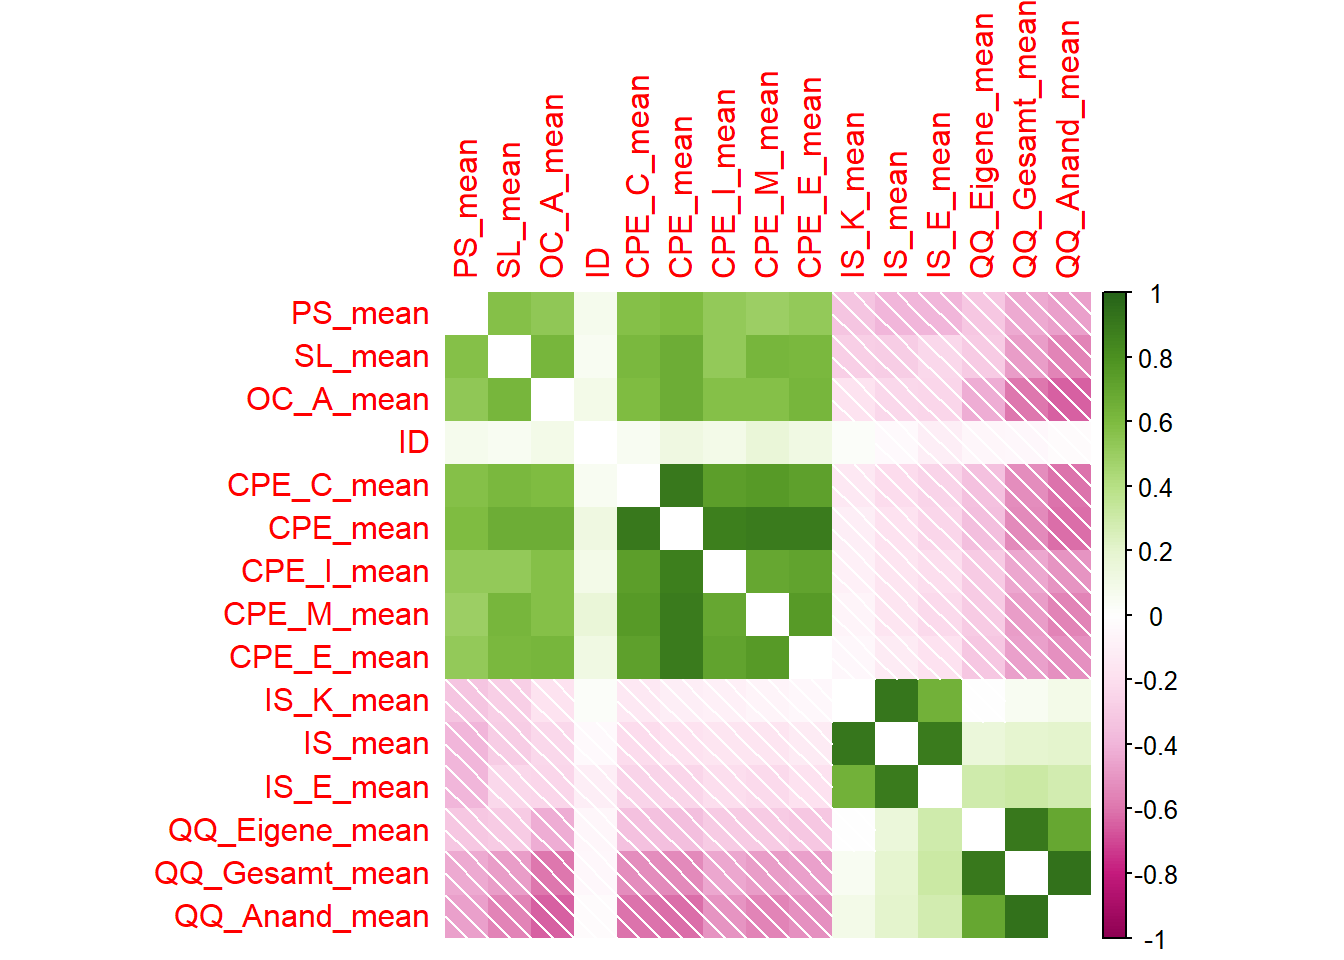
\includegraphics{0_Auswertung_files/figure-latex/unnamed-chunk-89-1.pdf}

\section{13. Überprüfung der
Hypothesen}\label{uxfcberpruxfcfung-der-hypothesen}

\subsection{Alter in Kategorien
unterteilen}\label{alter-in-kategorien-unterteilen}

\begin{Shaded}
\begin{Highlighting}[]
\NormalTok{d\_work\_lm }\OtherTok{\textless{}{-}}\NormalTok{ d\_work\_s }\SpecialCharTok{\%\textgreater{}\%} 
  \FunctionTok{mutate}\NormalTok{(}\AttributeTok{Alter\_kat =} \FunctionTok{case\_when}\NormalTok{(}
\NormalTok{    Alter }\SpecialCharTok{\textless{}=} \DecValTok{36} \SpecialCharTok{\textasciitilde{}} \StringTok{"jung"}\NormalTok{,}
\NormalTok{    Alter }\SpecialCharTok{\textgreater{}} \DecValTok{36} \SpecialCharTok{\textasciitilde{}} \StringTok{"alt"}
\NormalTok{  ))}
\end{Highlighting}
\end{Shaded}

\subsubsection{Mögliche Kontrollvariablen
testen}\label{muxf6gliche-kontrollvariablen-testen}

\begin{Shaded}
\begin{Highlighting}[]
\NormalTok{t\_test\_result\_QQ\_Alter }\OtherTok{\textless{}{-}} \FunctionTok{t.test}\NormalTok{(QQ\_Anand\_mean }\SpecialCharTok{\textasciitilde{}}\NormalTok{ Alter\_kat, }\AttributeTok{data =}\NormalTok{ d\_work\_lm)}
\FunctionTok{print}\NormalTok{(t\_test\_result\_QQ\_Alter)}
\end{Highlighting}
\end{Shaded}

\begin{verbatim}
## 
##  Welch Two Sample t-test
## 
## data:  QQ_Anand_mean by Alter_kat
## t = -2.7823, df = 150.97, p-value = 0.006087
## alternative hypothesis: true difference in means between group alt and group jung is not equal to 0
## 95 percent confidence interval:
##  -0.51798579 -0.08779796
## sample estimates:
##  mean in group alt mean in group jung 
##           2.101329           2.404221
\end{verbatim}

\begin{Shaded}
\begin{Highlighting}[]
\NormalTok{t\_test\_result\_CPE\_Alter }\OtherTok{\textless{}{-}} \FunctionTok{t.test}\NormalTok{(CPE\_mean }\SpecialCharTok{\textasciitilde{}}\NormalTok{ Alter\_kat, }\AttributeTok{data =}\NormalTok{ d\_work\_lm)}
\FunctionTok{print}\NormalTok{(t\_test\_result\_CPE\_Alter)}
\end{Highlighting}
\end{Shaded}

\begin{verbatim}
## 
##  Welch Two Sample t-test
## 
## data:  CPE_mean by Alter_kat
## t = 0.5386, df = 164, p-value = 0.5909
## alternative hypothesis: true difference in means between group alt and group jung is not equal to 0
## 95 percent confidence interval:
##  -0.2469154  0.4321471
## sample estimates:
##  mean in group alt mean in group jung 
##           4.898014           4.805398
\end{verbatim}

\begin{Shaded}
\begin{Highlighting}[]
\NormalTok{t\_test\_result\_PS\_Alter }\OtherTok{\textless{}{-}} \FunctionTok{t.test}\NormalTok{(PS\_mean }\SpecialCharTok{\textasciitilde{}}\NormalTok{ Alter\_kat, }\AttributeTok{data =}\NormalTok{ d\_work\_lm)}
\FunctionTok{print}\NormalTok{(t\_test\_result\_PS\_Alter)}
\end{Highlighting}
\end{Shaded}

\begin{verbatim}
## 
##  Welch Two Sample t-test
## 
## data:  PS_mean by Alter_kat
## t = 0.030328, df = 166.12, p-value = 0.9758
## alternative hypothesis: true difference in means between group alt and group jung is not equal to 0
## 95 percent confidence interval:
##  -0.3533158  0.3643396
## sample estimates:
##  mean in group alt mean in group jung 
##           5.456811           5.451299
\end{verbatim}

\begin{Shaded}
\begin{Highlighting}[]
\NormalTok{t\_test\_result\_IS\_Alter }\OtherTok{\textless{}{-}} \FunctionTok{t.test}\NormalTok{(IS\_mean }\SpecialCharTok{\textasciitilde{}}\NormalTok{ Alter\_kat, }\AttributeTok{data =}\NormalTok{ d\_work\_lm)}
\FunctionTok{print}\NormalTok{(t\_test\_result\_IS\_Alter)}
\end{Highlighting}
\end{Shaded}

\begin{verbatim}
## 
##  Welch Two Sample t-test
## 
## data:  IS_mean by Alter_kat
## t = -1.2916, df = 171.27, p-value = 0.1982
## alternative hypothesis: true difference in means between group alt and group jung is not equal to 0
## 95 percent confidence interval:
##  -0.6036727  0.1261357
## sample estimates:
##  mean in group alt mean in group jung 
##           3.056686           3.295455
\end{verbatim}

\begin{Shaded}
\begin{Highlighting}[]
\NormalTok{t\_test\_result\_SL\_Alter }\OtherTok{\textless{}{-}} \FunctionTok{t.test}\NormalTok{(SL\_mean }\SpecialCharTok{\textasciitilde{}}\NormalTok{ Alter\_kat, }\AttributeTok{data =}\NormalTok{ d\_work\_lm)}
\FunctionTok{print}\NormalTok{(t\_test\_result\_SL\_Alter)}
\end{Highlighting}
\end{Shaded}

\begin{verbatim}
## 
##  Welch Two Sample t-test
## 
## data:  SL_mean by Alter_kat
## t = 0.37259, df = 170.84, p-value = 0.7099
## alternative hypothesis: true difference in means between group alt and group jung is not equal to 0
## 95 percent confidence interval:
##  -0.3078619  0.4511218
## sample estimates:
##  mean in group alt mean in group jung 
##           4.532669           4.461039
\end{verbatim}

\begin{Shaded}
\begin{Highlighting}[]
\NormalTok{t\_test\_result\_OCA\_Alter }\OtherTok{\textless{}{-}} \FunctionTok{t.test}\NormalTok{(OC\_A\_mean }\SpecialCharTok{\textasciitilde{}}\NormalTok{ Alter\_kat, }\AttributeTok{data =}\NormalTok{ d\_work\_lm)}
\FunctionTok{print}\NormalTok{(t\_test\_result\_OCA\_Alter)}
\end{Highlighting}
\end{Shaded}

\begin{verbatim}
## 
##  Welch Two Sample t-test
## 
## data:  OC_A_mean by Alter_kat
## t = 1.9703, df = 163.37, p-value = 0.0505
## alternative hypothesis: true difference in means between group alt and group jung is not equal to 0
## 95 percent confidence interval:
##  -0.0006250448  0.5692296960
## sample estimates:
##  mean in group alt mean in group jung 
##           3.709302           3.425000
\end{verbatim}

\begin{Shaded}
\begin{Highlighting}[]
\NormalTok{lm\_PiU }\OtherTok{\textless{}{-}} \FunctionTok{lm}\NormalTok{(QQ\_Anand\_mean }\SpecialCharTok{\textasciitilde{}}\NormalTok{ Position\_im\_Unternehmen, }\AttributeTok{data=}\NormalTok{d\_work\_lm)}
\FunctionTok{plot}\NormalTok{(lm\_PiU)}
\end{Highlighting}
\end{Shaded}

\includegraphics{0_Auswertung_files/figure-latex/unnamed-chunk-97-1.pdf}
\includegraphics{0_Auswertung_files/figure-latex/unnamed-chunk-97-2.pdf}
\includegraphics{0_Auswertung_files/figure-latex/unnamed-chunk-97-3.pdf}
\includegraphics{0_Auswertung_files/figure-latex/unnamed-chunk-97-4.pdf}

\begin{Shaded}
\begin{Highlighting}[]
\NormalTok{lm\_BZG }\OtherTok{\textless{}{-}} \FunctionTok{lm}\NormalTok{(QQ\_Anand\_mean }\SpecialCharTok{\textasciitilde{}}\NormalTok{ BZG, }\AttributeTok{data=}\NormalTok{d\_work\_lm)}
\FunctionTok{plot}\NormalTok{(lm\_BZG)}
\end{Highlighting}
\end{Shaded}

\includegraphics{0_Auswertung_files/figure-latex/unnamed-chunk-98-1.pdf}
\includegraphics{0_Auswertung_files/figure-latex/unnamed-chunk-98-2.pdf}
\includegraphics{0_Auswertung_files/figure-latex/unnamed-chunk-98-3.pdf}
\includegraphics{0_Auswertung_files/figure-latex/unnamed-chunk-98-4.pdf}

\begin{quote}
Aufgrund der nicht signifikaten T-Tests mit der AV und den UVs ist
Alter\_kat nicht als Kontrollvariable geeignet. Da Gehalt\_n
möglicherweise eine Scheinkorrelation erzeugen würde, wird auch diese
nicht als Kontrollvariable in die Modell mit aufgenommen. Da die
Residuen der Variable BZG nicht normalverteilt ist und die Position im
Unternehmen
\end{quote}

\subsection{\texorpdfstring{H1: Kultur für psychologisches Empowerment -
\texttt{CPE}}{H1: Kultur für psychologisches Empowerment - CPE}}\label{h1-kultur-fuxfcr-psychologisches-empowerment---cpe}

\begin{Shaded}
\begin{Highlighting}[]
\NormalTok{lm1 }\OtherTok{\textless{}{-}} \FunctionTok{lm}\NormalTok{(QQ\_Anand\_mean }\SpecialCharTok{\textasciitilde{}}\NormalTok{ CPE\_mean, }\AttributeTok{data=}\NormalTok{d\_work\_lm)}
\FunctionTok{summary}\NormalTok{(lm1)}
\end{Highlighting}
\end{Shaded}

\begin{verbatim}
## 
## Call:
## lm(formula = QQ_Anand_mean ~ CPE_mean, data = d_work_lm)
## 
## Residuals:
##      Min       1Q   Median       3Q      Max 
## -1.56329 -0.37779 -0.01975  0.27640  1.78203 
## 
## Coefficients:
##             Estimate Std. Error t value Pr(>|t|)    
## (Intercept)  4.17691    0.19227   21.72   <2e-16 ***
## CPE_mean    -0.39643    0.03867  -10.25   <2e-16 ***
## ---
## Signif. codes:  0 '***' 0.001 '**' 0.01 '*' 0.05 '.' 0.1 ' ' 1
## 
## Residual standard error: 0.5791 on 174 degrees of freedom
## Multiple R-squared:  0.3766, Adjusted R-squared:  0.373 
## F-statistic: 105.1 on 1 and 174 DF,  p-value: < 2.2e-16
\end{verbatim}

\begin{quote}
signifikater Zusammenahng mit einer erklärten Varianz von ca. 38 \%
\end{quote}

\begin{Shaded}
\begin{Highlighting}[]
\FunctionTok{confint}\NormalTok{(lm1)}
\end{Highlighting}
\end{Shaded}

\begin{verbatim}
##                  2.5 %     97.5 %
## (Intercept)  3.7974202  4.5563920
## CPE_mean    -0.4727547 -0.3201066
\end{verbatim}

\subsubsection{Effektgröße
beschreiben}\label{effektgruxf6uxdfe-beschreiben}

\begin{Shaded}
\begin{Highlighting}[]
\NormalTok{effectsize}\SpecialCharTok{::}\FunctionTok{interpret\_r2}\NormalTok{(}\FloatTok{0.3766}\NormalTok{, }\AttributeTok{rules=}\StringTok{"cohen1988"}\NormalTok{)}
\end{Highlighting}
\end{Shaded}

\begin{verbatim}
## [1] "substantial"
## (Rules: cohen1988)
\end{verbatim}

\subsection{\texorpdfstring{H2: Organisationales Commitment - affektiv
\texttt{OCA}}{H2: Organisationales Commitment - affektiv OCA}}\label{h2-organisationales-commitment---affektiv-oca}

\begin{Shaded}
\begin{Highlighting}[]
\NormalTok{lm2 }\OtherTok{\textless{}{-}} \FunctionTok{lm}\NormalTok{(QQ\_Anand\_mean }\SpecialCharTok{\textasciitilde{}}\NormalTok{ OC\_A\_mean, }\AttributeTok{data=}\NormalTok{d\_work\_lm)}
\FunctionTok{summary}\NormalTok{(lm2)}
\end{Highlighting}
\end{Shaded}

\begin{verbatim}
## 
## Call:
## lm(formula = QQ_Anand_mean ~ OC_A_mean, data = d_work_lm)
## 
## Residuals:
##      Min       1Q   Median       3Q      Max 
## -1.40215 -0.33546 -0.04383  0.30010  1.96012 
## 
## Coefficients:
##             Estimate Std. Error t value Pr(>|t|)    
## (Intercept)  3.99726    0.16132   24.78   <2e-16 ***
## OC_A_mean   -0.48935    0.04379  -11.17   <2e-16 ***
## ---
## Signif. codes:  0 '***' 0.001 '**' 0.01 '*' 0.05 '.' 0.1 ' ' 1
## 
## Residual standard error: 0.5596 on 174 degrees of freedom
## Multiple R-squared:  0.4178, Adjusted R-squared:  0.4144 
## F-statistic: 124.9 on 1 and 174 DF,  p-value: < 2.2e-16
\end{verbatim}

\begin{quote}
signifikater Zusammenahng mit einer erklärten Varianz von ca. 42 \%
\end{quote}

\subsubsection{Effektgröße
beschreiben}\label{effektgruxf6uxdfe-beschreiben-1}

\begin{Shaded}
\begin{Highlighting}[]
\NormalTok{effectsize}\SpecialCharTok{::}\FunctionTok{interpret\_r2}\NormalTok{(}\FloatTok{0.4178}\NormalTok{, }\AttributeTok{rules=}\StringTok{"cohen1988"}\NormalTok{)}
\end{Highlighting}
\end{Shaded}

\begin{verbatim}
## [1] "substantial"
## (Rules: cohen1988)
\end{verbatim}

\begin{Shaded}
\begin{Highlighting}[]
\FunctionTok{confint}\NormalTok{(lm2)}
\end{Highlighting}
\end{Shaded}

\begin{verbatim}
##                  2.5 %     97.5 %
## (Intercept)  3.6788563  4.3156663
## OC_A_mean   -0.5757782 -0.4029124
\end{verbatim}

\subsection{\texorpdfstring{H3: Psychologische Sicherheit
\texttt{PS}}{H3: Psychologische Sicherheit PS}}\label{h3-psychologische-sicherheit-ps}

\begin{Shaded}
\begin{Highlighting}[]
\NormalTok{lm3 }\OtherTok{\textless{}{-}} \FunctionTok{lm}\NormalTok{(QQ\_Anand\_mean }\SpecialCharTok{\textasciitilde{}}\NormalTok{ PS\_mean, }\AttributeTok{data=}\NormalTok{d\_work\_lm)}
\FunctionTok{summary}\NormalTok{(lm3)}
\end{Highlighting}
\end{Shaded}

\begin{verbatim}
## 
## Call:
## lm(formula = QQ_Anand_mean ~ PS_mean, data = d_work_lm)
## 
## Residuals:
##      Min       1Q   Median       3Q      Max 
## -1.11980 -0.43197 -0.05837  0.33547  2.45261 
## 
## Coefficients:
##             Estimate Std. Error t value Pr(>|t|)    
## (Intercept)  3.81901    0.22884  16.688  < 2e-16 ***
## PS_mean     -0.28670    0.04104  -6.985 5.78e-11 ***
## ---
## Signif. codes:  0 '***' 0.001 '**' 0.01 '*' 0.05 '.' 0.1 ' ' 1
## 
## Residual standard error: 0.6481 on 174 degrees of freedom
## Multiple R-squared:  0.219,  Adjusted R-squared:  0.2145 
## F-statistic:  48.8 on 1 and 174 DF,  p-value: 5.784e-11
\end{verbatim}

\begin{quote}
signifikater Zusammenahng mit einer erklärten Varianz von ca. 22 \%
\end{quote}

\subsubsection{Effektgröße
beschreiben}\label{effektgruxf6uxdfe-beschreiben-2}

\begin{Shaded}
\begin{Highlighting}[]
\NormalTok{effectsize}\SpecialCharTok{::}\FunctionTok{interpret\_r2}\NormalTok{(}\FloatTok{0.219}\NormalTok{, }\AttributeTok{rules=}\StringTok{"cohen1988"}\NormalTok{)}
\end{Highlighting}
\end{Shaded}

\begin{verbatim}
## [1] "moderate"
## (Rules: cohen1988)
\end{verbatim}

\begin{Shaded}
\begin{Highlighting}[]
\FunctionTok{confint}\NormalTok{(lm3)}
\end{Highlighting}
\end{Shaded}

\begin{verbatim}
##                  2.5 %     97.5 %
## (Intercept)  3.3673447  4.2706720
## PS_mean     -0.3677007 -0.2056918
\end{verbatim}

\subsection{\texorpdfstring{H4: Irritation
\texttt{IS}}{H4: Irritation IS}}\label{h4-irritation-is}

\begin{Shaded}
\begin{Highlighting}[]
\NormalTok{lm4 }\OtherTok{\textless{}{-}} \FunctionTok{lm}\NormalTok{(QQ\_Anand\_mean }\SpecialCharTok{\textasciitilde{}}\NormalTok{ IS\_mean, }\AttributeTok{data=}\NormalTok{d\_work\_lm)}
\FunctionTok{summary}\NormalTok{(lm4)}
\end{Highlighting}
\end{Shaded}

\begin{verbatim}
## 
## Call:
## lm(formula = QQ_Anand_mean ~ IS_mean, data = d_work_lm)
## 
## Residuals:
##      Min       1Q   Median       3Q      Max 
## -1.35612 -0.47978 -0.09595  0.38609  2.25600 
## 
## Coefficients:
##             Estimate Std. Error t value Pr(>|t|)    
## (Intercept)  1.86665    0.15102  12.361   <2e-16 ***
## IS_mean      0.12237    0.04416   2.771   0.0062 ** 
## ---
## Signif. codes:  0 '***' 0.001 '**' 0.01 '*' 0.05 '.' 0.1 ' ' 1
## 
## Residual standard error: 0.7177 on 174 degrees of freedom
## Multiple R-squared:  0.04226,    Adjusted R-squared:  0.03675 
## F-statistic: 7.677 on 1 and 174 DF,  p-value: 0.006201
\end{verbatim}

\begin{quote}
signifikater Zusammenahng mit einer erklärten Varianz von ca. 4 \%
\end{quote}

\subsubsection{Effektgröße
beschreiben}\label{effektgruxf6uxdfe-beschreiben-3}

\begin{Shaded}
\begin{Highlighting}[]
\NormalTok{effectsize}\SpecialCharTok{::}\FunctionTok{interpret\_r2}\NormalTok{(}\FloatTok{0.04226}\NormalTok{, }\AttributeTok{rules=}\StringTok{"cohen1988"}\NormalTok{)}
\end{Highlighting}
\end{Shaded}

\begin{verbatim}
## [1] "weak"
## (Rules: cohen1988)
\end{verbatim}

\begin{Shaded}
\begin{Highlighting}[]
\FunctionTok{confint}\NormalTok{(lm4)}
\end{Highlighting}
\end{Shaded}

\begin{verbatim}
##                  2.5 %    97.5 %
## (Intercept) 1.56859369 2.1647140
## IS_mean     0.03520003 0.2095328
\end{verbatim}

\subsection{\texorpdfstring{H5: Servant Leadership
\texttt{SL}}{H5: Servant Leadership SL}}\label{h5-servant-leadership-sl}

\begin{Shaded}
\begin{Highlighting}[]
\NormalTok{lm5 }\OtherTok{\textless{}{-}} \FunctionTok{lm}\NormalTok{(QQ\_Anand\_mean }\SpecialCharTok{\textasciitilde{}}\NormalTok{ SL\_mean, }\AttributeTok{data=}\NormalTok{d\_work\_lm)}
\FunctionTok{summary}\NormalTok{(lm5)}
\end{Highlighting}
\end{Shaded}

\begin{verbatim}
## 
## Call:
## lm(formula = QQ_Anand_mean ~ SL_mean, data = d_work_lm)
## 
## Residuals:
##      Min       1Q   Median       3Q      Max 
## -1.31955 -0.42335 -0.06577  0.32378  1.95465 
## 
## Coefficients:
##             Estimate Std. Error t value Pr(>|t|)    
## (Intercept)  3.67448    0.16827  21.837  < 2e-16 ***
## SL_mean     -0.31678    0.03618  -8.756 1.73e-15 ***
## ---
## Signif. codes:  0 '***' 0.001 '**' 0.01 '*' 0.05 '.' 0.1 ' ' 1
## 
## Residual standard error: 0.611 on 174 degrees of freedom
## Multiple R-squared:  0.3059, Adjusted R-squared:  0.3019 
## F-statistic: 76.68 on 1 and 174 DF,  p-value: 1.729e-15
\end{verbatim}

\begin{quote}
signifikater Zusammenahng mit einer erklärten Varianz von ca. 31 \%
\end{quote}

\begin{Shaded}
\begin{Highlighting}[]
\FunctionTok{confint}\NormalTok{(lm5)}
\end{Highlighting}
\end{Shaded}

\begin{verbatim}
##                  2.5 %     97.5 %
## (Intercept)  3.3423713  4.0065941
## SL_mean     -0.3881762 -0.2453754
\end{verbatim}

\subsubsection{Effektgröße
beschreiben}\label{effektgruxf6uxdfe-beschreiben-4}

\begin{Shaded}
\begin{Highlighting}[]
\NormalTok{effectsize}\SpecialCharTok{::}\FunctionTok{interpret\_r2}\NormalTok{(}\FloatTok{0.3059}\NormalTok{, }\AttributeTok{rules=}\StringTok{"cohen1988"}\NormalTok{)}
\end{Highlighting}
\end{Shaded}

\begin{verbatim}
## [1] "substantial"
## (Rules: cohen1988)
\end{verbatim}

\section{H2.2: Moderation: CPE moderiert den Zusammenhang von OCA und
QQ}\label{h2.2-moderation-cpe-moderiert-den-zusammenhang-von-oca-und-qq}

\begin{Shaded}
\begin{Highlighting}[]
\NormalTok{d\_work\_plot\_lm }\OtherTok{\textless{}{-}}\NormalTok{ d\_work\_s }\SpecialCharTok{\%\textgreater{}\%} 
  \FunctionTok{mutate}\NormalTok{(}\AttributeTok{CPE =} \FunctionTok{case\_when}\NormalTok{(}
\NormalTok{    CPE\_mean }\SpecialCharTok{\textless{}=} \FloatTok{3.99} \SpecialCharTok{\textasciitilde{}} \StringTok{"CPE\_no"}\NormalTok{,}
\NormalTok{    CPE\_mean }\SpecialCharTok{\textgreater{}} \FloatTok{3.99} \SpecialCharTok{\&}\NormalTok{ CPE\_mean }\SpecialCharTok{\textless{}} \FloatTok{4.99} \SpecialCharTok{\textasciitilde{}} \StringTok{"CPE\_neutral"}\NormalTok{,}
\NormalTok{    CPE\_mean }\SpecialCharTok{\textgreater{}=} \FloatTok{4.99} \SpecialCharTok{\textasciitilde{}} \StringTok{"CPE\_yes"}
\NormalTok{  ))}
\end{Highlighting}
\end{Shaded}

\subsection{Visuelle Darstellung des möglichen
Zusammenhangs}\label{visuelle-darstellung-des-muxf6glichen-zusammenhangs}

\begin{Shaded}
\begin{Highlighting}[]
\FunctionTok{ggplot}\NormalTok{(d\_work\_plot\_lm)}\SpecialCharTok{+}
  \FunctionTok{geom\_jitter}\NormalTok{(}\AttributeTok{mapping =} \FunctionTok{aes}\NormalTok{(}\AttributeTok{x=}\NormalTok{OC\_A\_mean, }\AttributeTok{y=}\NormalTok{QQ\_Anand\_mean))}\SpecialCharTok{+}
  \FunctionTok{geom\_smooth}\NormalTok{(}\AttributeTok{mapping =} \FunctionTok{aes}\NormalTok{(}\AttributeTok{x=}\NormalTok{OC\_A\_mean, }\AttributeTok{y=}\NormalTok{QQ\_Anand\_mean, }\AttributeTok{color=}\FunctionTok{as.factor}\NormalTok{(CPE)), }\AttributeTok{method =} \StringTok{"lm"}\NormalTok{, }\AttributeTok{se=}\ConstantTok{FALSE}\NormalTok{)}\SpecialCharTok{+}
  \FunctionTok{theme\_minimal}\NormalTok{()}
\end{Highlighting}
\end{Shaded}

\begin{verbatim}
## `geom_smooth()` using formula = 'y ~ x'
\end{verbatim}

\includegraphics{0_Auswertung_files/figure-latex/unnamed-chunk-115-1.pdf}

\begin{Shaded}
\begin{Highlighting}[]
\NormalTok{lm6 }\OtherTok{\textless{}{-}} \FunctionTok{lm}\NormalTok{(QQ\_Anand\_mean }\SpecialCharTok{\textasciitilde{}}\NormalTok{ OC\_A\_mean}\SpecialCharTok{*}\NormalTok{CPE\_mean, }\AttributeTok{data=}\NormalTok{d\_work\_lm)}
\FunctionTok{summary}\NormalTok{(lm6)}
\end{Highlighting}
\end{Shaded}

\begin{verbatim}
## 
## Call:
## lm(formula = QQ_Anand_mean ~ OC_A_mean * CPE_mean, data = d_work_lm)
## 
## Residuals:
##      Min       1Q   Median       3Q      Max 
## -1.67371 -0.35216 -0.03223  0.32281  1.78792 
## 
## Coefficients:
##                    Estimate Std. Error t value Pr(>|t|)    
## (Intercept)         5.14769    0.51506   9.994  < 2e-16 ***
## OC_A_mean          -0.54964    0.16334  -3.365 0.000944 ***
## CPE_mean           -0.37709    0.12119  -3.112 0.002180 ** 
## OC_A_mean:CPE_mean  0.04960    0.03369   1.473 0.142708    
## ---
## Signif. codes:  0 '***' 0.001 '**' 0.01 '*' 0.05 '.' 0.1 ' ' 1
## 
## Residual standard error: 0.5295 on 172 degrees of freedom
## Multiple R-squared:  0.4848, Adjusted R-squared:  0.4758 
## F-statistic: 53.95 on 3 and 172 DF,  p-value: < 2.2e-16
\end{verbatim}

\begin{quote}
Keinen signifikante Moderation!
\end{quote}

\begin{Shaded}
\begin{Highlighting}[]
\FunctionTok{library}\NormalTok{(interactions)}
\end{Highlighting}
\end{Shaded}

\begin{verbatim}
## Warning: Paket 'interactions' wurde unter R Version 4.3.3 erstellt
\end{verbatim}

\begin{Shaded}
\begin{Highlighting}[]
\NormalTok{plot\_lm6 }\OtherTok{\textless{}{-}}\FunctionTok{interact\_plot}\NormalTok{(}\AttributeTok{model=}\NormalTok{lm6, }\AttributeTok{pred=}\NormalTok{OC\_A\_mean, }\AttributeTok{modx=}\NormalTok{CPE\_mean)}
\NormalTok{plot\_lm6}
\end{Highlighting}
\end{Shaded}

\includegraphics{0_Auswertung_files/figure-latex/unnamed-chunk-117-1.pdf}

\begin{Shaded}
\begin{Highlighting}[]
\FunctionTok{svg}\NormalTok{(}\StringTok{"H2.2.svg"}\NormalTok{, }\AttributeTok{width =} \DecValTok{7}\NormalTok{, }\AttributeTok{height =} \DecValTok{5}\NormalTok{)}
\FunctionTok{print}\NormalTok{(plot\_lm6)}
\FunctionTok{dev.off}\NormalTok{()}
\end{Highlighting}
\end{Shaded}

\begin{verbatim}
## pdf 
##   2
\end{verbatim}

\section{H2.1: Moderation: Alter moderiert den Zusammenhang von OCA und
QQ-Gesamt}\label{h2.1-moderation-alter-moderiert-den-zusammenhang-von-oca-und-qq-gesamt}

\begin{Shaded}
\begin{Highlighting}[]
\FunctionTok{ggplot}\NormalTok{(d\_work\_lm)}\SpecialCharTok{+}
  \FunctionTok{geom\_jitter}\NormalTok{(}\AttributeTok{mapping =} \FunctionTok{aes}\NormalTok{(}\AttributeTok{x=}\NormalTok{OC\_A\_mean, }\AttributeTok{y=}\NormalTok{QQ\_Gesamt\_mean, }\AttributeTok{color=}\FunctionTok{as.factor}\NormalTok{(Alter\_kat)))}\SpecialCharTok{+}
  \FunctionTok{geom\_smooth}\NormalTok{(}\AttributeTok{mapping =} \FunctionTok{aes}\NormalTok{(}\AttributeTok{x=}\NormalTok{OC\_A\_mean, }\AttributeTok{y=}\NormalTok{QQ\_Gesamt\_mean, }\AttributeTok{color=}\FunctionTok{as.factor}\NormalTok{(Alter\_kat)), }\AttributeTok{method =} \StringTok{"lm"}\NormalTok{, }\AttributeTok{se=}\ConstantTok{FALSE}\NormalTok{)}
\end{Highlighting}
\end{Shaded}

\begin{verbatim}
## `geom_smooth()` using formula = 'y ~ x'
\end{verbatim}

\includegraphics{0_Auswertung_files/figure-latex/unnamed-chunk-119-1.pdf}

\subsection{QQ\_Anand}\label{qq_anand}

\begin{Shaded}
\begin{Highlighting}[]
\NormalTok{lm7 }\OtherTok{\textless{}{-}} \FunctionTok{lm}\NormalTok{(QQ\_Anand\_mean }\SpecialCharTok{\textasciitilde{}}\NormalTok{ OC\_A\_mean}\SpecialCharTok{*}\NormalTok{Alter\_kat, }\AttributeTok{data=}\NormalTok{d\_work\_lm)}
\FunctionTok{summary}\NormalTok{(lm7)}
\end{Highlighting}
\end{Shaded}

\begin{verbatim}
## 
## Call:
## lm(formula = QQ_Anand_mean ~ OC_A_mean * Alter_kat, data = d_work_lm)
## 
## Residuals:
##      Min       1Q   Median       3Q      Max 
## -1.23827 -0.36525 -0.00935  0.28869  1.99065 
## 
## Coefficients:
##                         Estimate Std. Error t value Pr(>|t|)    
## (Intercept)              3.27496    0.27237  12.024  < 2e-16 ***
## OC_A_mean               -0.31640    0.07170  -4.413 1.81e-05 ***
## Alter_katjung            1.11431    0.33578   3.319  0.00111 ** 
## OC_A_mean:Alter_katjung -0.26318    0.09023  -2.917  0.00401 ** 
## ---
## Signif. codes:  0 '***' 0.001 '**' 0.01 '*' 0.05 '.' 0.1 ' ' 1
## 
## Residual standard error: 0.5448 on 170 degrees of freedom
##   (2 Beobachtungen als fehlend gelöscht)
## Multiple R-squared:  0.4601, Adjusted R-squared:  0.4506 
## F-statistic:  48.3 on 3 and 170 DF,  p-value: < 2.2e-16
\end{verbatim}

\begin{Shaded}
\begin{Highlighting}[]
\FunctionTok{confint}\NormalTok{(lm7)}
\end{Highlighting}
\end{Shaded}

\begin{verbatim}
##                              2.5 %     97.5 %
## (Intercept)              2.7373003  3.8126292
## OC_A_mean               -0.4579419 -0.1748649
## Alter_katjung            0.4514827  1.7771444
## OC_A_mean:Alter_katjung -0.4412825 -0.0850684
\end{verbatim}

\begin{Shaded}
\begin{Highlighting}[]
\NormalTok{plot\_lm7 }\OtherTok{\textless{}{-}}\FunctionTok{interact\_plot}\NormalTok{(}\AttributeTok{model=}\NormalTok{lm7, }\AttributeTok{pred=}\NormalTok{OC\_A\_mean, }\AttributeTok{modx=}\NormalTok{Alter\_kat,}
              \AttributeTok{interval =} \ConstantTok{TRUE}\NormalTok{)}
\NormalTok{plot\_lm7}
\end{Highlighting}
\end{Shaded}

\includegraphics{0_Auswertung_files/figure-latex/unnamed-chunk-122-1.pdf}

\begin{Shaded}
\begin{Highlighting}[]
\FunctionTok{svg}\NormalTok{(}\StringTok{"H2.1.svg"}\NormalTok{, }\AttributeTok{width =} \DecValTok{7}\NormalTok{, }\AttributeTok{height =} \DecValTok{5}\NormalTok{)}
\FunctionTok{print}\NormalTok{(plot\_lm7)}
\FunctionTok{dev.off}\NormalTok{()}
\end{Highlighting}
\end{Shaded}

\begin{verbatim}
## pdf 
##   2
\end{verbatim}

\end{document}
